% figures.tex — all figures for the Vitrine v5 report
% Include in the main document body with % figures.tex — all figures for the Vitrine v5 report
% Include in the main document body with % figures.tex — all figures for the Vitrine v5 report
% Include in the main document body with % figures.tex — all figures for the Vitrine v5 report
% Include in the main document body with \input{figures}
% Assumes \graphicspath{{figures/}} is set in the preamble (relative to report/v5/).
%
% Labels (for \ref / \autoref):
%   fig:router           — capture-adaptive router flowchart
%   fig:component_menu   — component-menu status flowchart
%   fig:architecture     — system architecture (container topology)
%   fig:nanogs_room      — NanoGS real-Gaussian splat render (canonical room hero)
%   fig:scene_integrated — fully integrated UE 5.8 scene (room + objects)
%   fig:objects          — TRELLIS.2 object turnaround sheet (chair)
%   fig:ue_come          — CoMe-TSDF mesh game asset in UE (baseline mesh)
%   fig:ue_nanogs        — NanoGS splat render (dreamlab room, 1920x1080)
%   fig:ue_hero          — Hero perspective render (room + placed objects)
%   fig:ue_dollhouse     — Overhead dollhouse view of integrated UE scene

% ──────────────────────────────────────────────────────────────────────────────
% 1. Capture-adaptive router
% ──────────────────────────────────────────────────────────────────────────────
\begin{figure}[htbp]
  \centering
  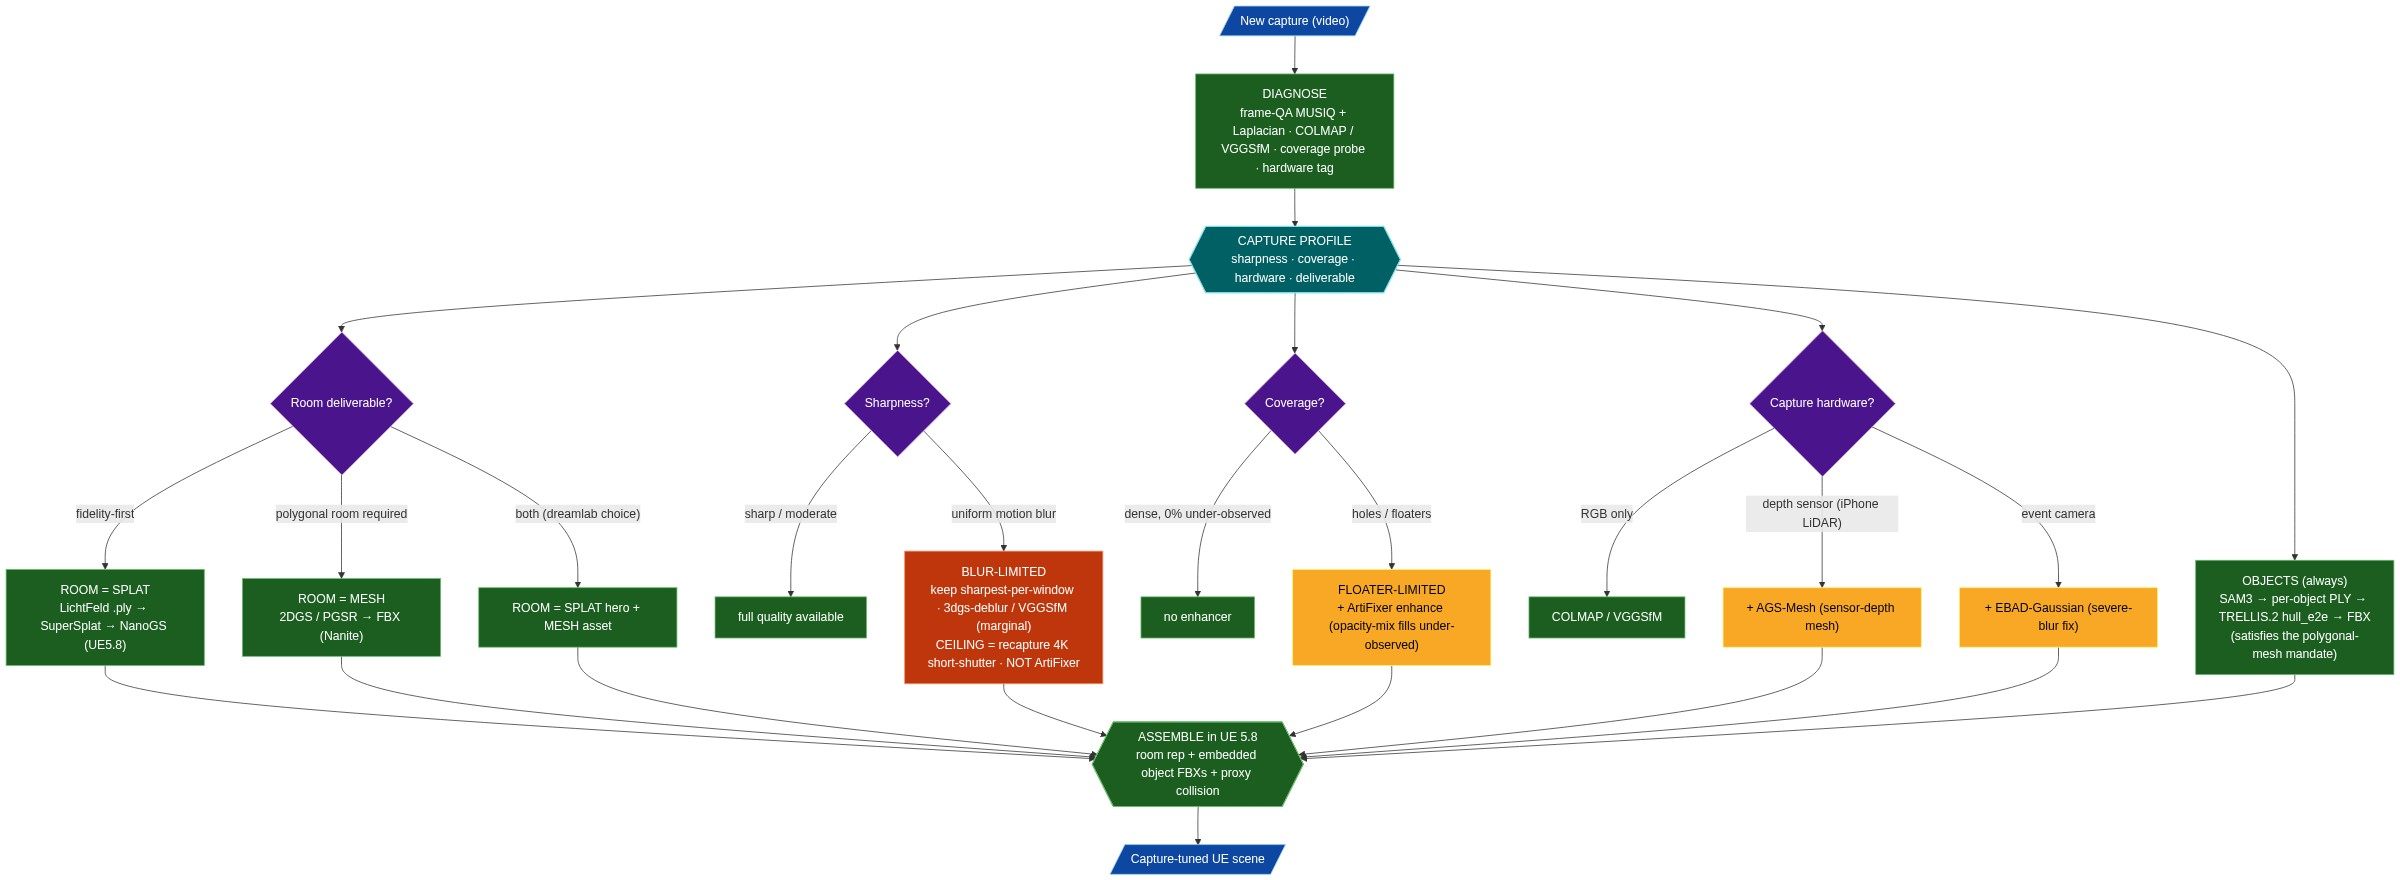
\includegraphics[width=\textwidth]{figures/router.jpg}
  \caption{%
    \textbf{Capture-adaptive router.}
    The pipeline diagnoses each new capture on four axes
    (sharpness via MUSIQ + full-resolution Laplacian, coverage via occupancy probe,
    available hardware, and deliverable type) and selects the configuration that
    fits the bottleneck.
    Green nodes are validated keepers; orange nodes are
    capture-conditional options; red nodes are blur-limited warnings.
    The dreamlab capture routes to Opt\,4 (splat hero + mesh asset + TRELLIS.2 objects)
    with a recapture flag as the quality ceiling.
  }
  \label{fig:router}
\end{figure}

% ──────────────────────────────────────────────────────────────────────────────
% 2. Component-menu flowchart
% ──────────────────────────────────────────────────────────────────────────────
\begin{figure}[htbp]
  \centering
  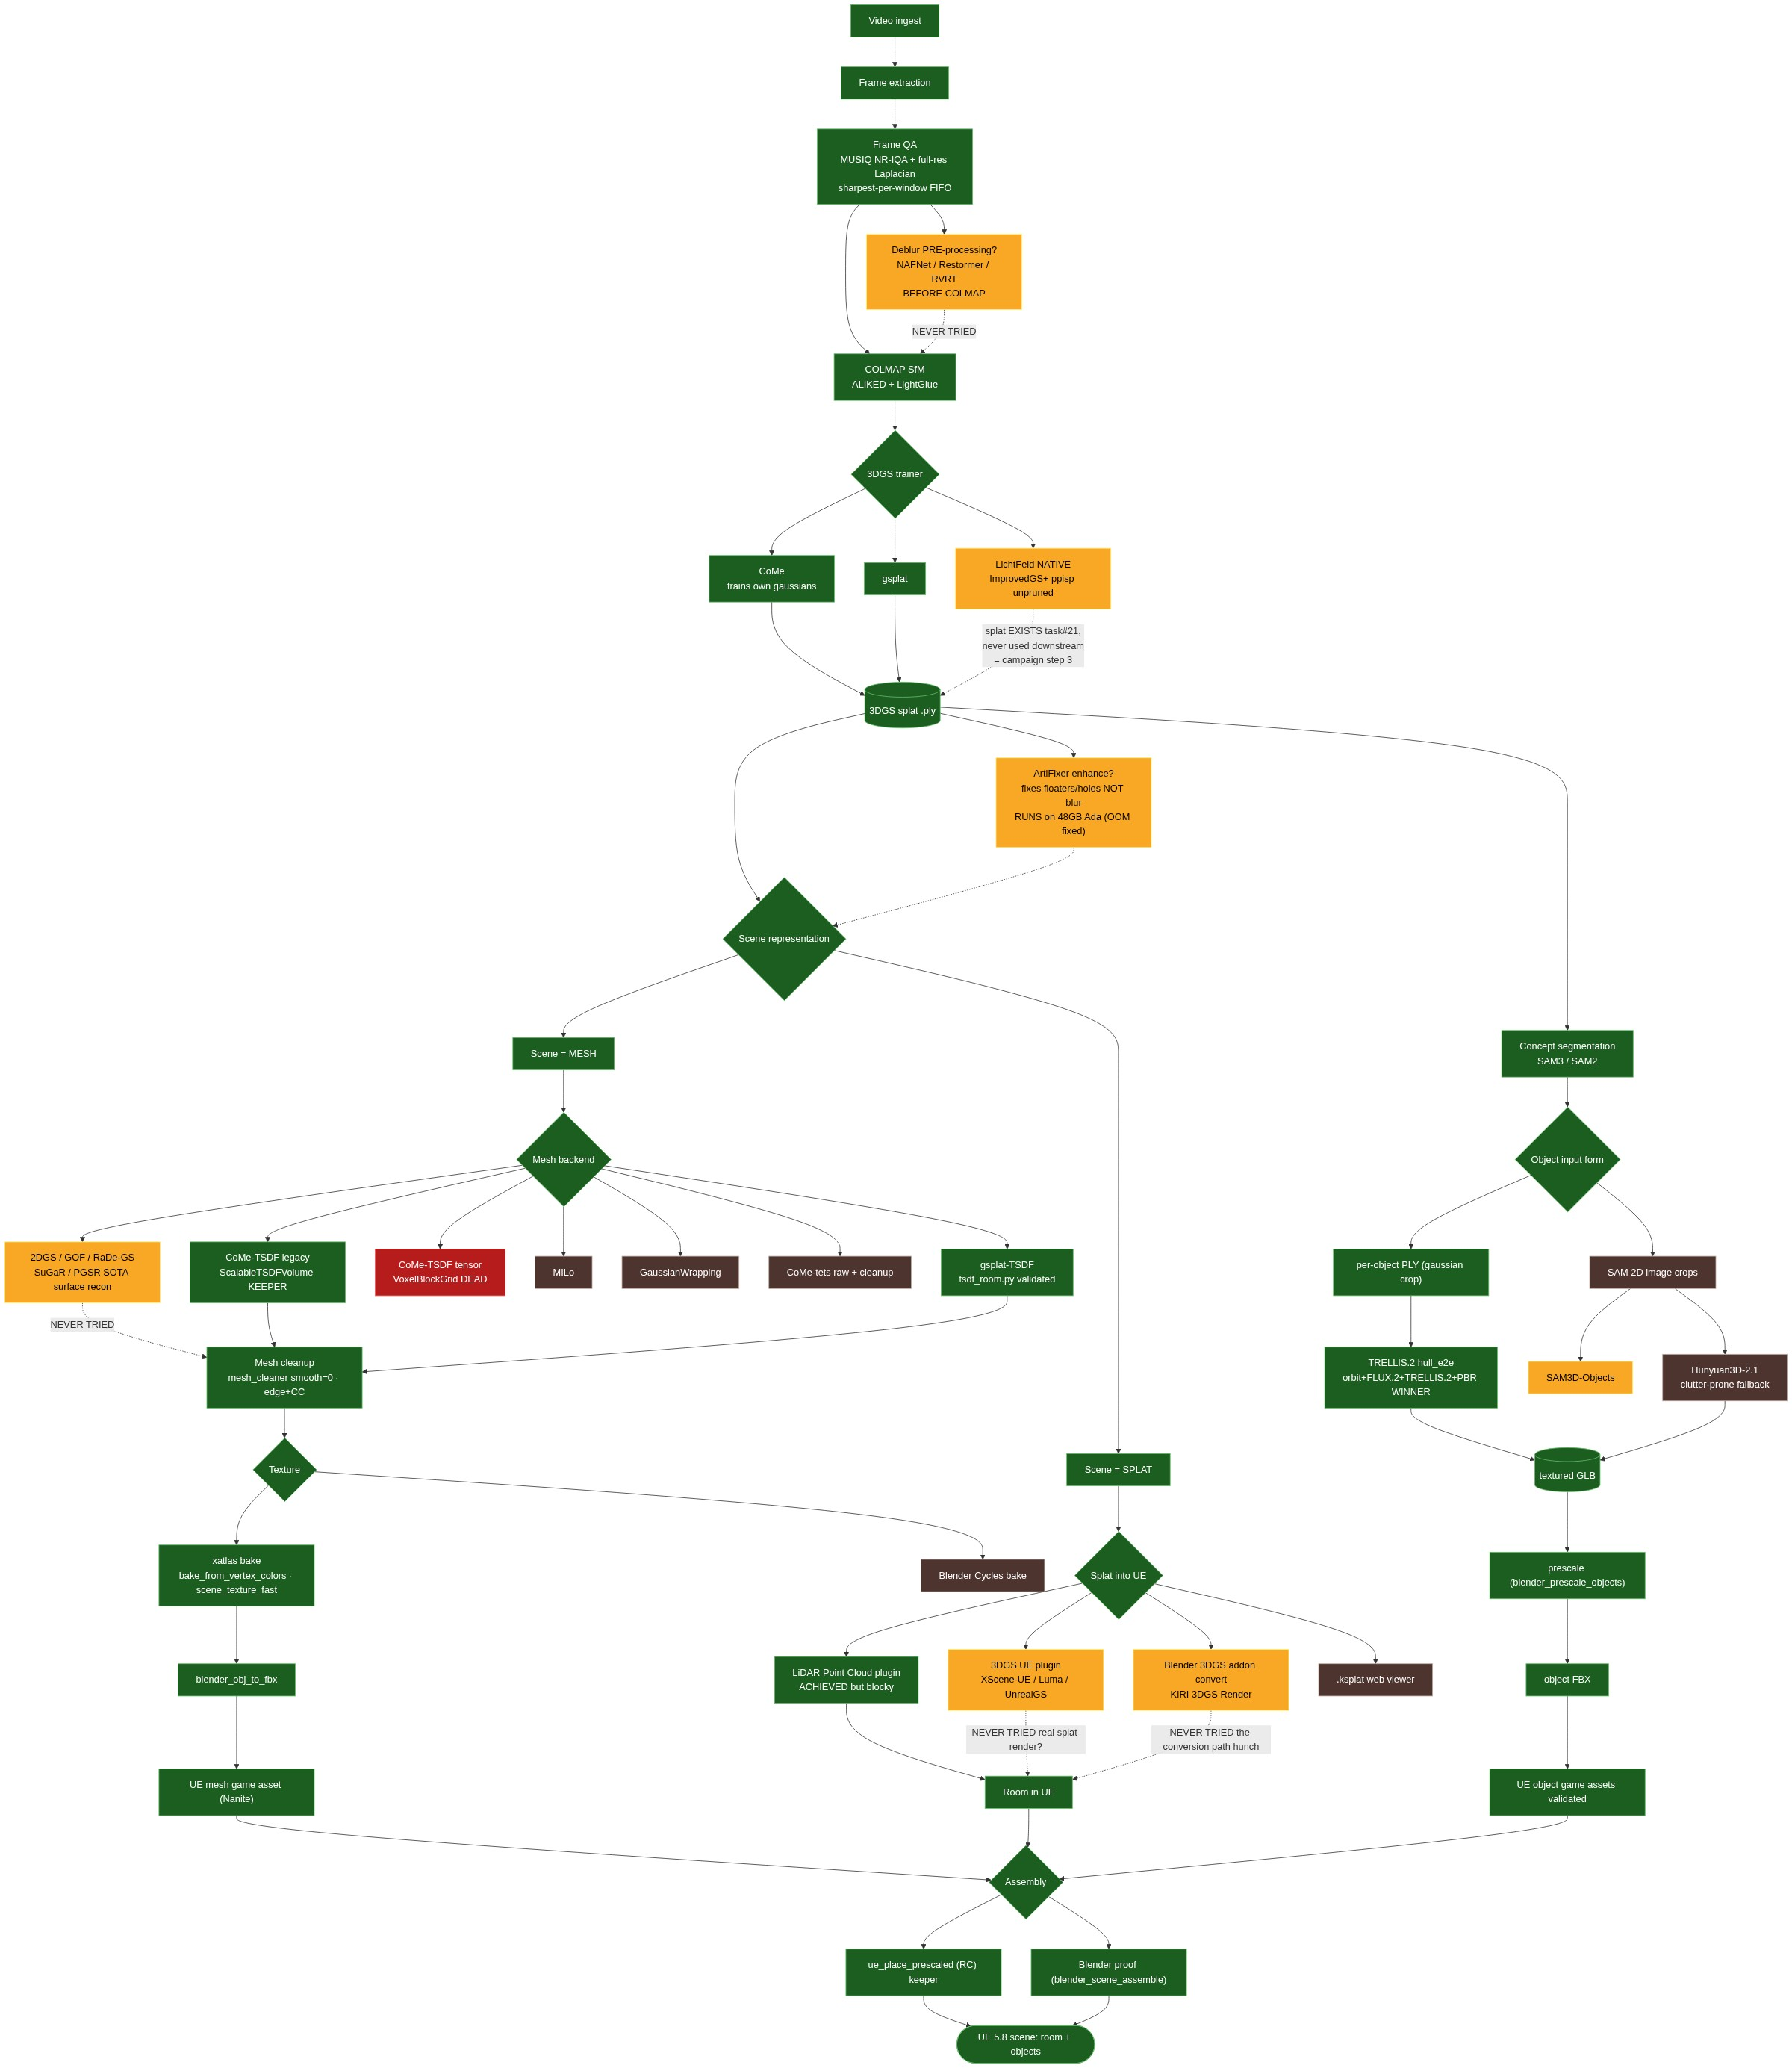
\includegraphics[width=\textwidth]{figures/component_menu.jpg}
  \caption{%
    \textbf{Full component-menu status chart (validated 2026-06-25).}
    Every branch of the Vitrine toolkit from video ingest to UE\,5.8 delivery.
    Colour coding: \emph{green} = validated keeper in active use;
    \emph{brown} = exercised but subordinate / fallback;
    \emph{red} = tried and abandoned;
    \emph{yellow} = plausible, never run.
    The chart is the canonical record of what has and has not been exercised;
    dashed arrows mark paths that remain open research items
    (SAM3D-Objects, BAD-Gaussians deblur, PGSR/2DGS surface reconstruction).
  }
  \label{fig:component_menu}
\end{figure}

% ──────────────────────────────────────────────────────────────────────────────
% 3. System architecture (container topology)
% ──────────────────────────────────────────────────────────────────────────────
\begin{figure}[htbp]
  \centering
  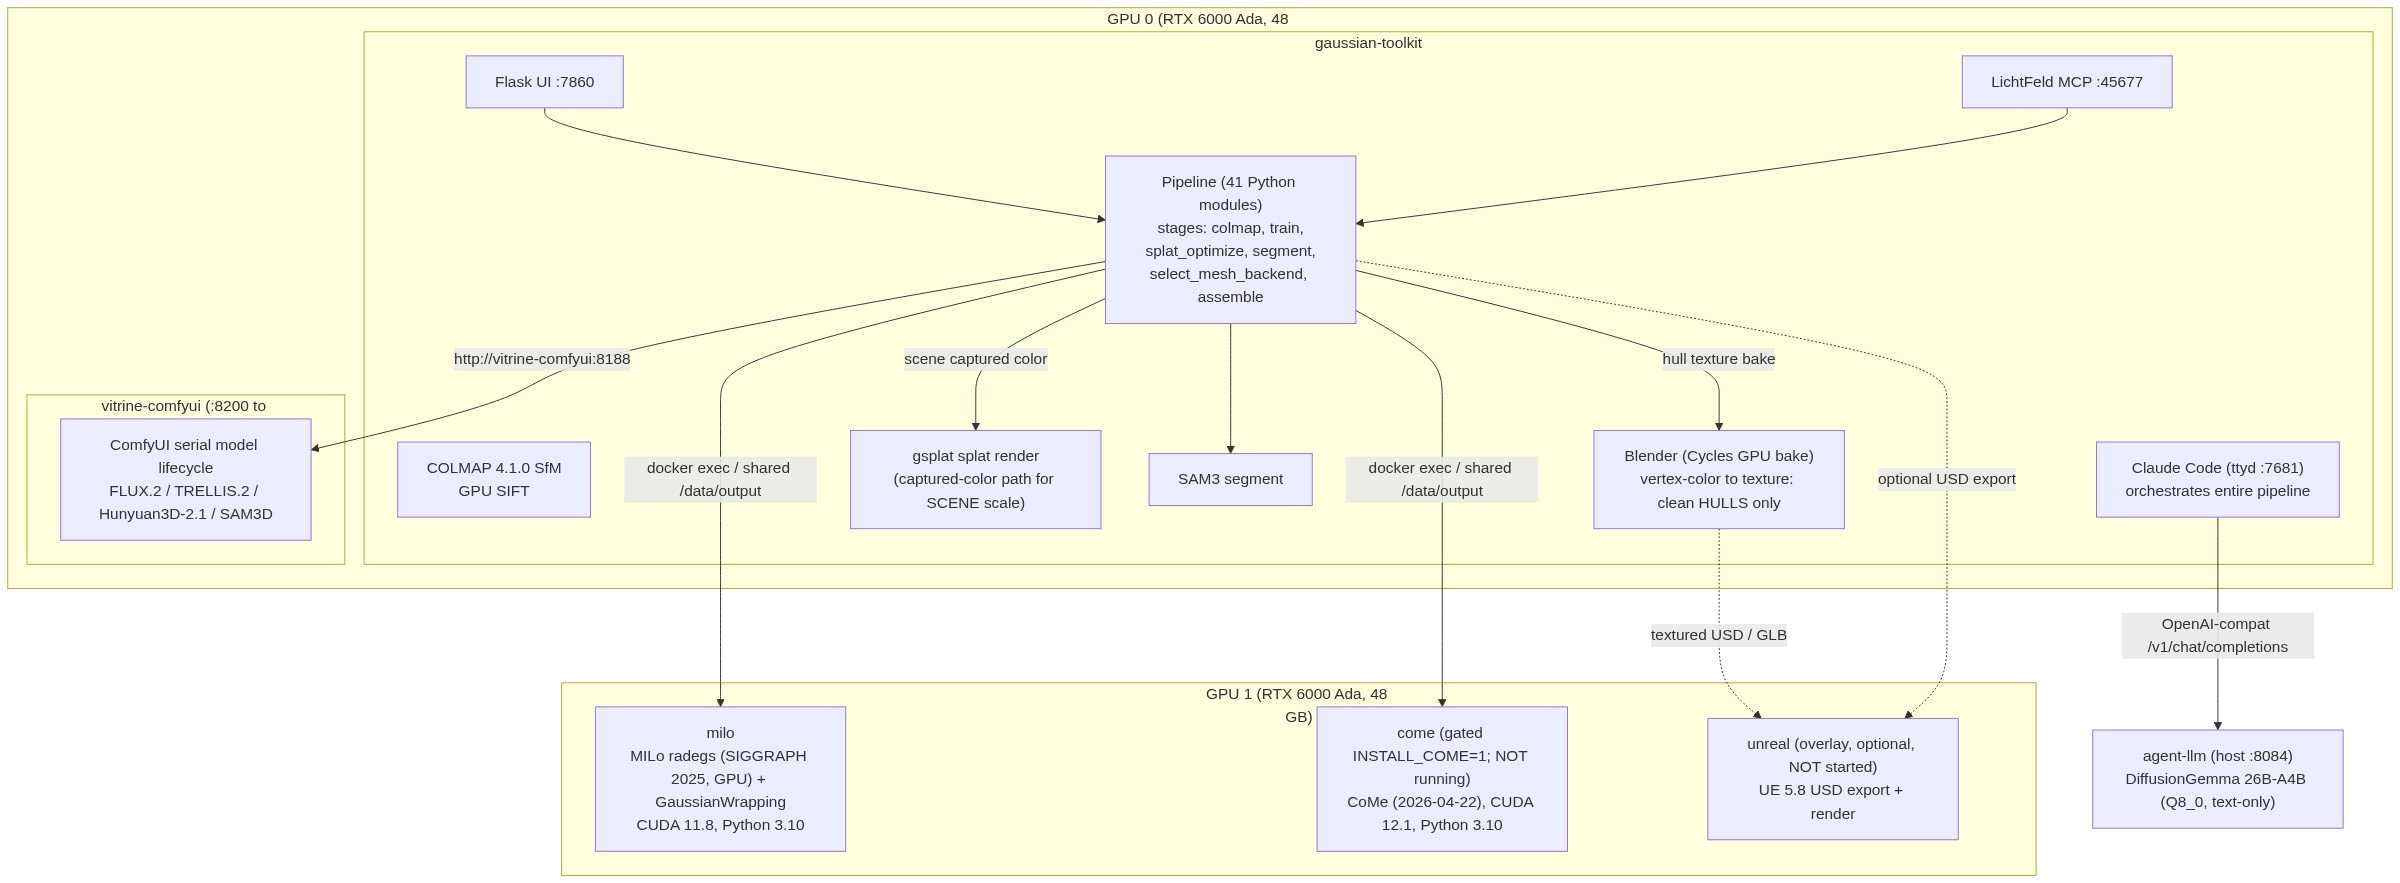
\includegraphics[width=\textwidth]{figures/architecture.jpg}
  \caption{%
    \textbf{Vitrine system architecture — Docker container topology.}
    Two RTX\,6000\,Ada GPUs (48\,GB each) host the six-container stack.
    GPU\,0 runs the \texttt{gaussian-toolkit} orchestrator (COLMAP, LichtFeld
    3DGS, SAM3, Flask\,UI, LichtFeld\,MCP on port\,45677) and
    \texttt{vitrine-comfyui} (FLUX.2\,/\,TRELLIS.2\,/\,Hunyuan3D-2.1, serial
    model lifecycle).
    GPU\,1 hosts the \texttt{milo} sidecar (MILo radegs, CUDA\,11.8) and the
    optional \texttt{come} (CoMe, CUDA\,12.1) and \texttt{unreal} (UE\,5.8)
    overlay containers.
    DiffusionGemma\,26B-A4B runs on the host at port\,8084 as the local text
    reasoner.
    All pipeline containers share \texttt{v2g-net}; the agentbox (Claude Code)
    reaches them via the shared \texttt{visionclaw\_network}.
  }
  \label{fig:architecture}
\end{figure}

% ──────────────────────────────────────────────────────────────────────────────
% 4. NanoGS room splat (docs canonical hero)
% ──────────────────────────────────────────────────────────────────────────────
\begin{figure}[htbp]
  \centering
  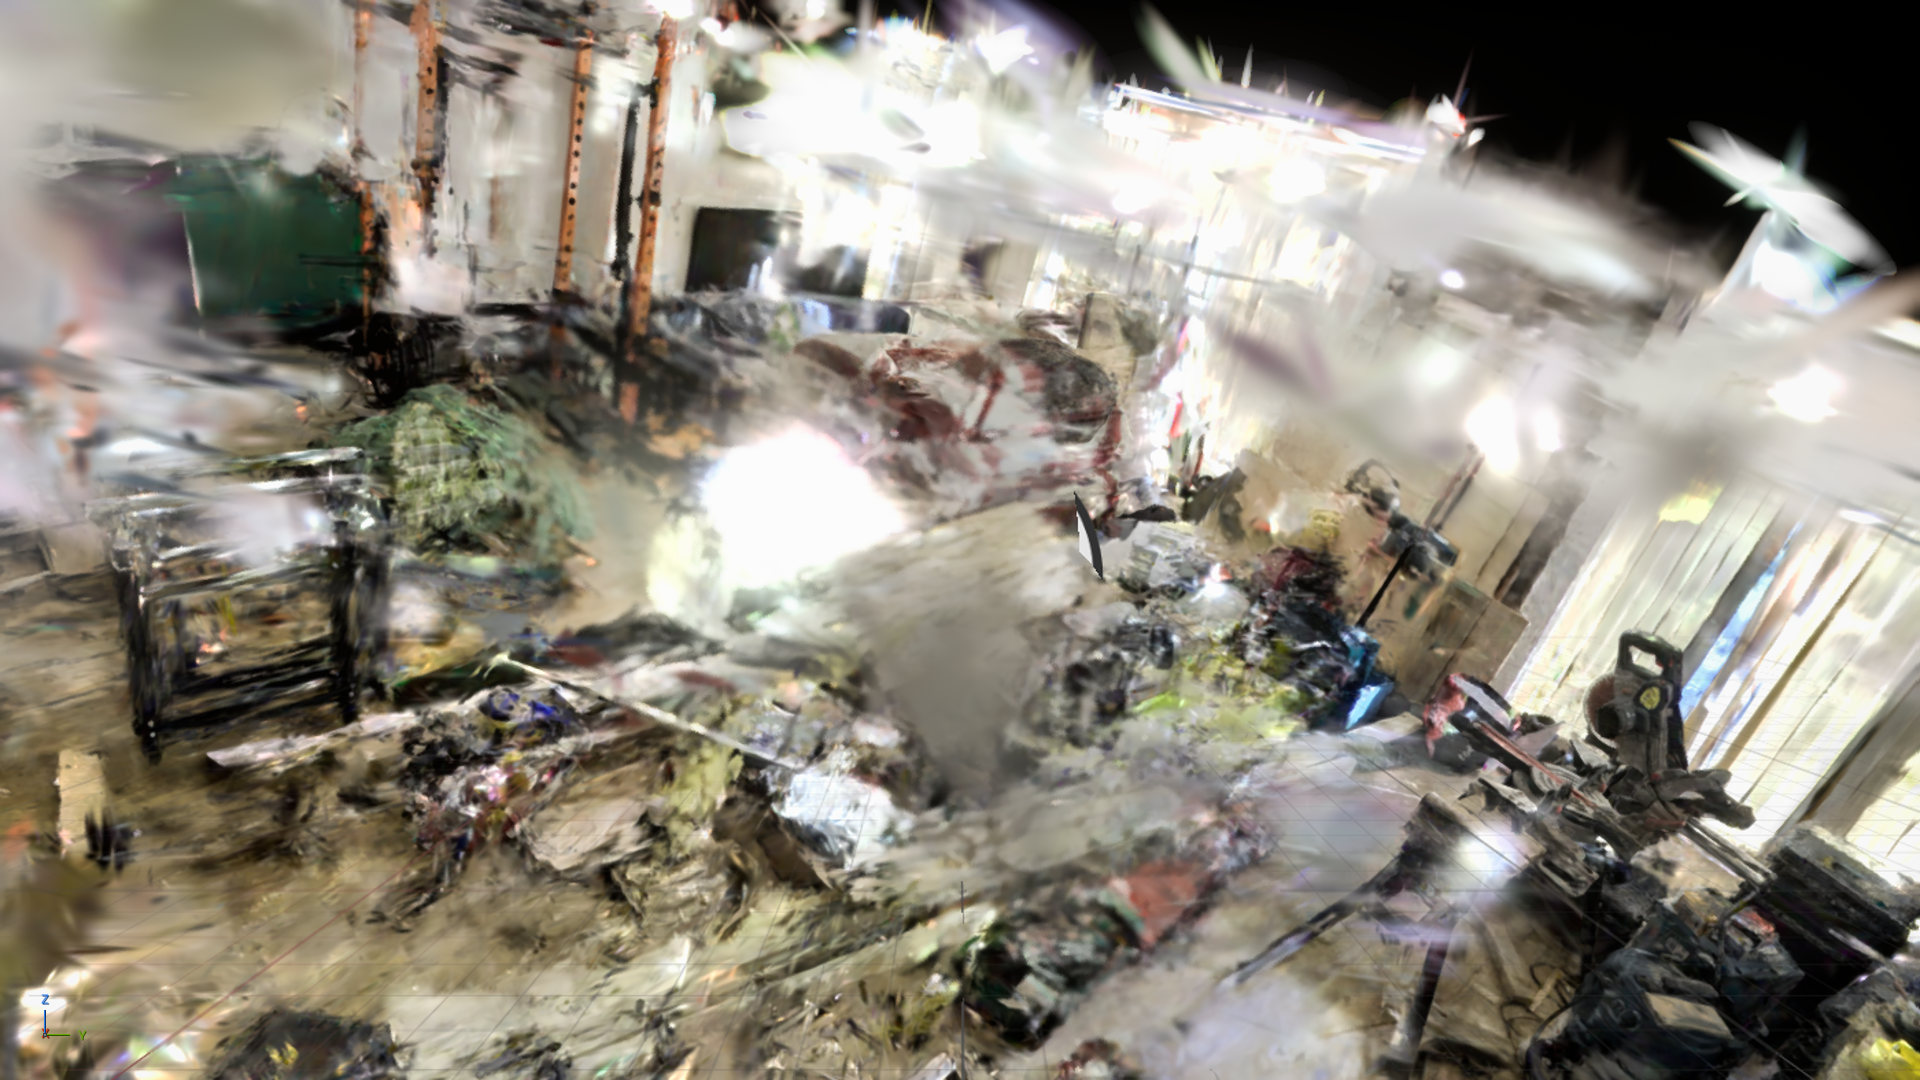
\includegraphics[width=\textwidth]{figures/nanogs_room_splat.png}
  \caption{%
    \textbf{Dreamlab room — NanoGS real-Gaussian splat render (canonical hero).}
    The LichtFeld-native \texttt{splat\_30000.ply}, cleaned via SuperSplat and
    loaded into the NanoGS\,(MIT) UE\,5.8 plugin, rendered at 1920$\times$1080.
    This replaces the earlier LiDAR point-cloud workaround and constitutes
    campaign step\,3: lean-on-LichtFeld native output for the room representation.
    Motion-blur softness in the source splat reflects the dreamlab capture
    constraint (MUSIQ $\approx$ 31); recapture at 4\,K\,/\,short shutter is the
    ceiling lever, not a pipeline limitation.
  }
  \label{fig:nanogs_room}
\end{figure}

% ──────────────────────────────────────────────────────────────────────────────
% 5. Fully integrated UE 5.8 scene
% ──────────────────────────────────────────────────────────────────────────────
\begin{figure}[htbp]
  \centering
  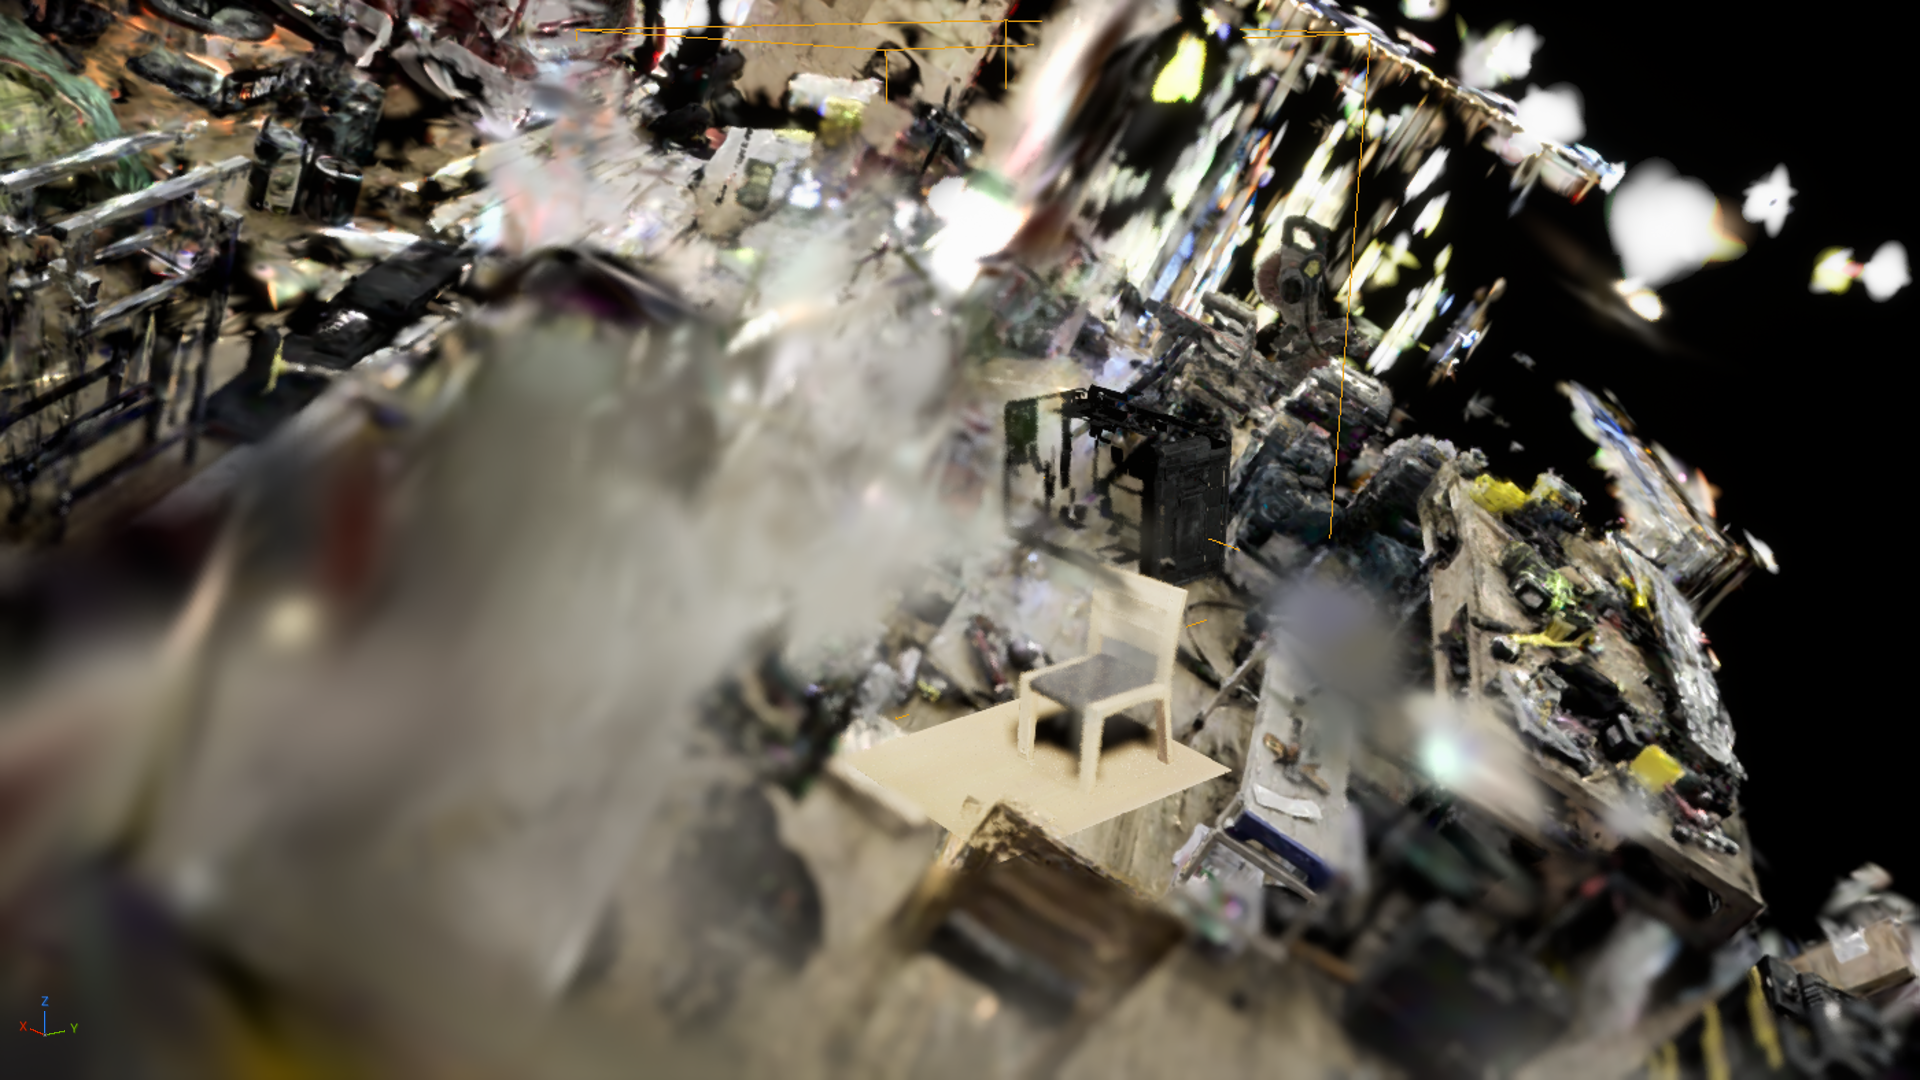
\includegraphics[width=\textwidth]{figures/scene_integrated.png}
  \caption{%
    \textbf{Integrated UE\,5.8 scene — room splat with placed TRELLIS.2 object FBXs.}
    The assembled deliverable: NanoGS splat room (hero representation) with
    chair, vacuum, and toolbox FBXs (TRELLIS.2 \texttt{hull\_e2e},
    prescaled via \texttt{blender\_prescale\_objects}) placed by
    \texttt{ue\_place\_prescaled}.
    Objects are Nanite game assets with baked PBR textures; the room splat
    renders real Gaussians.
    This image is the \emph{docs} canonical integrated-scene reference.
  }
  \label{fig:scene_integrated}
\end{figure}

% ──────────────────────────────────────────────────────────────────────────────
% 6. TRELLIS.2 object turnaround sheet (chair)
% ──────────────────────────────────────────────────────────────────────────────
\begin{figure}[htbp]
  \centering
  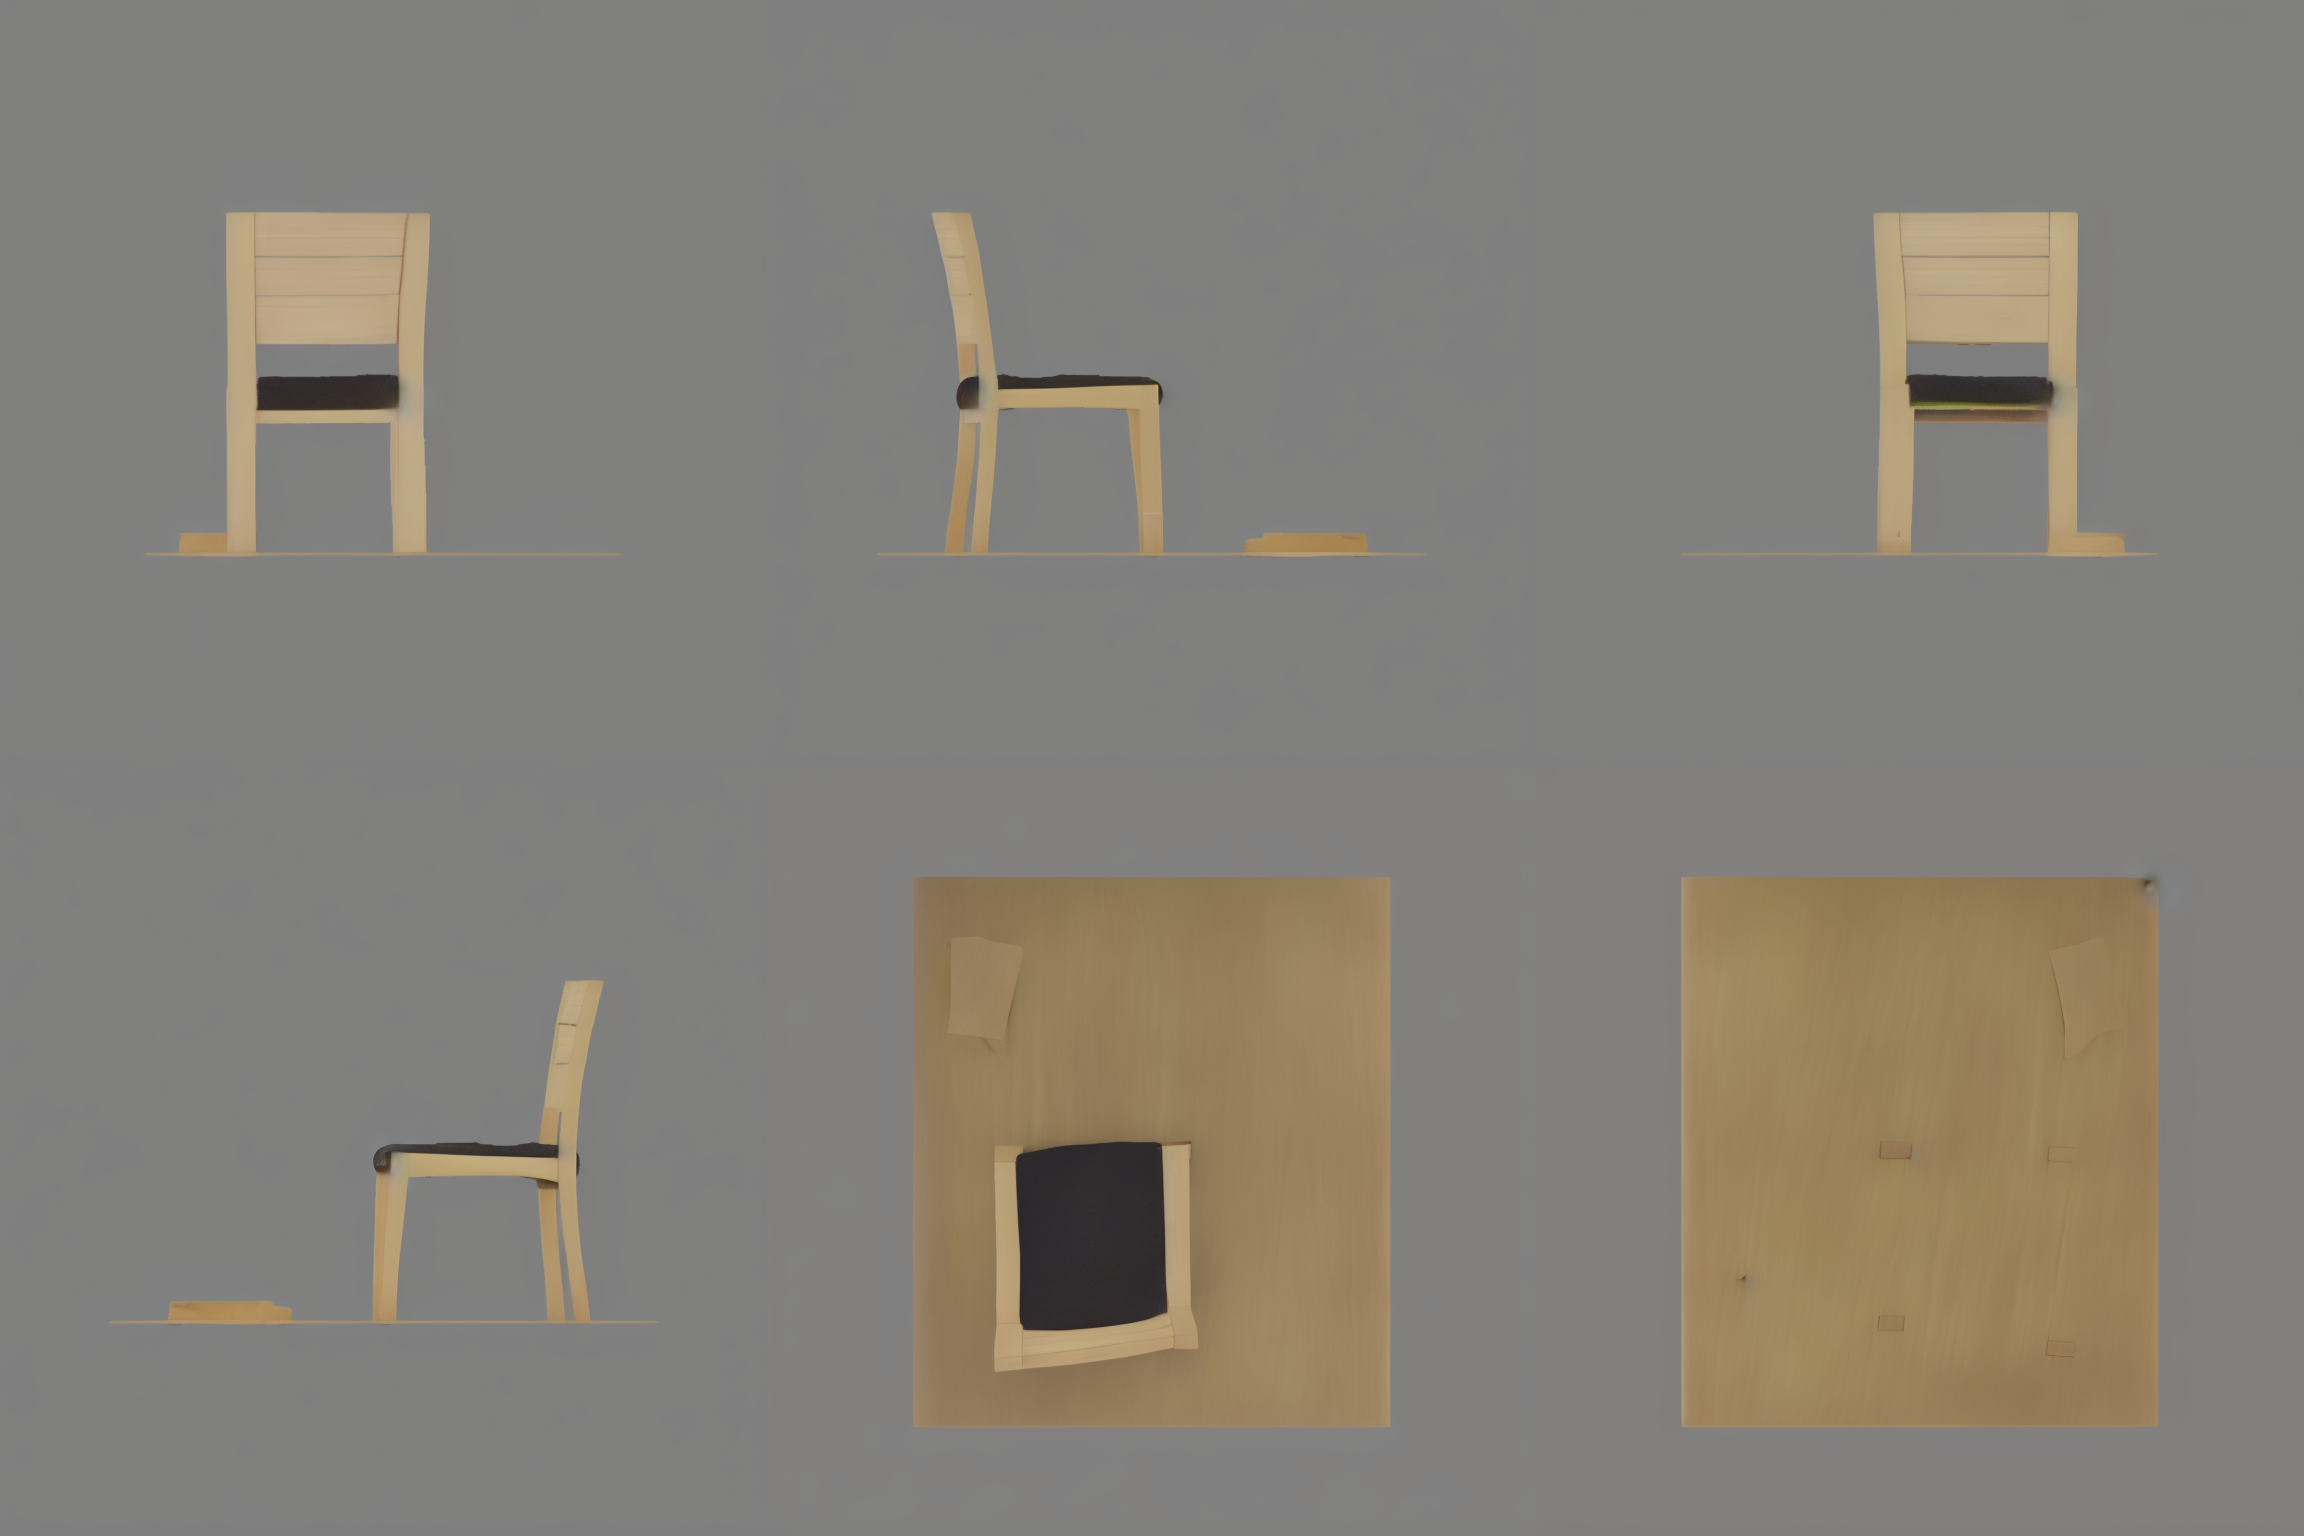
\includegraphics[width=\textwidth]{figures/chair_turnaround_sheet.png}
  \caption{%
    \textbf{TRELLIS.2 object reconstruction — chair turnaround sheet.}
    Multi-view orbit render of the textured GLB mesh produced by the
    \texttt{hull\_e2e} workflow: per-object SAM3 PLY crop $\to$ FLUX.2-dev
    view-inpainting $\to$ TRELLIS.2-4B mesh $\to$ PBR-baked GLB $\to$ FBX
    (Nanite game asset).
    The chair is rated \emph{good}; vacuum and toolbox likewise passed
    the object reconstruction gate (4/8 objects in this batch).
    Resolution: 2304$\times$1536.
  }
  \label{fig:objects}
\end{figure}

% ──────────────────────────────────────────────────────────────────────────────
% 7. CoMe-TSDF mesh in UE (baseline mesh deliverable)
% ──────────────────────────────────────────────────────────────────────────────
\begin{figure}[htbp]
  \centering
  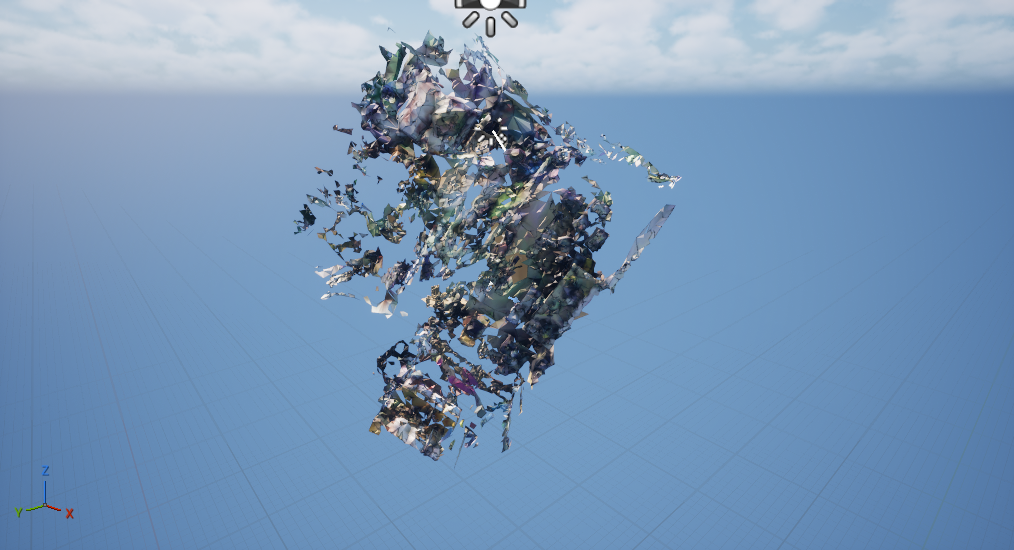
\includegraphics[width=\textwidth]{figures/ue_come_final.png}
  \caption{%
    \textbf{CoMe-TSDF room mesh game asset in UE\,5.8 (baseline mesh deliverable).}
    The scene-mesh branch: CoMe legacy \texttt{ScalableTSDFVolume} extraction,
    \texttt{mesh\_cleaner} (smooth=0, edge-length + connected-component cleanup),
    xatlas bake (\texttt{bake\_from\_vertex\_colors}), \texttt{blender\_obj\_to\_fbx},
    imported as a Nanite mesh.
    Characteristic TSDF blockiness on flat walls is visible; this image
    motivates the re-spine to NanoGS as the default room representation for
    blur-limited captures.
    Resolution: 1014$\times$550.
  }
  \label{fig:ue_come}
\end{figure}

% ──────────────────────────────────────────────────────────────────────────────
% 8. NanoGS splat render (1920×1080 B-view)
% ──────────────────────────────────────────────────────────────────────────────
\begin{figure}[htbp]
  \centering
  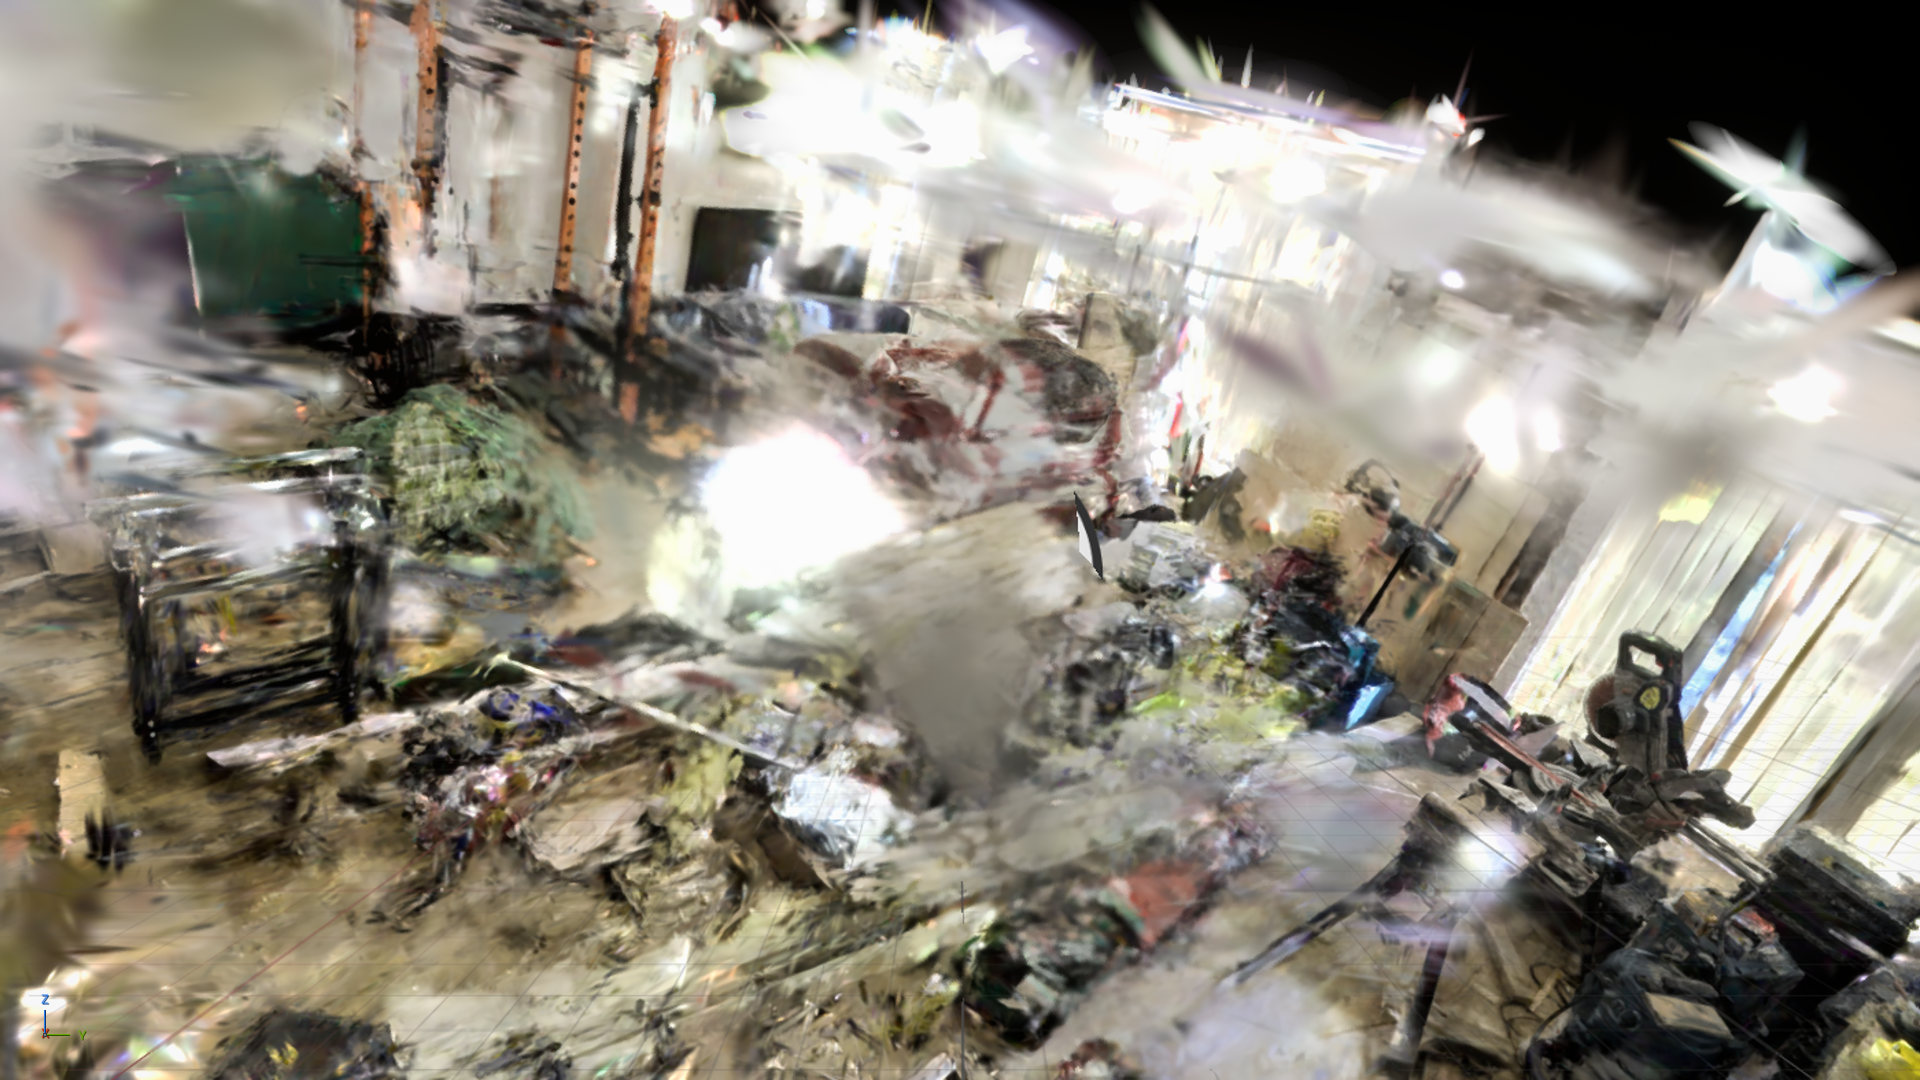
\includegraphics[width=\textwidth]{figures/ue_nanogs_room_B.png}
  \caption{%
    \textbf{NanoGS real-Gaussian splat in UE\,5.8 — interior view (B).}
    Second viewpoint of the NanoGS splat room, demonstrating depth and
    parallax of real Gaussian rendering at 1920$\times$1080.
    Comparison with Figure~\ref{fig:ue_come} illustrates the quality
    improvement of splat-hero over TSDF mesh for a motion-blur-limited
    capture: the splat faithfully preserves captured radiance;
    the mesh introduces geometric artefacts irrelevant to the capture.
  }
  \label{fig:ue_nanogs}
\end{figure}

% ──────────────────────────────────────────────────────────────────────────────
% 9. Hero perspective render (room + placed objects)
% ──────────────────────────────────────────────────────────────────────────────
\begin{figure}[htbp]
  \centering
  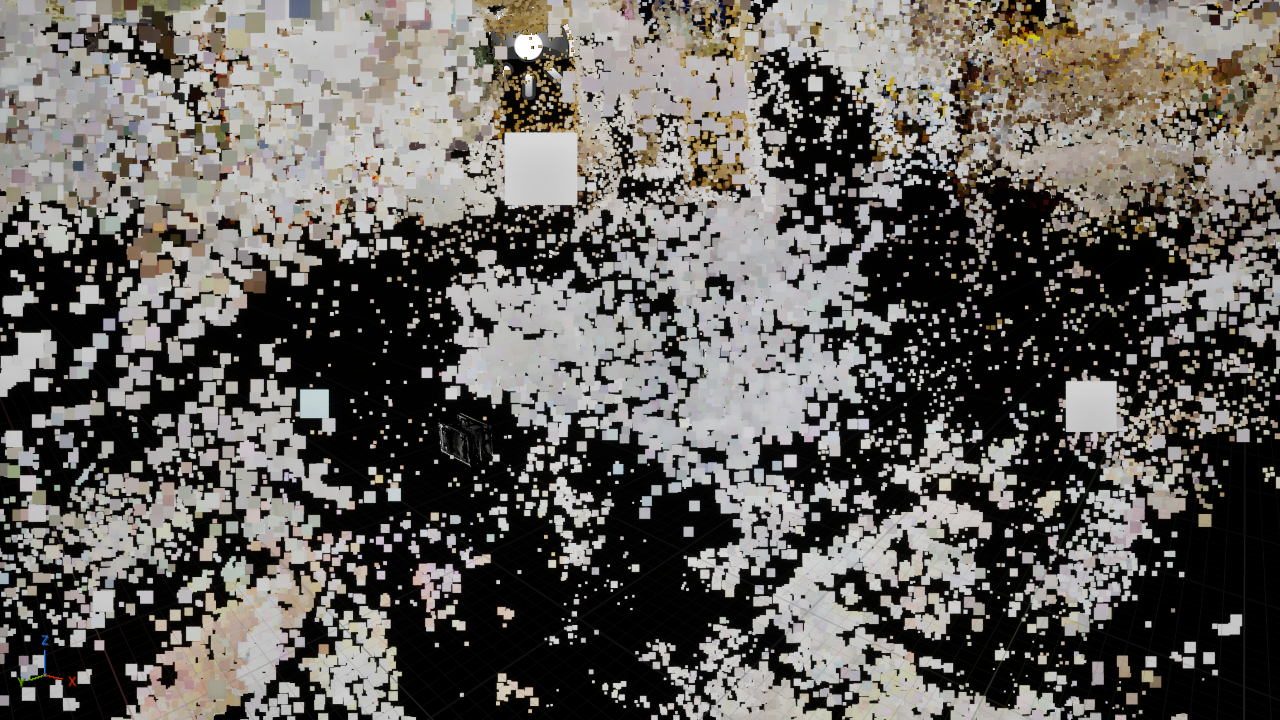
\includegraphics[width=\textwidth]{figures/ue_final_hero.png}
  \caption{%
    \textbf{Hero perspective render — dreamlab room with placed object FBXs.}
    A cinematic view of the assembled UE\,5.8 scene from the validated
    end-to-end run (2026-06-22): TSDF-mesh room (CoMe, pre-NanoGS re-spine)
    with TRELLIS.2 object FBXs placed by \texttt{ue\_place\_prescaled}.
    Resolution: 1280$\times$720.
    Serves as the primary before/after reference for evaluating the
    NanoGS re-spine (Figure~\ref{fig:nanogs_room}).
  }
  \label{fig:ue_hero}
\end{figure}

% ──────────────────────────────────────────────────────────────────────────────
% 10. Overhead dollhouse view
% ──────────────────────────────────────────────────────────────────────────────
\begin{figure}[htbp]
  \centering
  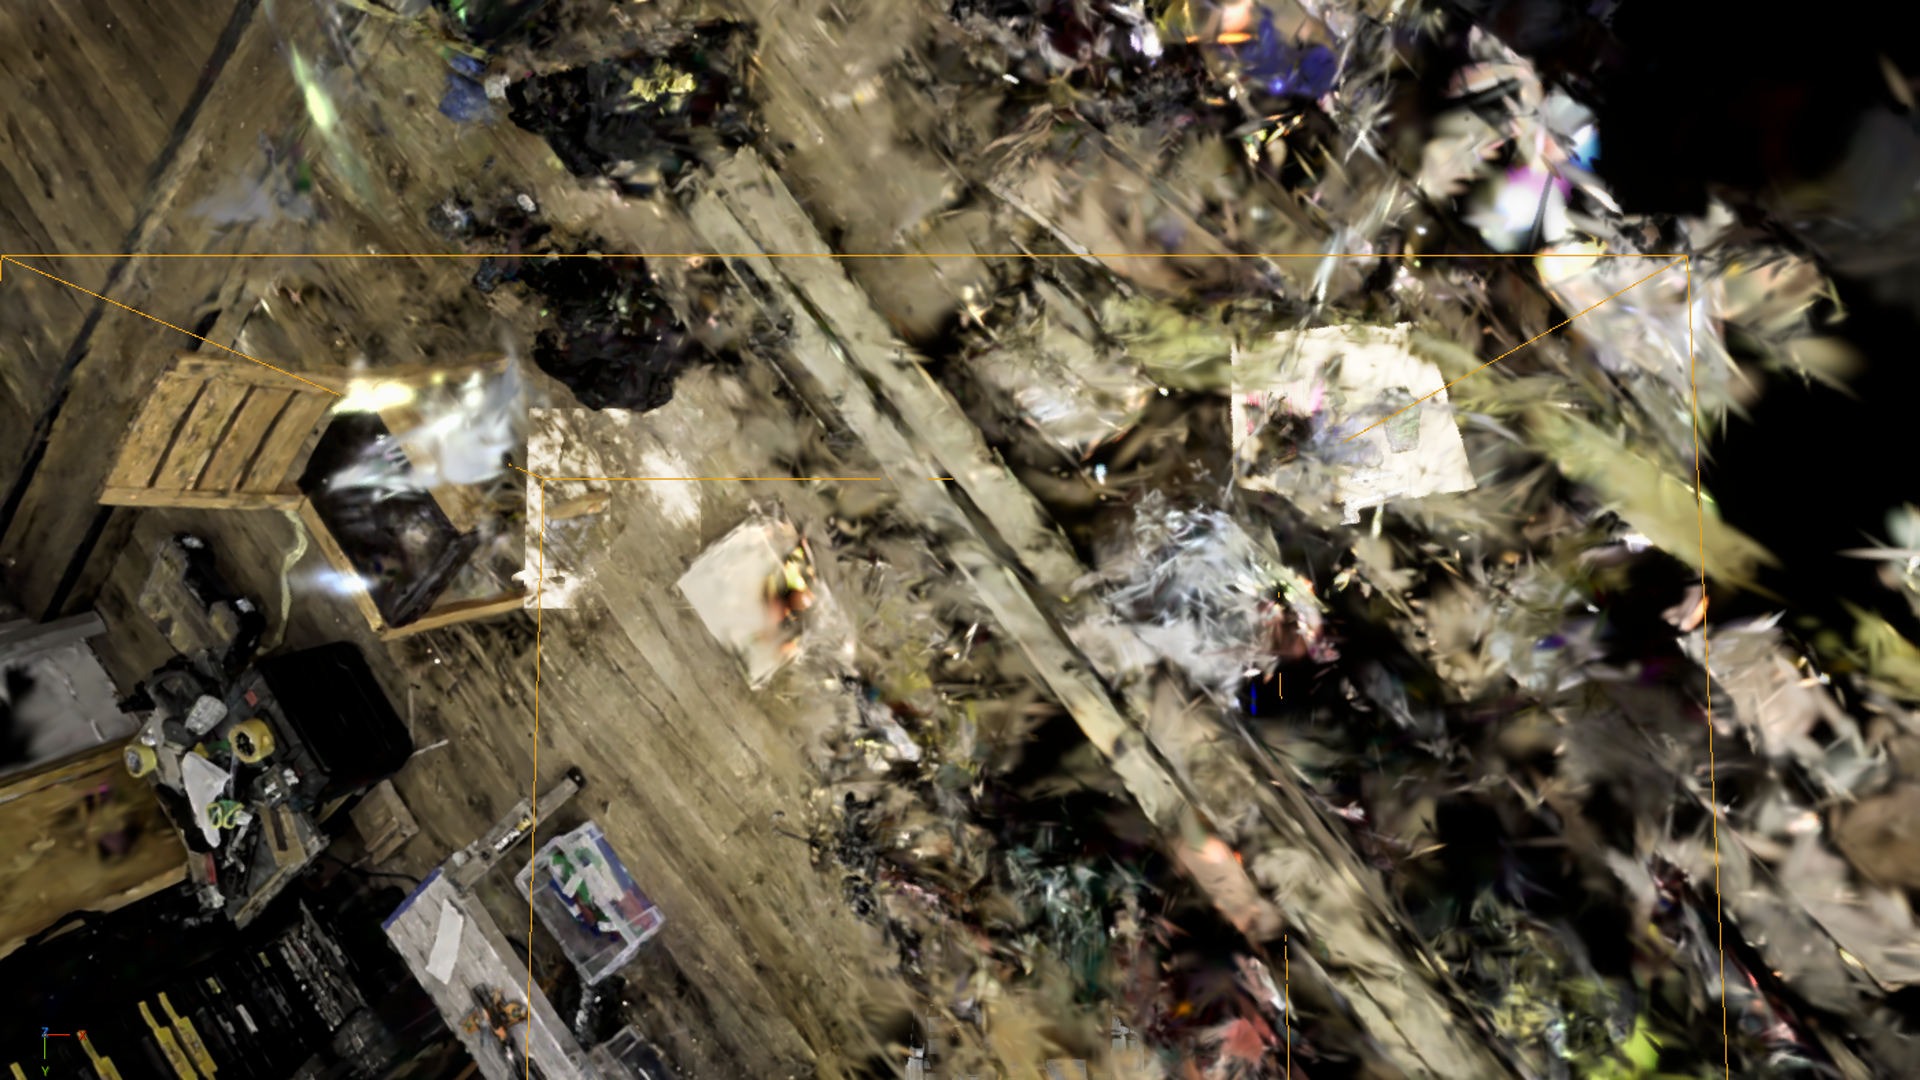
\includegraphics[width=\textwidth]{figures/ue_integrated_dollhouse.png}
  \caption{%
    \textbf{Overhead dollhouse view — integrated UE\,5.8 scene layout.}
    Top-down perspective revealing object placement, room geometry, and
    spatial relationships of the dreamlab scene.
    The dollhouse view is the standard QA checkpoint for scale fidelity
    and object-in-room alignment after \texttt{ue\_place\_prescaled}
    prescaling.
    Resolution: 1920$\times$1080.
  }
  \label{fig:ue_dollhouse}
\end{figure}

% Assumes \graphicspath{{figures/}} is set in the preamble (relative to report/v5/).
%
% Labels (for \ref / \autoref):
%   fig:router           — capture-adaptive router flowchart
%   fig:component_menu   — component-menu status flowchart
%   fig:architecture     — system architecture (container topology)
%   fig:nanogs_room      — NanoGS real-Gaussian splat render (canonical room hero)
%   fig:scene_integrated — fully integrated UE 5.8 scene (room + objects)
%   fig:objects          — TRELLIS.2 object turnaround sheet (chair)
%   fig:ue_come          — CoMe-TSDF mesh game asset in UE (baseline mesh)
%   fig:ue_nanogs        — NanoGS splat render (dreamlab room, 1920x1080)
%   fig:ue_hero          — Hero perspective render (room + placed objects)
%   fig:ue_dollhouse     — Overhead dollhouse view of integrated UE scene

% ──────────────────────────────────────────────────────────────────────────────
% 1. Capture-adaptive router
% ──────────────────────────────────────────────────────────────────────────────
\begin{figure}[htbp]
  \centering
  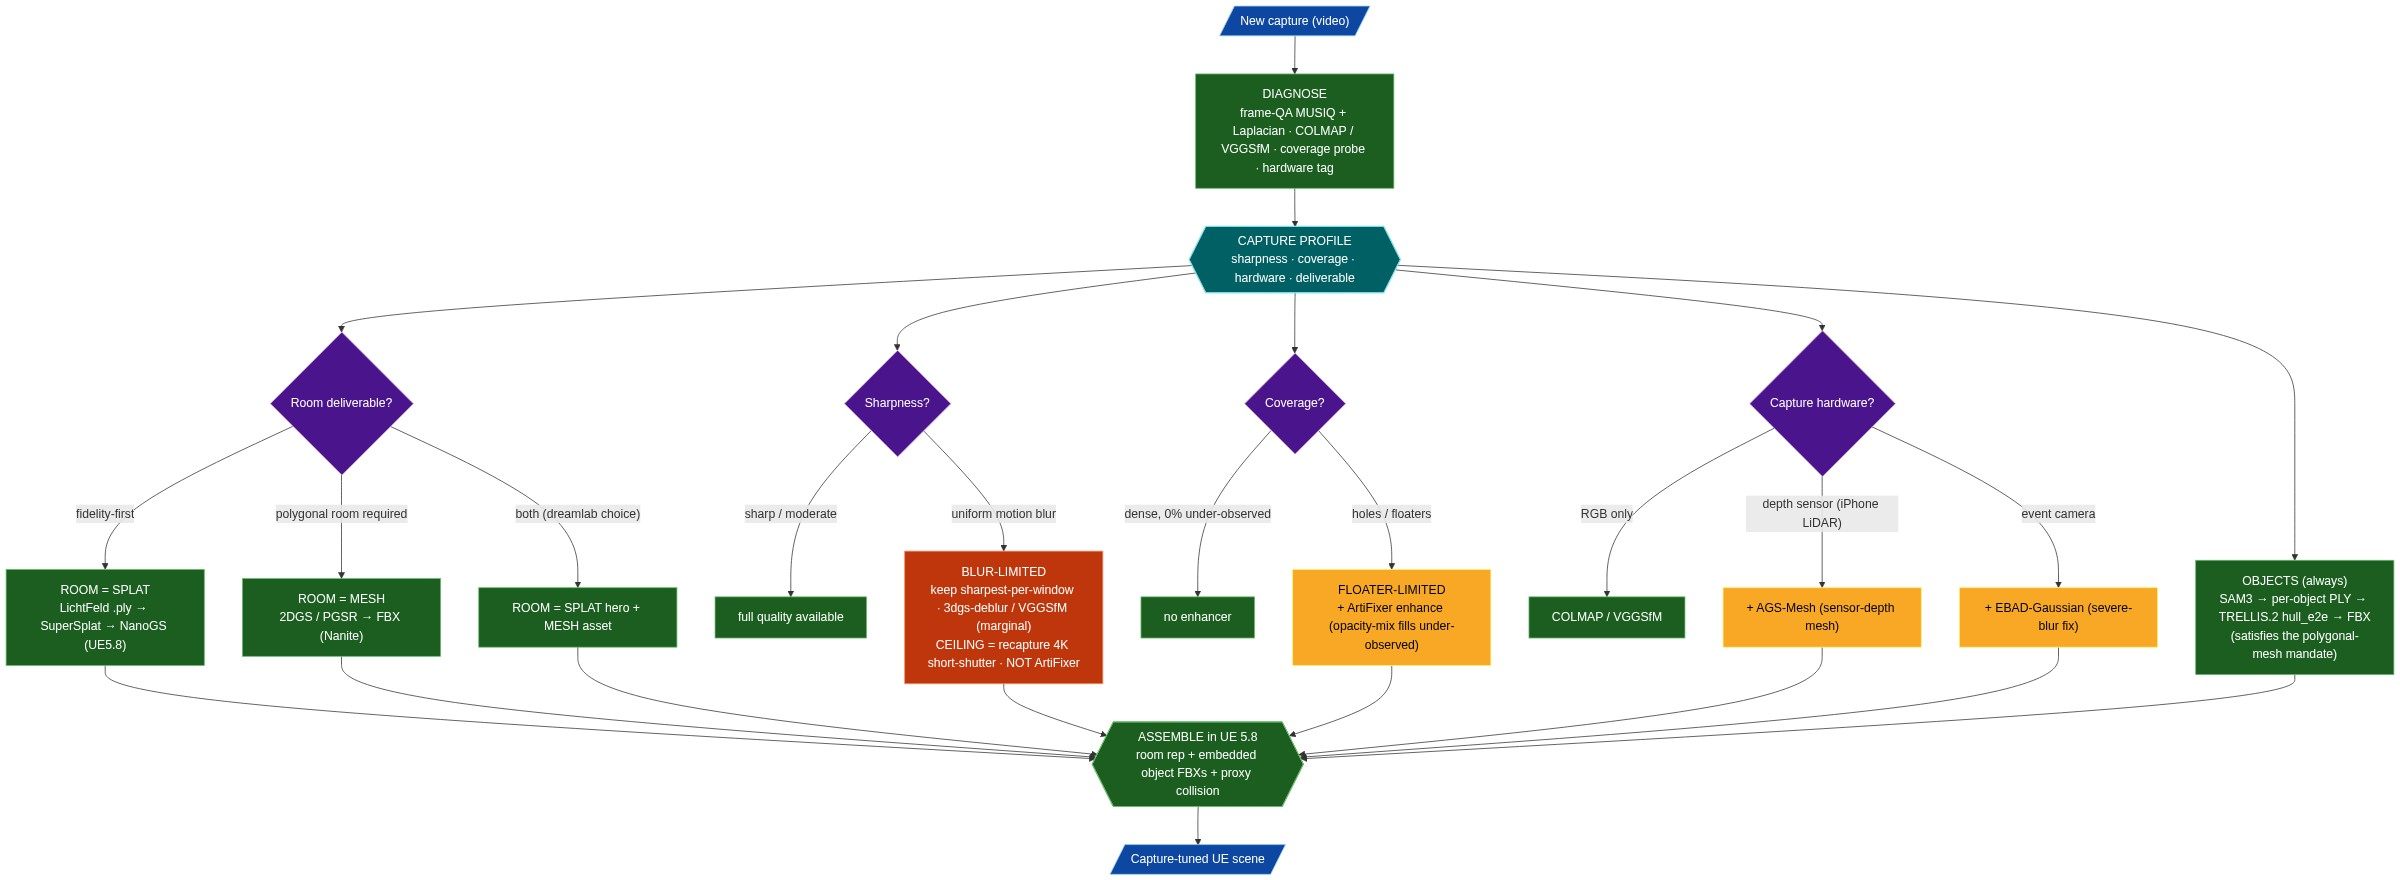
\includegraphics[width=\textwidth]{figures/router.jpg}
  \caption{%
    \textbf{Capture-adaptive router.}
    The pipeline diagnoses each new capture on four axes
    (sharpness via MUSIQ + full-resolution Laplacian, coverage via occupancy probe,
    available hardware, and deliverable type) and selects the configuration that
    fits the bottleneck.
    Green nodes are validated keepers; orange nodes are
    capture-conditional options; red nodes are blur-limited warnings.
    The dreamlab capture routes to Opt\,4 (splat hero + mesh asset + TRELLIS.2 objects)
    with a recapture flag as the quality ceiling.
  }
  \label{fig:router}
\end{figure}

% ──────────────────────────────────────────────────────────────────────────────
% 2. Component-menu flowchart
% ──────────────────────────────────────────────────────────────────────────────
\begin{figure}[htbp]
  \centering
  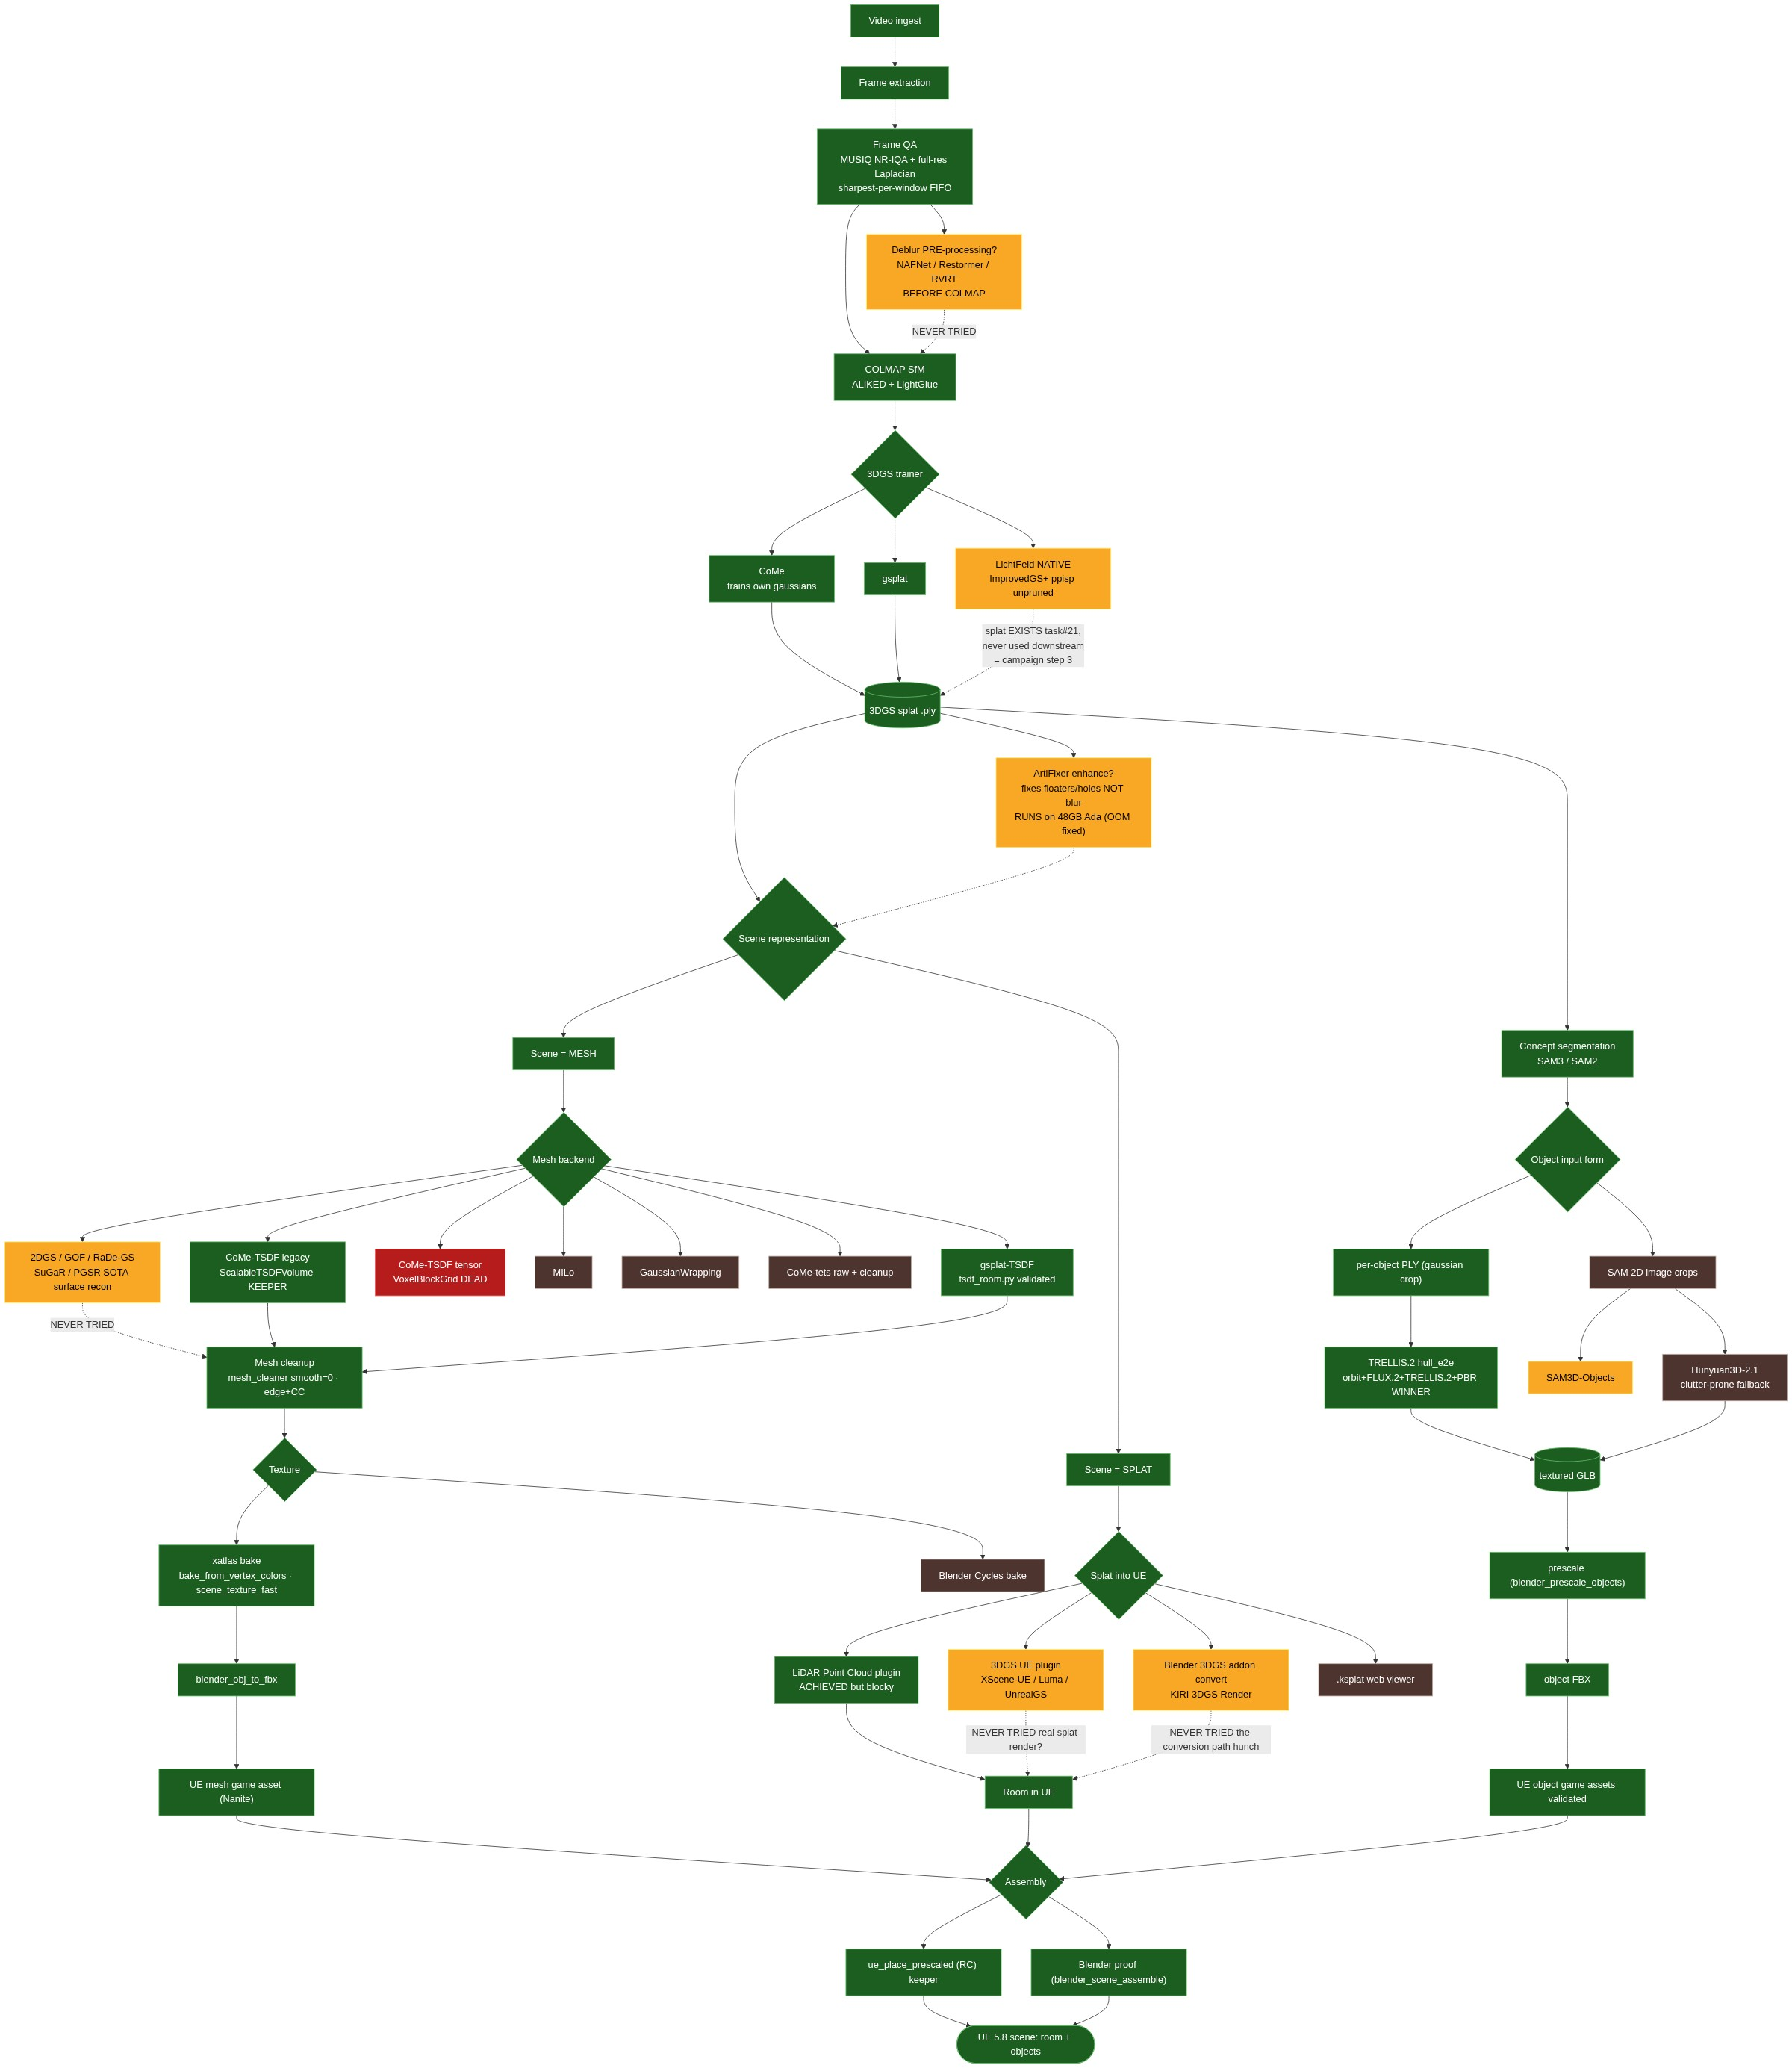
\includegraphics[width=\textwidth]{figures/component_menu.jpg}
  \caption{%
    \textbf{Full component-menu status chart (validated 2026-06-25).}
    Every branch of the Vitrine toolkit from video ingest to UE\,5.8 delivery.
    Colour coding: \emph{green} = validated keeper in active use;
    \emph{brown} = exercised but subordinate / fallback;
    \emph{red} = tried and abandoned;
    \emph{yellow} = plausible, never run.
    The chart is the canonical record of what has and has not been exercised;
    dashed arrows mark paths that remain open research items
    (SAM3D-Objects, BAD-Gaussians deblur, PGSR/2DGS surface reconstruction).
  }
  \label{fig:component_menu}
\end{figure}

% ──────────────────────────────────────────────────────────────────────────────
% 3. System architecture (container topology)
% ──────────────────────────────────────────────────────────────────────────────
\begin{figure}[htbp]
  \centering
  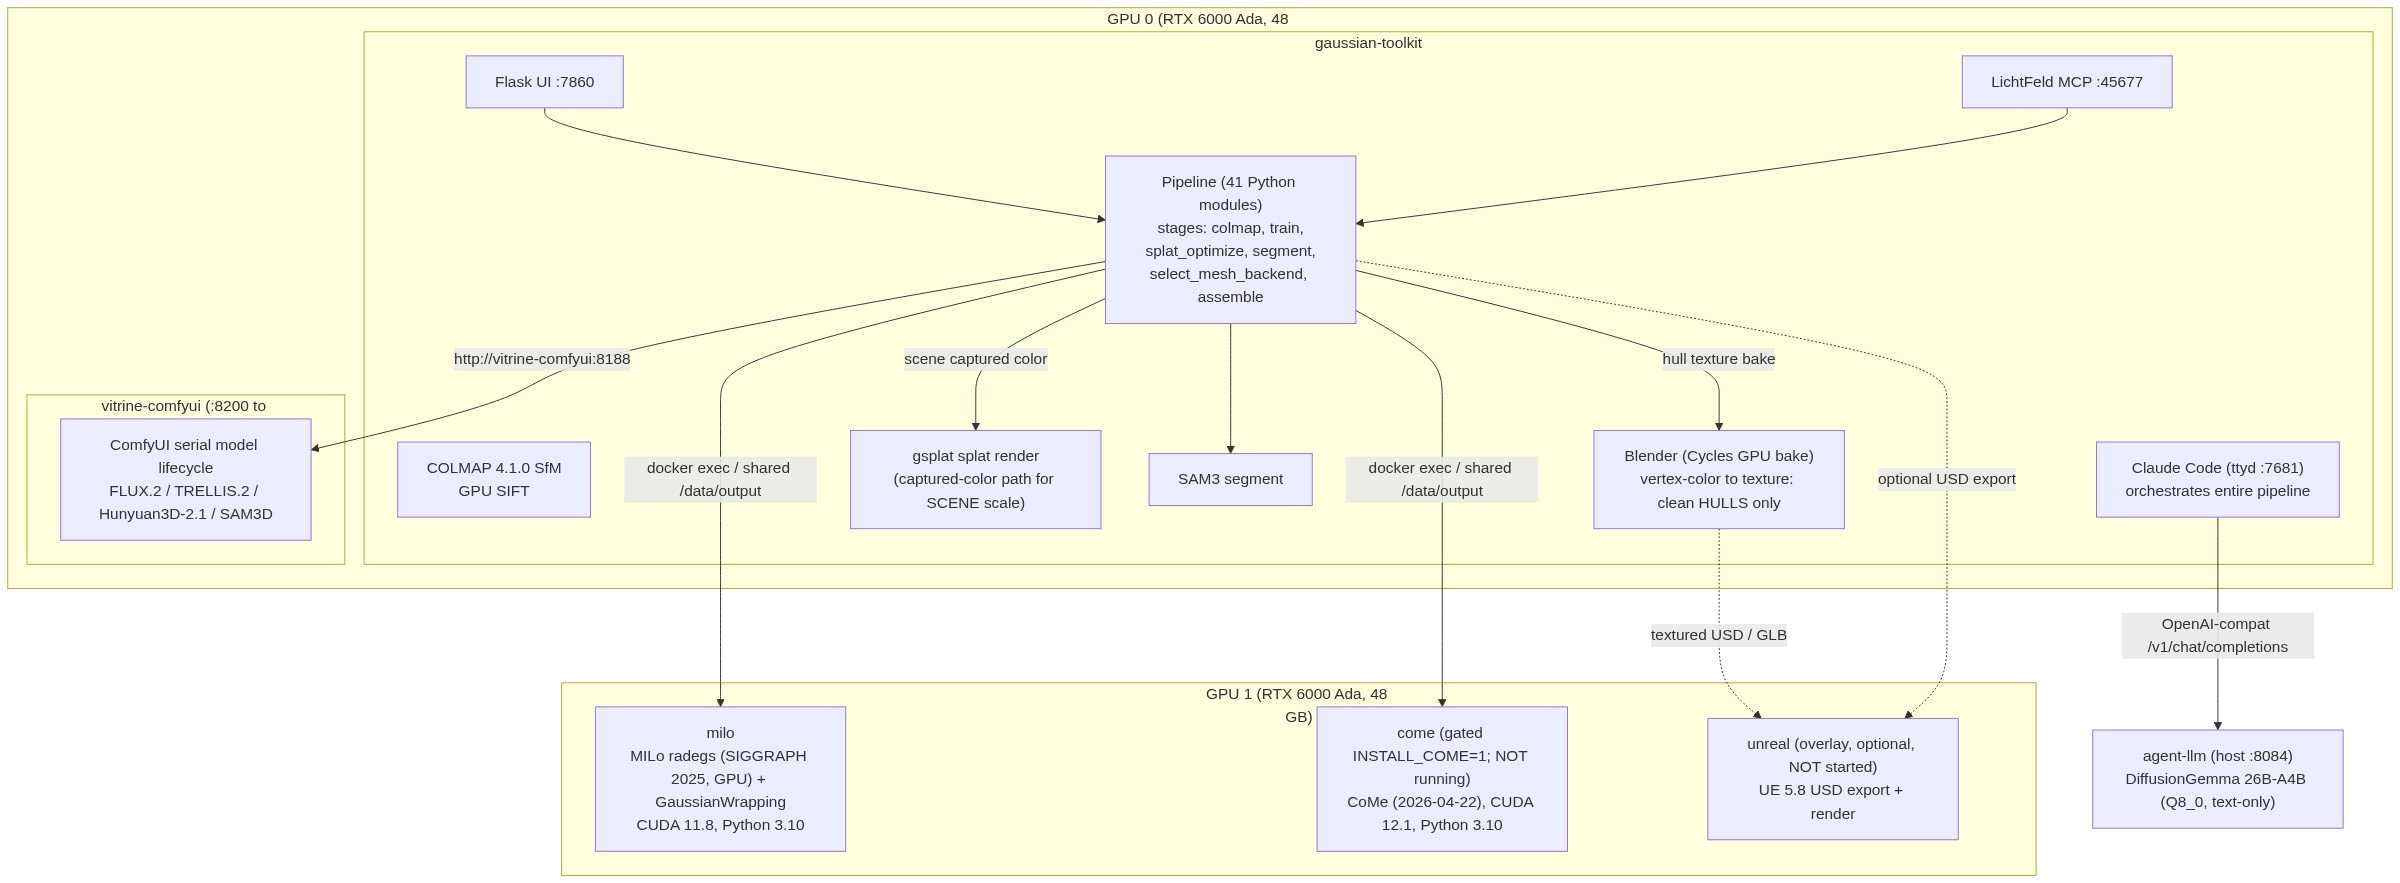
\includegraphics[width=\textwidth]{figures/architecture.jpg}
  \caption{%
    \textbf{Vitrine system architecture — Docker container topology.}
    Two RTX\,6000\,Ada GPUs (48\,GB each) host the six-container stack.
    GPU\,0 runs the \texttt{gaussian-toolkit} orchestrator (COLMAP, LichtFeld
    3DGS, SAM3, Flask\,UI, LichtFeld\,MCP on port\,45677) and
    \texttt{vitrine-comfyui} (FLUX.2\,/\,TRELLIS.2\,/\,Hunyuan3D-2.1, serial
    model lifecycle).
    GPU\,1 hosts the \texttt{milo} sidecar (MILo radegs, CUDA\,11.8) and the
    optional \texttt{come} (CoMe, CUDA\,12.1) and \texttt{unreal} (UE\,5.8)
    overlay containers.
    DiffusionGemma\,26B-A4B runs on the host at port\,8084 as the local text
    reasoner.
    All pipeline containers share \texttt{v2g-net}; the agentbox (Claude Code)
    reaches them via the shared \texttt{visionclaw\_network}.
  }
  \label{fig:architecture}
\end{figure}

% ──────────────────────────────────────────────────────────────────────────────
% 4. NanoGS room splat (docs canonical hero)
% ──────────────────────────────────────────────────────────────────────────────
\begin{figure}[htbp]
  \centering
  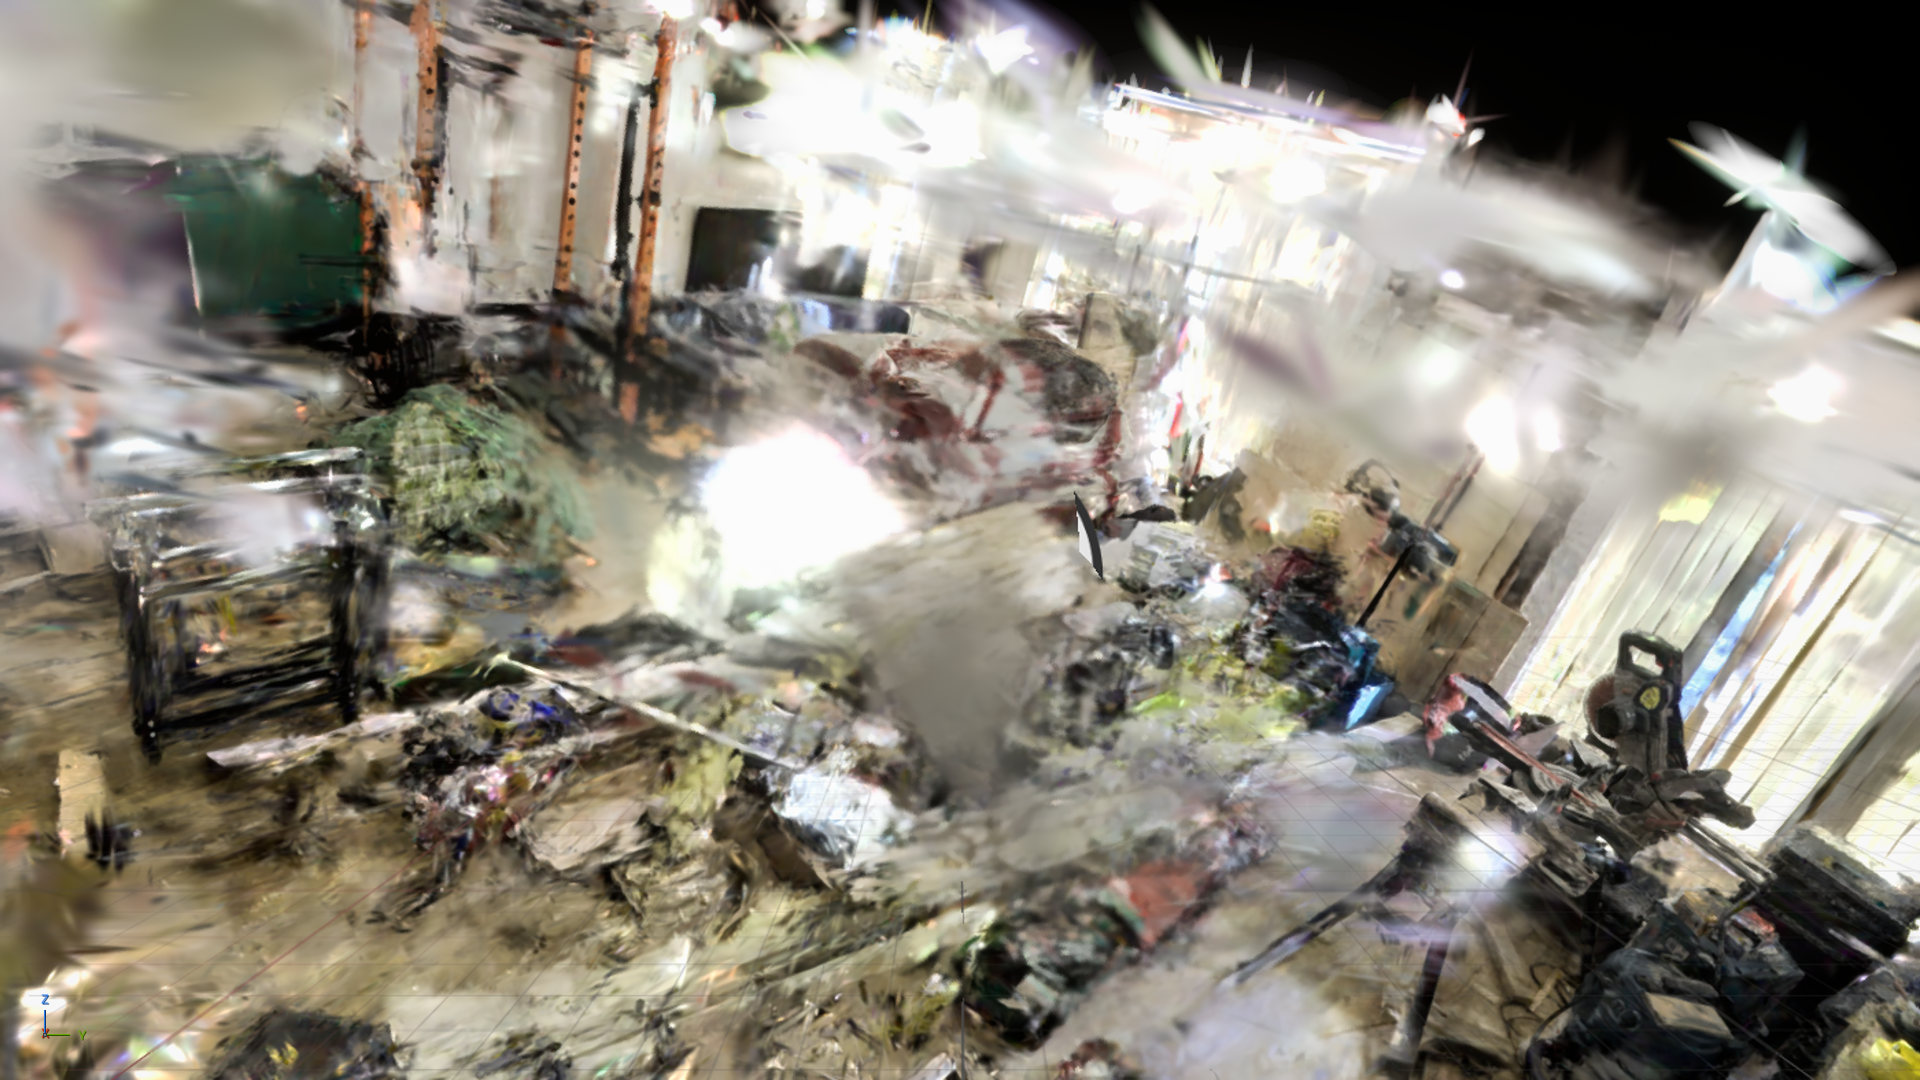
\includegraphics[width=\textwidth]{figures/nanogs_room_splat.png}
  \caption{%
    \textbf{Dreamlab room — NanoGS real-Gaussian splat render (canonical hero).}
    The LichtFeld-native \texttt{splat\_30000.ply}, cleaned via SuperSplat and
    loaded into the NanoGS\,(MIT) UE\,5.8 plugin, rendered at 1920$\times$1080.
    This replaces the earlier LiDAR point-cloud workaround and constitutes
    campaign step\,3: lean-on-LichtFeld native output for the room representation.
    Motion-blur softness in the source splat reflects the dreamlab capture
    constraint (MUSIQ $\approx$ 31); recapture at 4\,K\,/\,short shutter is the
    ceiling lever, not a pipeline limitation.
  }
  \label{fig:nanogs_room}
\end{figure}

% ──────────────────────────────────────────────────────────────────────────────
% 5. Fully integrated UE 5.8 scene
% ──────────────────────────────────────────────────────────────────────────────
\begin{figure}[htbp]
  \centering
  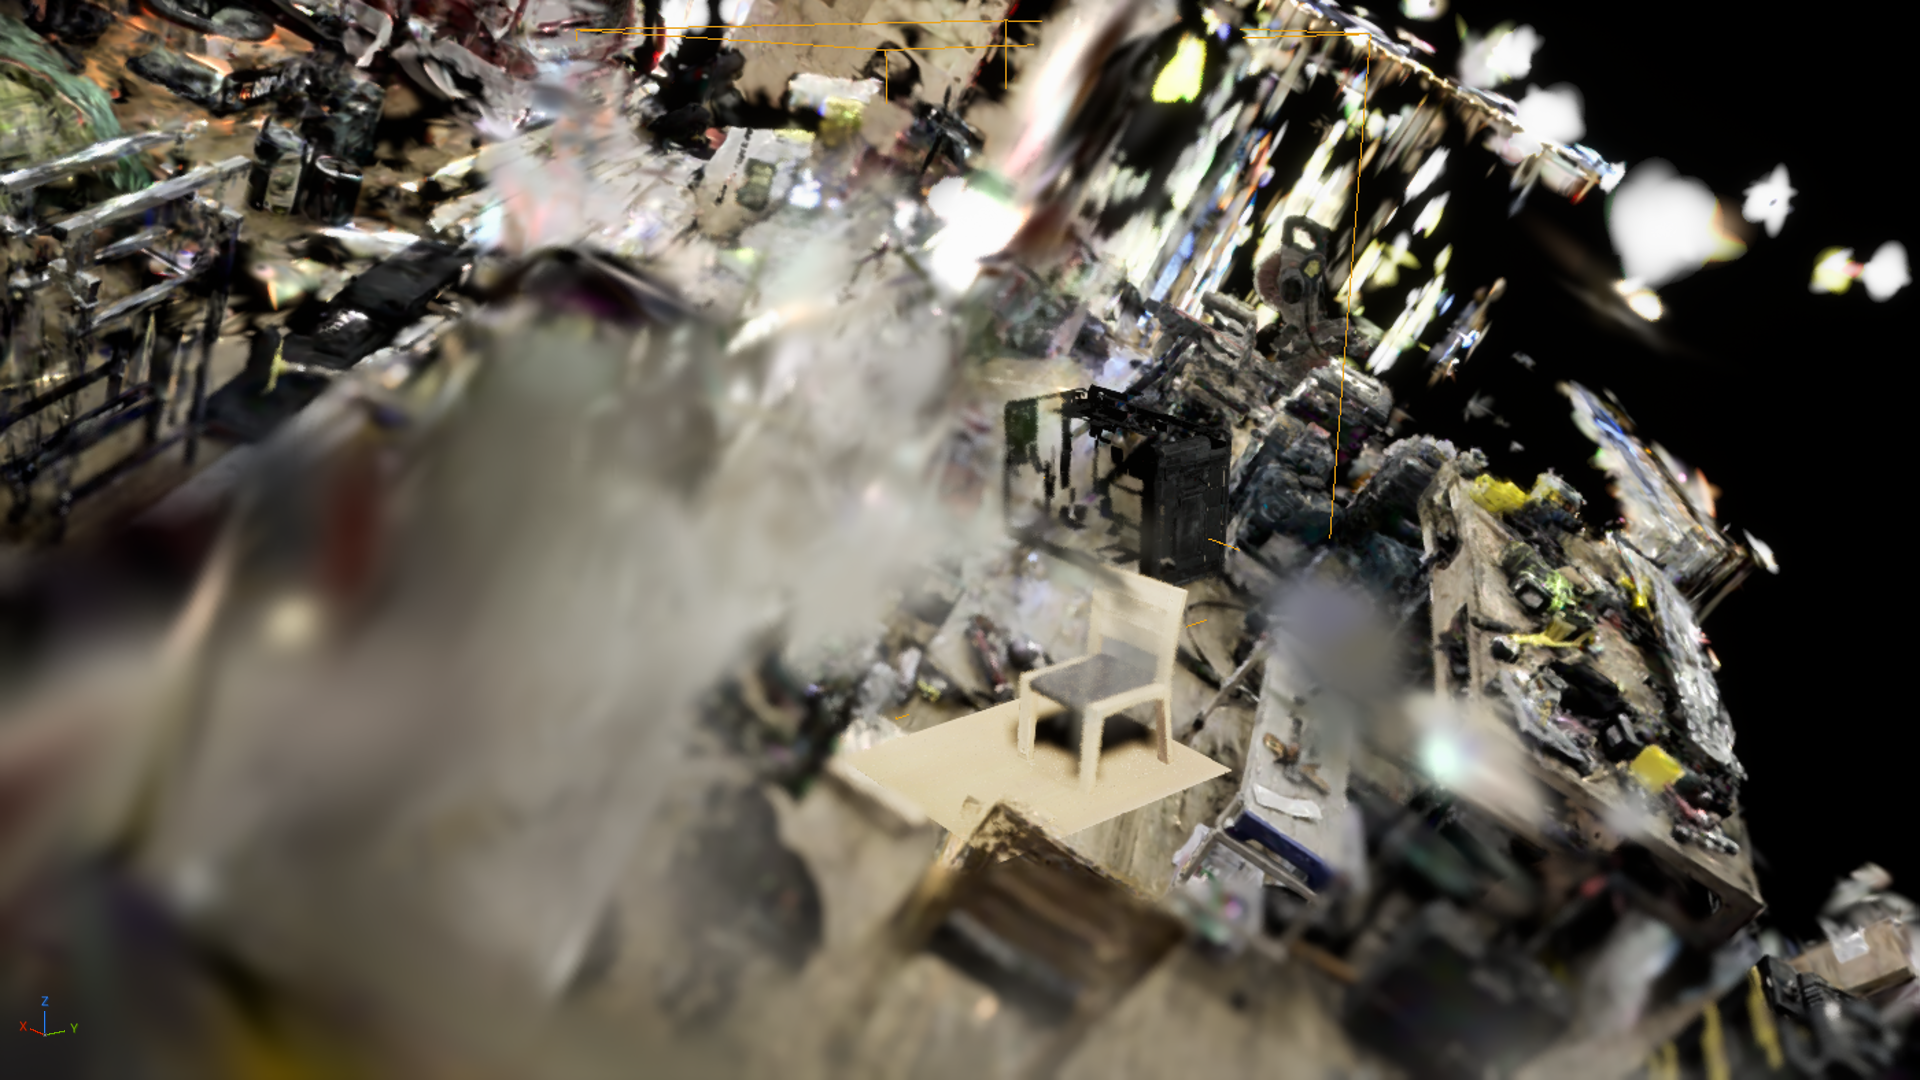
\includegraphics[width=\textwidth]{figures/scene_integrated.png}
  \caption{%
    \textbf{Integrated UE\,5.8 scene — room splat with placed TRELLIS.2 object FBXs.}
    The assembled deliverable: NanoGS splat room (hero representation) with
    chair, vacuum, and toolbox FBXs (TRELLIS.2 \texttt{hull\_e2e},
    prescaled via \texttt{blender\_prescale\_objects}) placed by
    \texttt{ue\_place\_prescaled}.
    Objects are Nanite game assets with baked PBR textures; the room splat
    renders real Gaussians.
    This image is the \emph{docs} canonical integrated-scene reference.
  }
  \label{fig:scene_integrated}
\end{figure}

% ──────────────────────────────────────────────────────────────────────────────
% 6. TRELLIS.2 object turnaround sheet (chair)
% ──────────────────────────────────────────────────────────────────────────────
\begin{figure}[htbp]
  \centering
  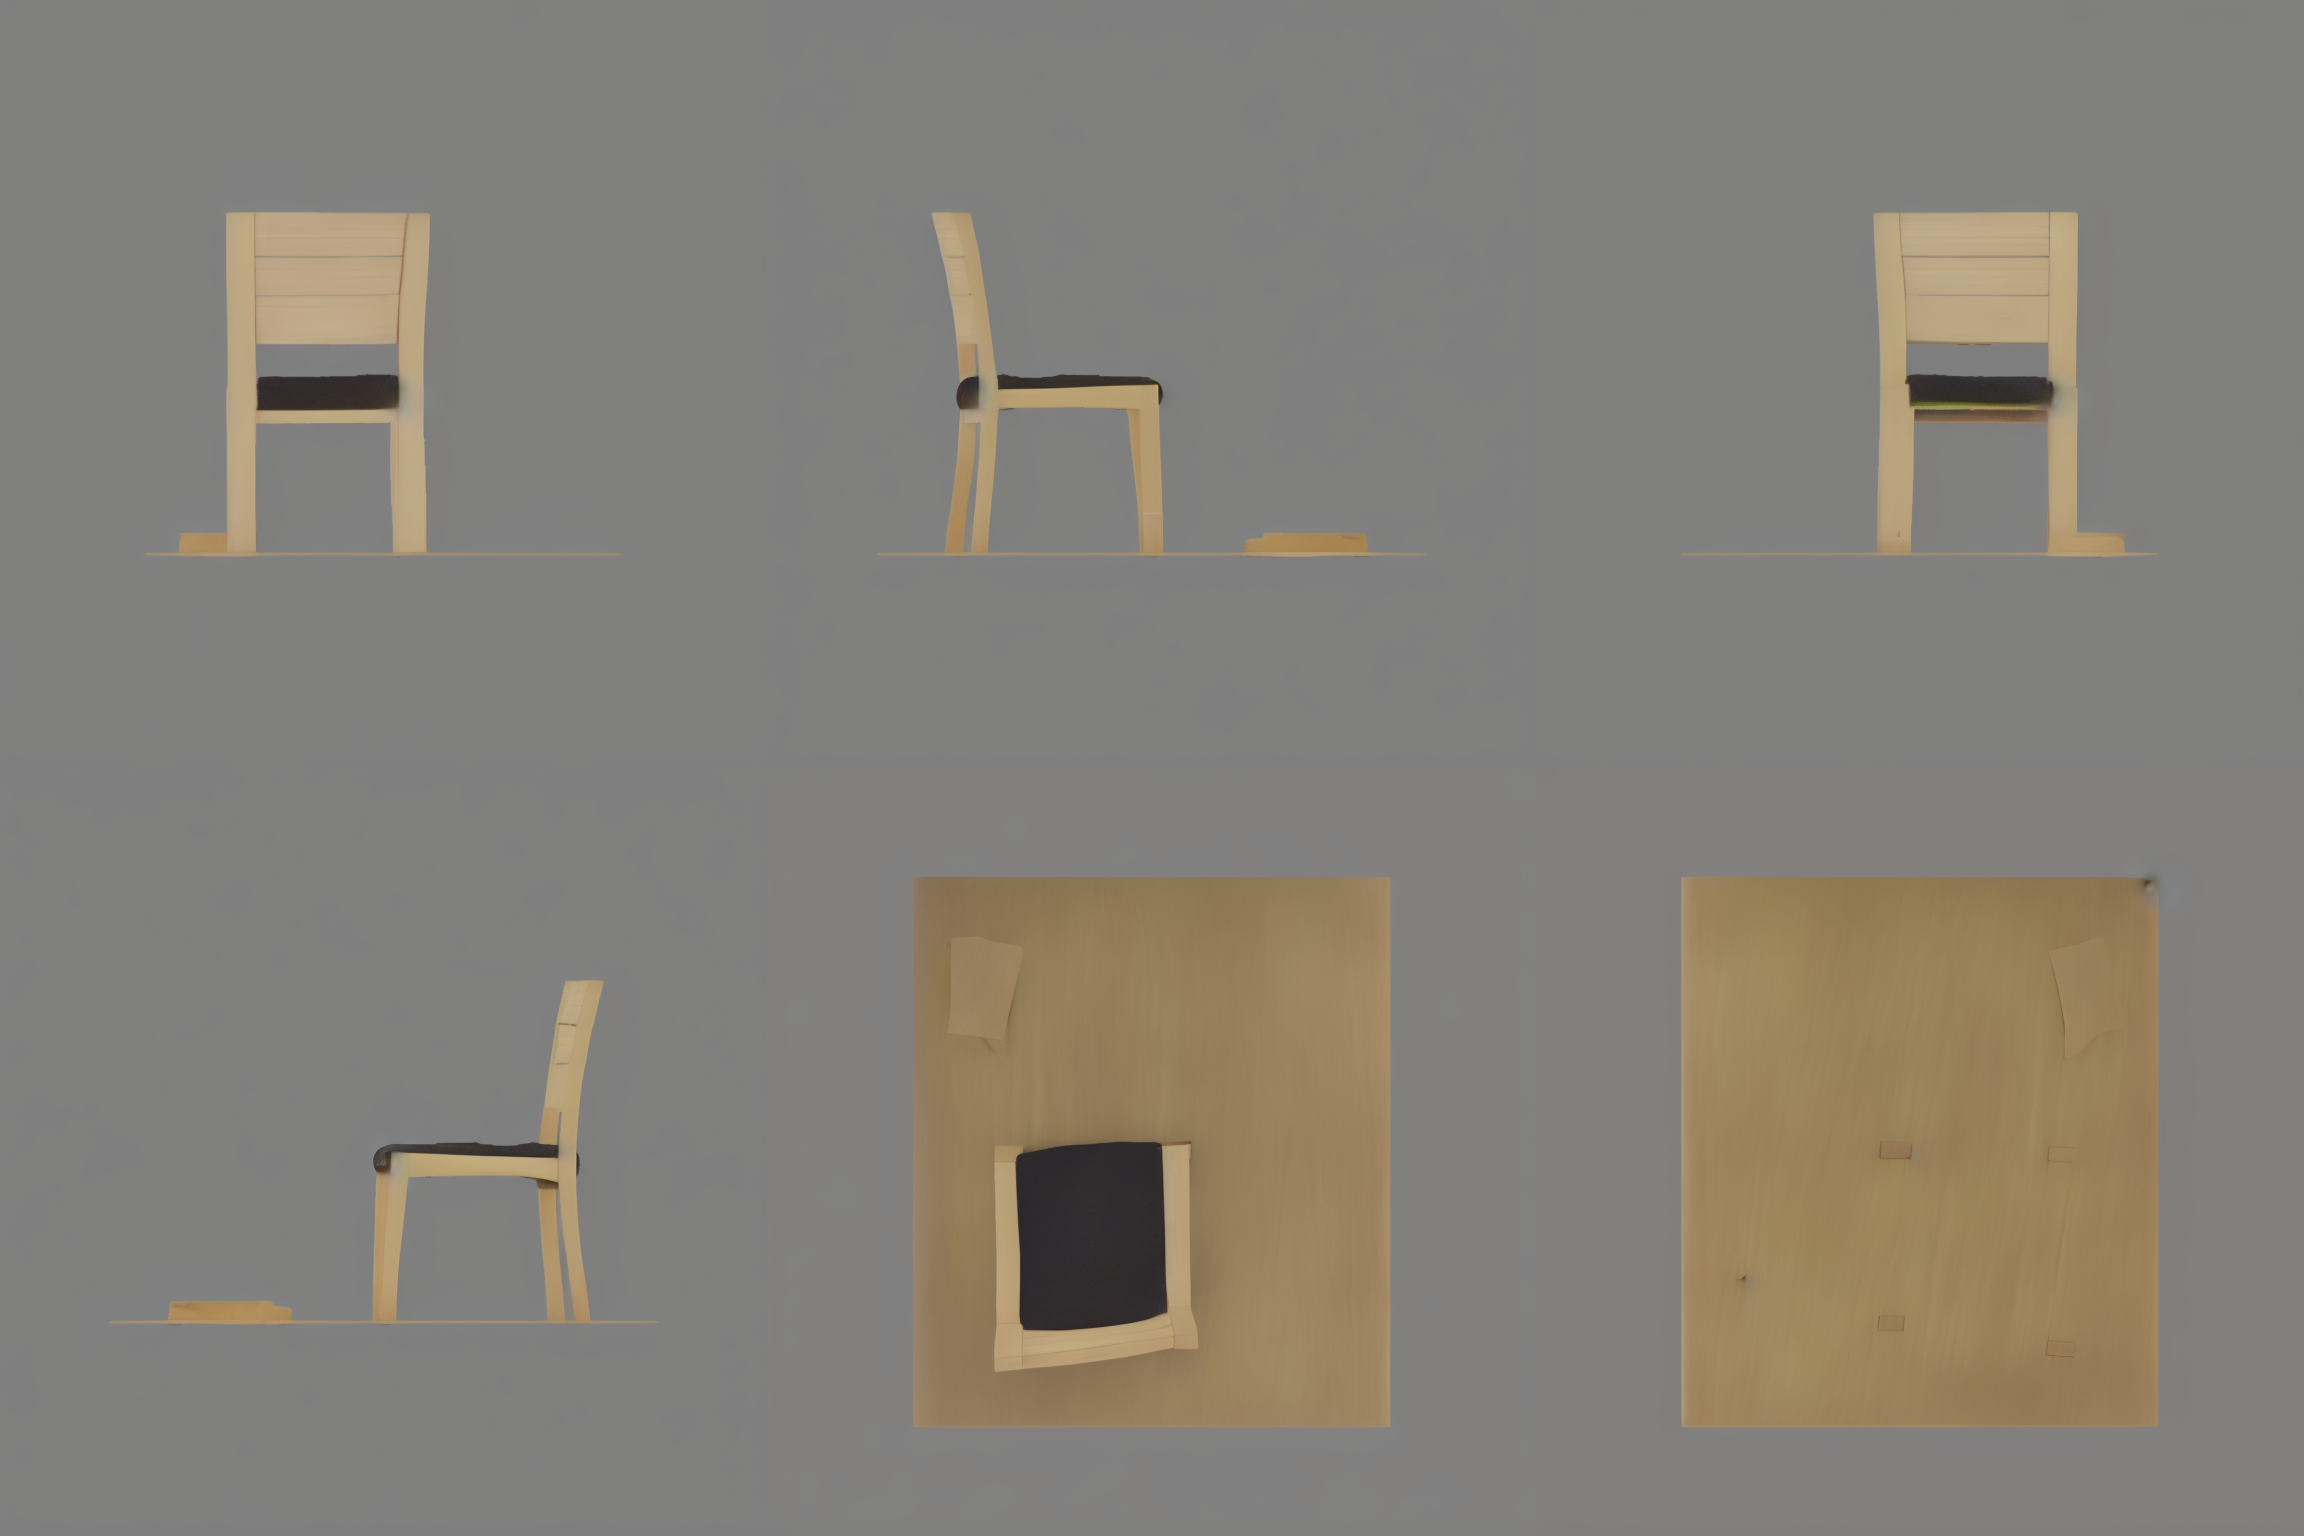
\includegraphics[width=\textwidth]{figures/chair_turnaround_sheet.png}
  \caption{%
    \textbf{TRELLIS.2 object reconstruction — chair turnaround sheet.}
    Multi-view orbit render of the textured GLB mesh produced by the
    \texttt{hull\_e2e} workflow: per-object SAM3 PLY crop $\to$ FLUX.2-dev
    view-inpainting $\to$ TRELLIS.2-4B mesh $\to$ PBR-baked GLB $\to$ FBX
    (Nanite game asset).
    The chair is rated \emph{good}; vacuum and toolbox likewise passed
    the object reconstruction gate (4/8 objects in this batch).
    Resolution: 2304$\times$1536.
  }
  \label{fig:objects}
\end{figure}

% ──────────────────────────────────────────────────────────────────────────────
% 7. CoMe-TSDF mesh in UE (baseline mesh deliverable)
% ──────────────────────────────────────────────────────────────────────────────
\begin{figure}[htbp]
  \centering
  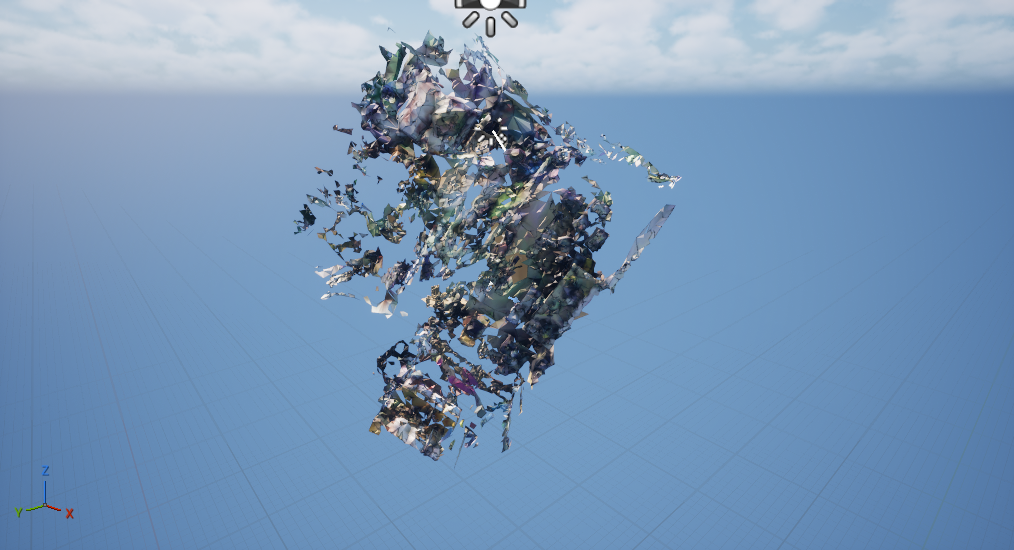
\includegraphics[width=\textwidth]{figures/ue_come_final.png}
  \caption{%
    \textbf{CoMe-TSDF room mesh game asset in UE\,5.8 (baseline mesh deliverable).}
    The scene-mesh branch: CoMe legacy \texttt{ScalableTSDFVolume} extraction,
    \texttt{mesh\_cleaner} (smooth=0, edge-length + connected-component cleanup),
    xatlas bake (\texttt{bake\_from\_vertex\_colors}), \texttt{blender\_obj\_to\_fbx},
    imported as a Nanite mesh.
    Characteristic TSDF blockiness on flat walls is visible; this image
    motivates the re-spine to NanoGS as the default room representation for
    blur-limited captures.
    Resolution: 1014$\times$550.
  }
  \label{fig:ue_come}
\end{figure}

% ──────────────────────────────────────────────────────────────────────────────
% 8. NanoGS splat render (1920×1080 B-view)
% ──────────────────────────────────────────────────────────────────────────────
\begin{figure}[htbp]
  \centering
  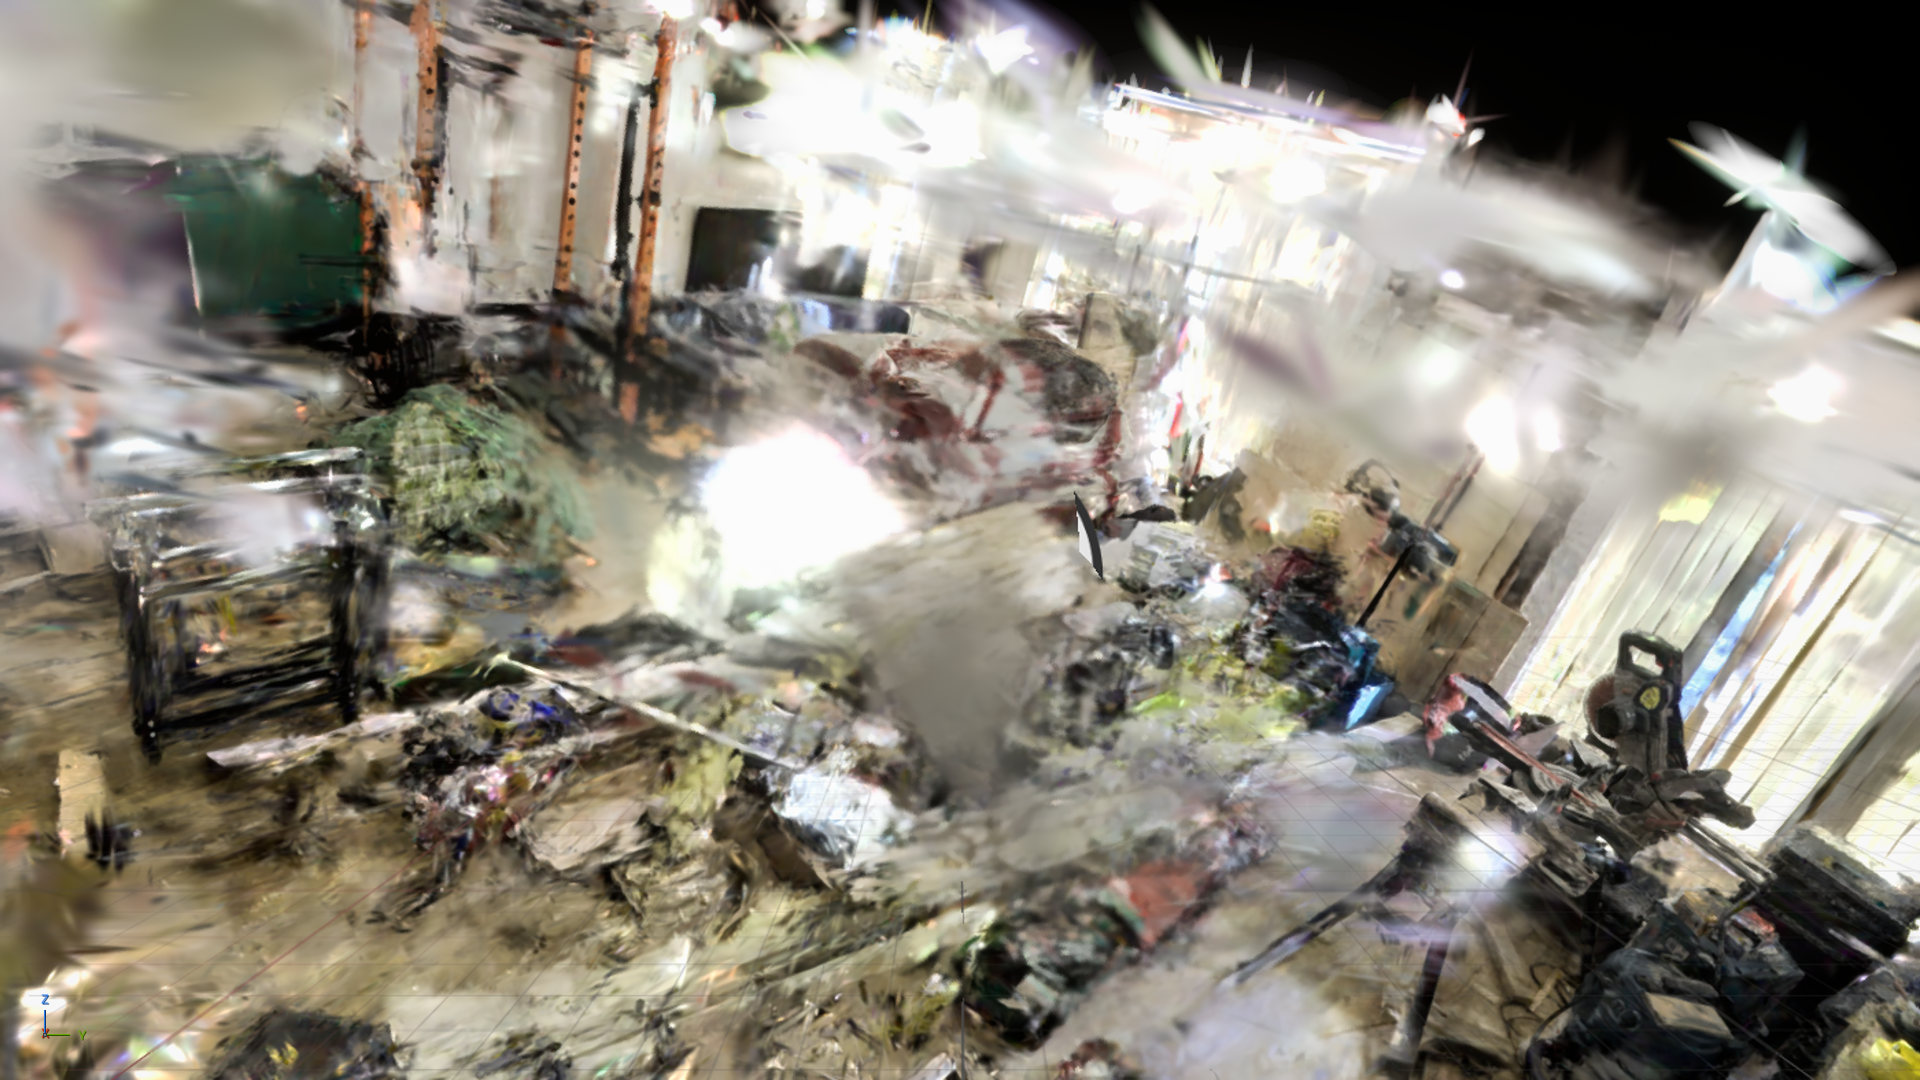
\includegraphics[width=\textwidth]{figures/ue_nanogs_room_B.png}
  \caption{%
    \textbf{NanoGS real-Gaussian splat in UE\,5.8 — interior view (B).}
    Second viewpoint of the NanoGS splat room, demonstrating depth and
    parallax of real Gaussian rendering at 1920$\times$1080.
    Comparison with Figure~\ref{fig:ue_come} illustrates the quality
    improvement of splat-hero over TSDF mesh for a motion-blur-limited
    capture: the splat faithfully preserves captured radiance;
    the mesh introduces geometric artefacts irrelevant to the capture.
  }
  \label{fig:ue_nanogs}
\end{figure}

% ──────────────────────────────────────────────────────────────────────────────
% 9. Hero perspective render (room + placed objects)
% ──────────────────────────────────────────────────────────────────────────────
\begin{figure}[htbp]
  \centering
  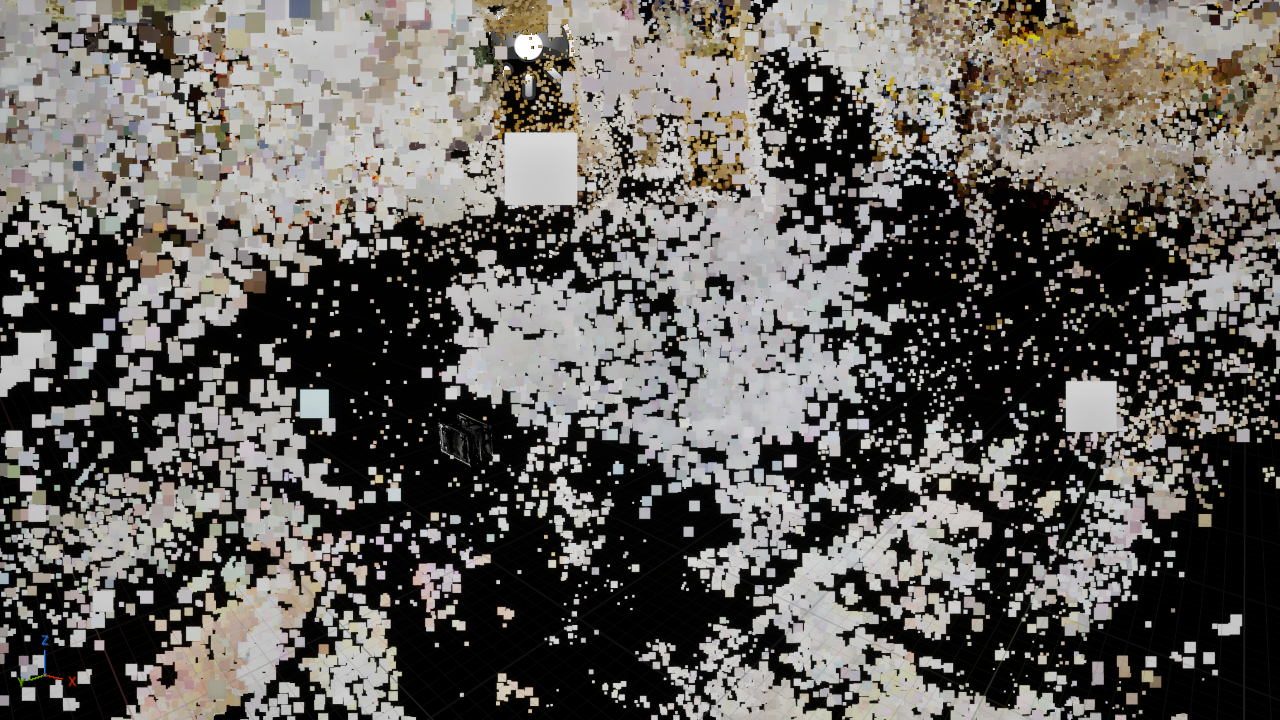
\includegraphics[width=\textwidth]{figures/ue_final_hero.png}
  \caption{%
    \textbf{Hero perspective render — dreamlab room with placed object FBXs.}
    A cinematic view of the assembled UE\,5.8 scene from the validated
    end-to-end run (2026-06-22): TSDF-mesh room (CoMe, pre-NanoGS re-spine)
    with TRELLIS.2 object FBXs placed by \texttt{ue\_place\_prescaled}.
    Resolution: 1280$\times$720.
    Serves as the primary before/after reference for evaluating the
    NanoGS re-spine (Figure~\ref{fig:nanogs_room}).
  }
  \label{fig:ue_hero}
\end{figure}

% ──────────────────────────────────────────────────────────────────────────────
% 10. Overhead dollhouse view
% ──────────────────────────────────────────────────────────────────────────────
\begin{figure}[htbp]
  \centering
  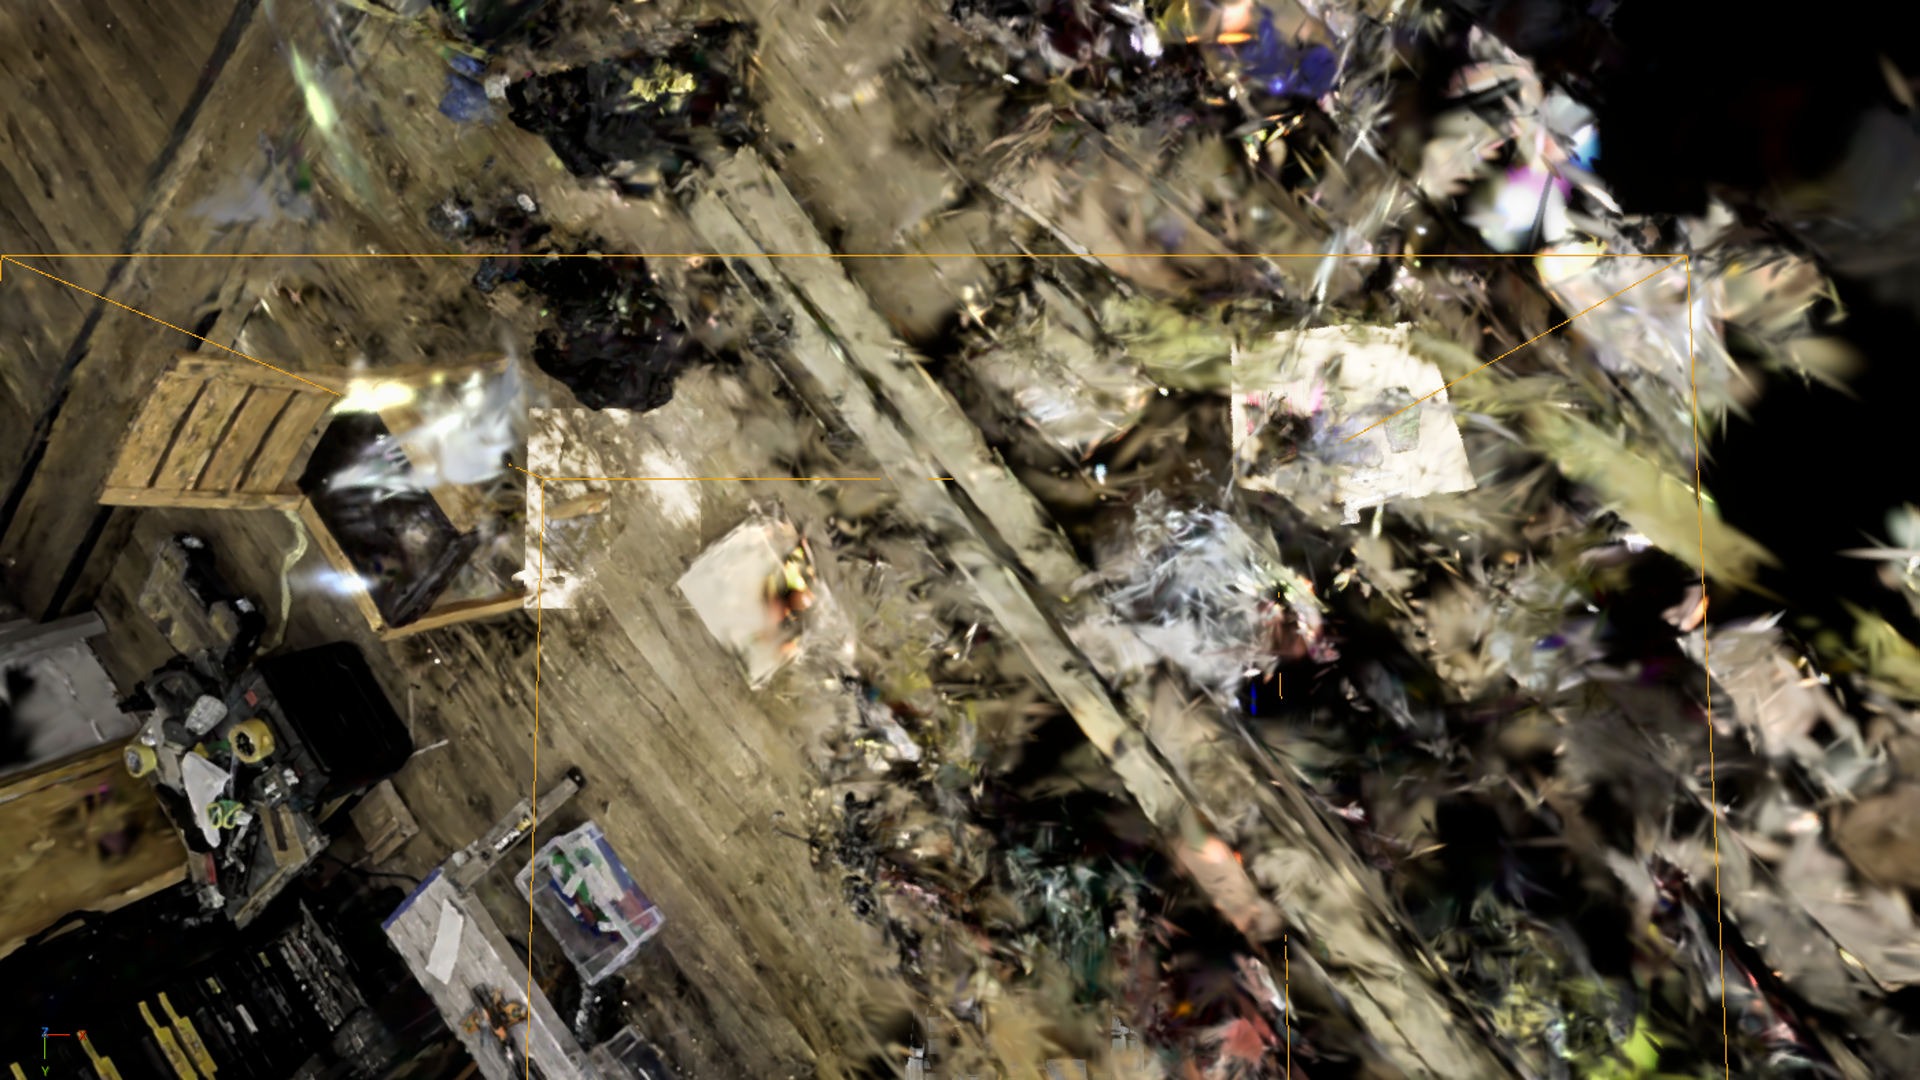
\includegraphics[width=\textwidth]{figures/ue_integrated_dollhouse.png}
  \caption{%
    \textbf{Overhead dollhouse view — integrated UE\,5.8 scene layout.}
    Top-down perspective revealing object placement, room geometry, and
    spatial relationships of the dreamlab scene.
    The dollhouse view is the standard QA checkpoint for scale fidelity
    and object-in-room alignment after \texttt{ue\_place\_prescaled}
    prescaling.
    Resolution: 1920$\times$1080.
  }
  \label{fig:ue_dollhouse}
\end{figure}

% Assumes \graphicspath{{figures/}} is set in the preamble (relative to report/v5/).
%
% Labels (for \ref / \autoref):
%   fig:router           — capture-adaptive router flowchart
%   fig:component_menu   — component-menu status flowchart
%   fig:architecture     — system architecture (container topology)
%   fig:nanogs_room      — NanoGS real-Gaussian splat render (canonical room hero)
%   fig:scene_integrated — fully integrated UE 5.8 scene (room + objects)
%   fig:objects          — TRELLIS.2 object turnaround sheet (chair)
%   fig:ue_come          — CoMe-TSDF mesh game asset in UE (baseline mesh)
%   fig:ue_nanogs        — NanoGS splat render (dreamlab room, 1920x1080)
%   fig:ue_hero          — Hero perspective render (room + placed objects)
%   fig:ue_dollhouse     — Overhead dollhouse view of integrated UE scene

% ──────────────────────────────────────────────────────────────────────────────
% 1. Capture-adaptive router
% ──────────────────────────────────────────────────────────────────────────────
\begin{figure}[htbp]
  \centering
  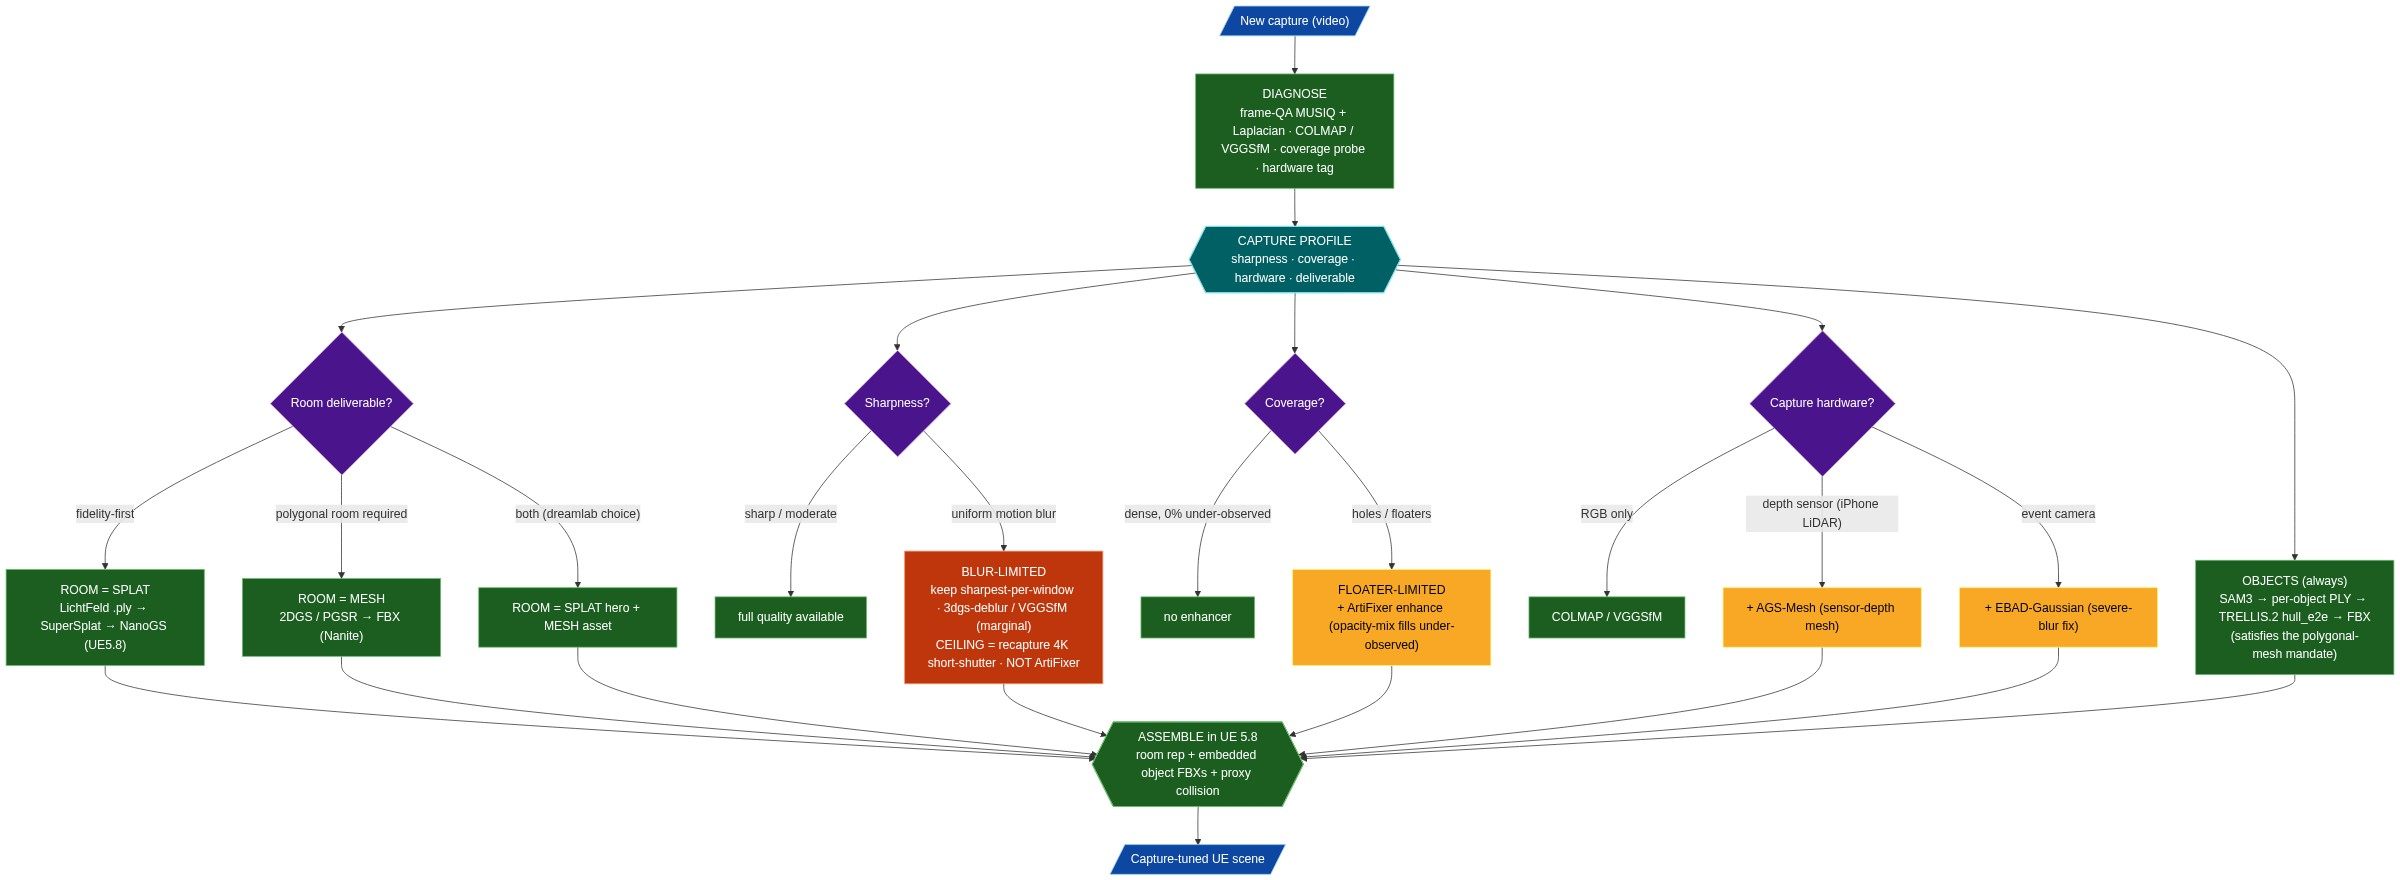
\includegraphics[width=\textwidth]{figures/router.jpg}
  \caption{%
    \textbf{Capture-adaptive router.}
    The pipeline diagnoses each new capture on four axes
    (sharpness via MUSIQ + full-resolution Laplacian, coverage via occupancy probe,
    available hardware, and deliverable type) and selects the configuration that
    fits the bottleneck.
    Green nodes are validated keepers; orange nodes are
    capture-conditional options; red nodes are blur-limited warnings.
    The dreamlab capture routes to Opt\,4 (splat hero + mesh asset + TRELLIS.2 objects)
    with a recapture flag as the quality ceiling.
  }
  \label{fig:router}
\end{figure}

% ──────────────────────────────────────────────────────────────────────────────
% 2. Component-menu flowchart
% ──────────────────────────────────────────────────────────────────────────────
\begin{figure}[htbp]
  \centering
  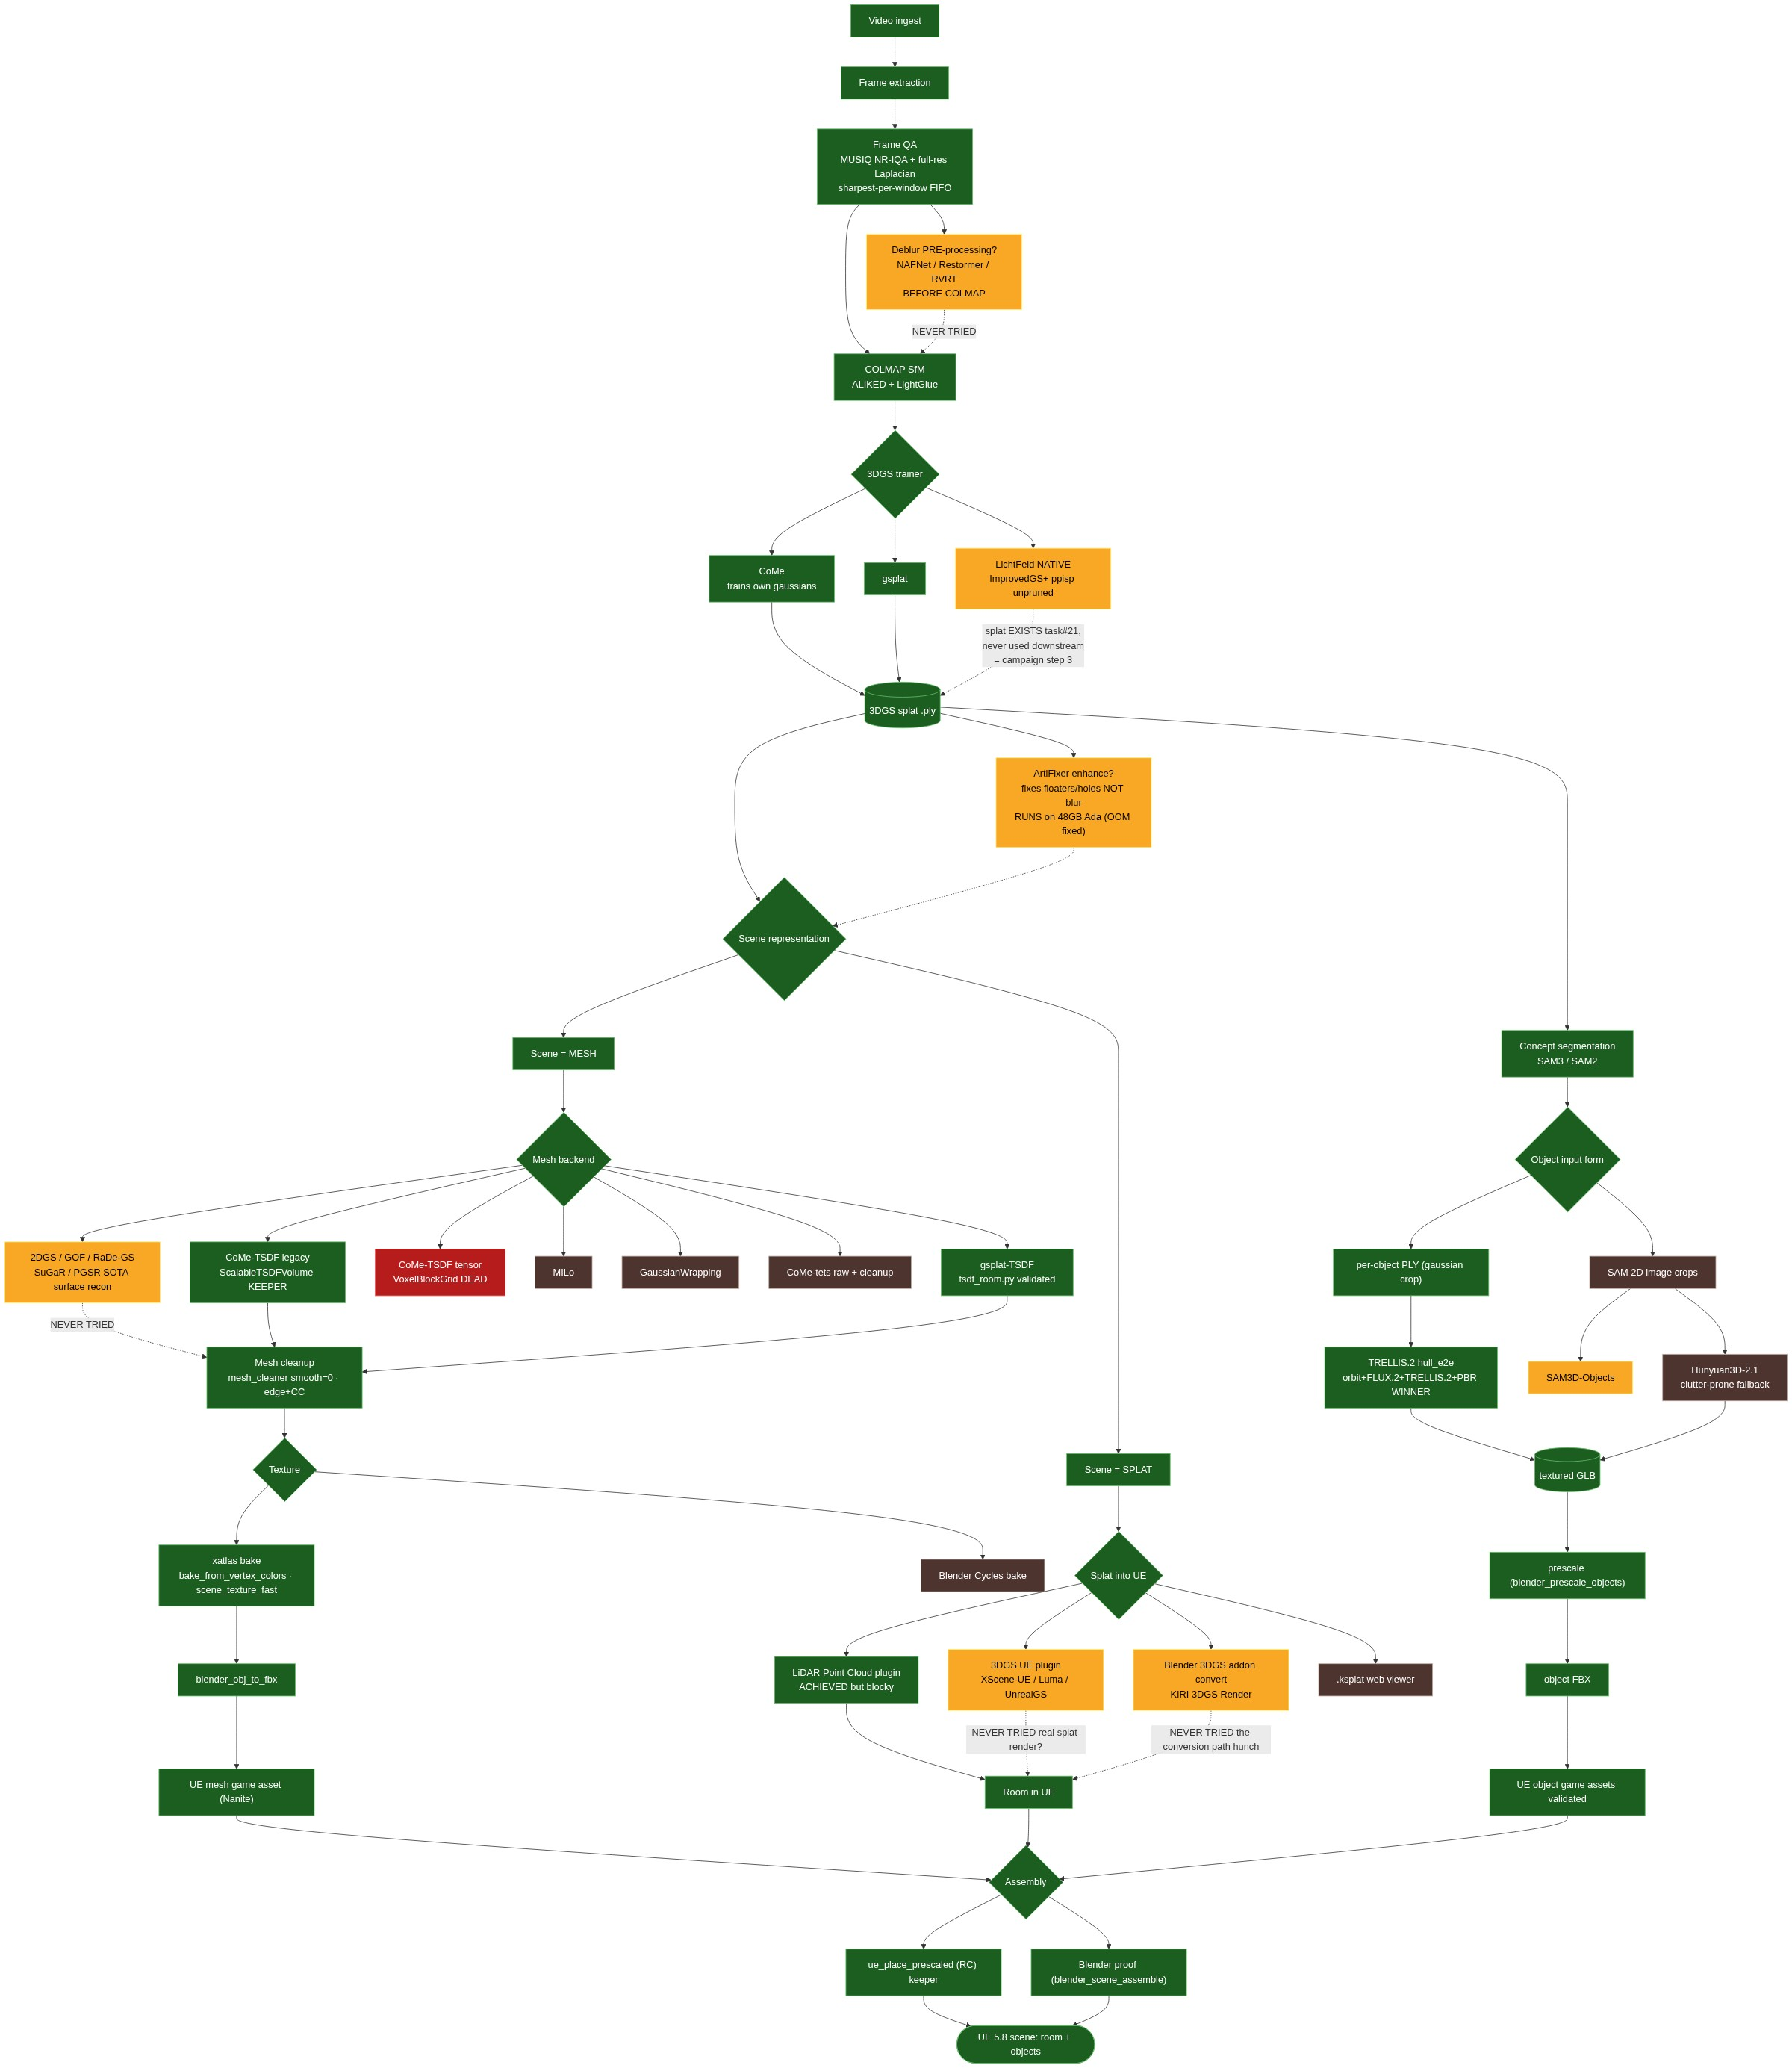
\includegraphics[width=\textwidth]{figures/component_menu.jpg}
  \caption{%
    \textbf{Full component-menu status chart (validated 2026-06-25).}
    Every branch of the Vitrine toolkit from video ingest to UE\,5.8 delivery.
    Colour coding: \emph{green} = validated keeper in active use;
    \emph{brown} = exercised but subordinate / fallback;
    \emph{red} = tried and abandoned;
    \emph{yellow} = plausible, never run.
    The chart is the canonical record of what has and has not been exercised;
    dashed arrows mark paths that remain open research items
    (SAM3D-Objects, BAD-Gaussians deblur, PGSR/2DGS surface reconstruction).
  }
  \label{fig:component_menu}
\end{figure}

% ──────────────────────────────────────────────────────────────────────────────
% 3. System architecture (container topology)
% ──────────────────────────────────────────────────────────────────────────────
\begin{figure}[htbp]
  \centering
  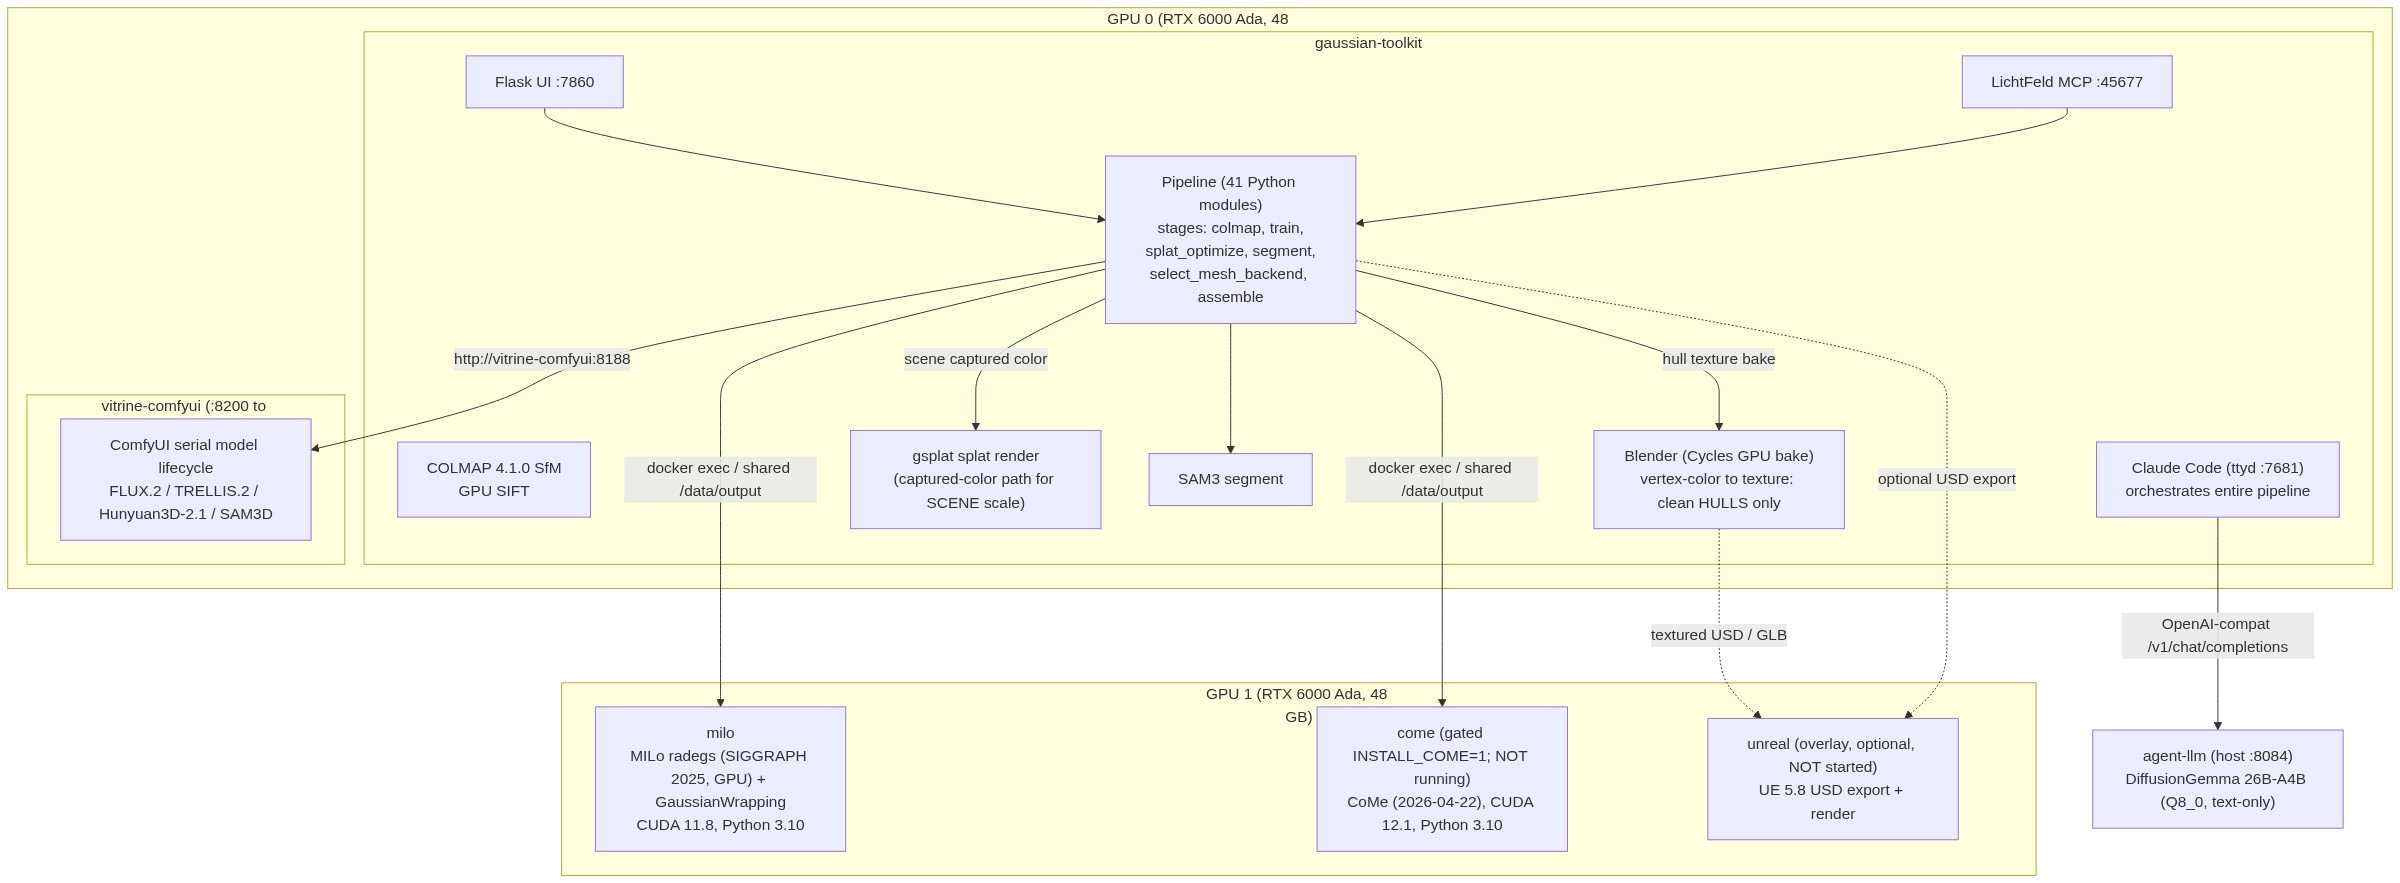
\includegraphics[width=\textwidth]{figures/architecture.jpg}
  \caption{%
    \textbf{Vitrine system architecture — Docker container topology.}
    Two RTX\,6000\,Ada GPUs (48\,GB each) host the six-container stack.
    GPU\,0 runs the \texttt{gaussian-toolkit} orchestrator (COLMAP, LichtFeld
    3DGS, SAM3, Flask\,UI, LichtFeld\,MCP on port\,45677) and
    \texttt{vitrine-comfyui} (FLUX.2\,/\,TRELLIS.2\,/\,Hunyuan3D-2.1, serial
    model lifecycle).
    GPU\,1 hosts the \texttt{milo} sidecar (MILo radegs, CUDA\,11.8) and the
    optional \texttt{come} (CoMe, CUDA\,12.1) and \texttt{unreal} (UE\,5.8)
    overlay containers.
    DiffusionGemma\,26B-A4B runs on the host at port\,8084 as the local text
    reasoner.
    All pipeline containers share \texttt{v2g-net}; the agentbox (Claude Code)
    reaches them via the shared \texttt{visionclaw\_network}.
  }
  \label{fig:architecture}
\end{figure}

% ──────────────────────────────────────────────────────────────────────────────
% 4. NanoGS room splat (docs canonical hero)
% ──────────────────────────────────────────────────────────────────────────────
\begin{figure}[htbp]
  \centering
  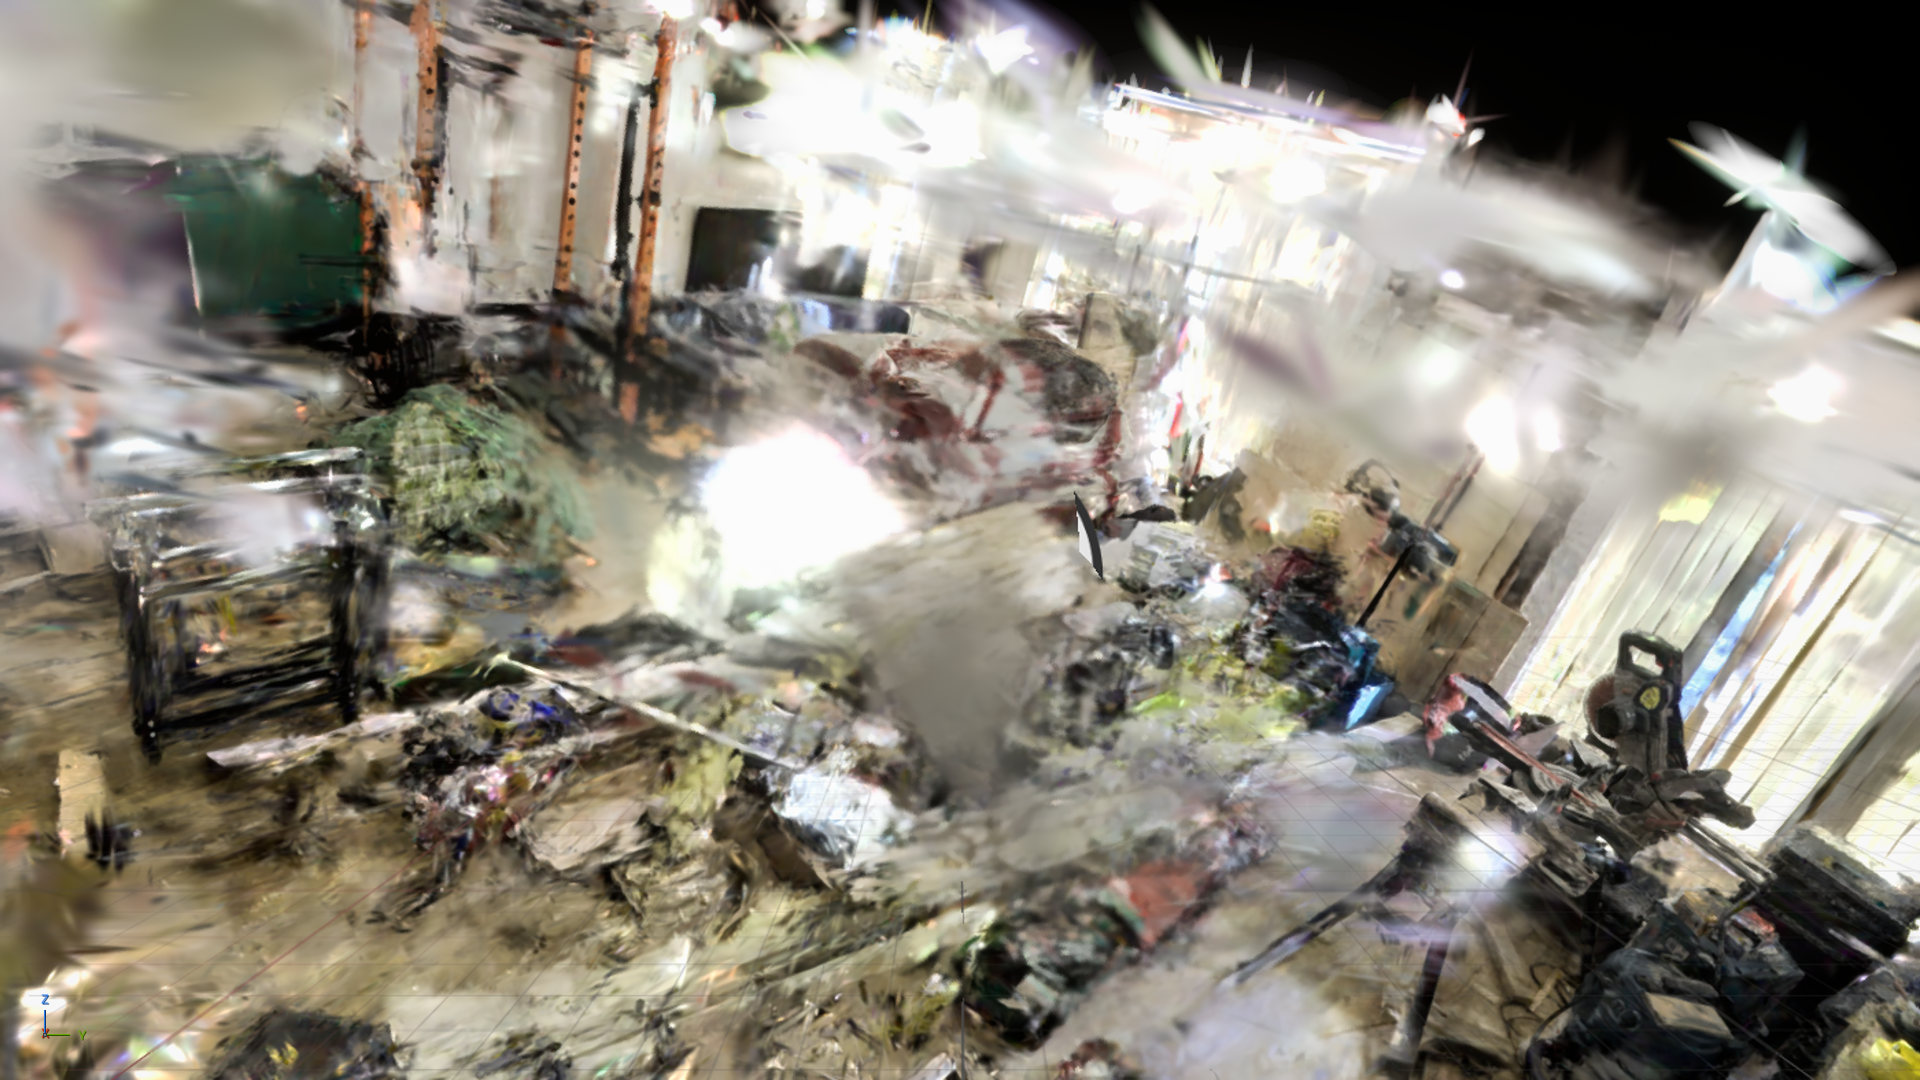
\includegraphics[width=\textwidth]{figures/nanogs_room_splat.png}
  \caption{%
    \textbf{Dreamlab room — NanoGS real-Gaussian splat render (canonical hero).}
    The LichtFeld-native \texttt{splat\_30000.ply}, cleaned via SuperSplat and
    loaded into the NanoGS\,(MIT) UE\,5.8 plugin, rendered at 1920$\times$1080.
    This replaces the earlier LiDAR point-cloud workaround and constitutes
    campaign step\,3: lean-on-LichtFeld native output for the room representation.
    Motion-blur softness in the source splat reflects the dreamlab capture
    constraint (MUSIQ $\approx$ 31); recapture at 4\,K\,/\,short shutter is the
    ceiling lever, not a pipeline limitation.
  }
  \label{fig:nanogs_room}
\end{figure}

% ──────────────────────────────────────────────────────────────────────────────
% 5. Fully integrated UE 5.8 scene
% ──────────────────────────────────────────────────────────────────────────────
\begin{figure}[htbp]
  \centering
  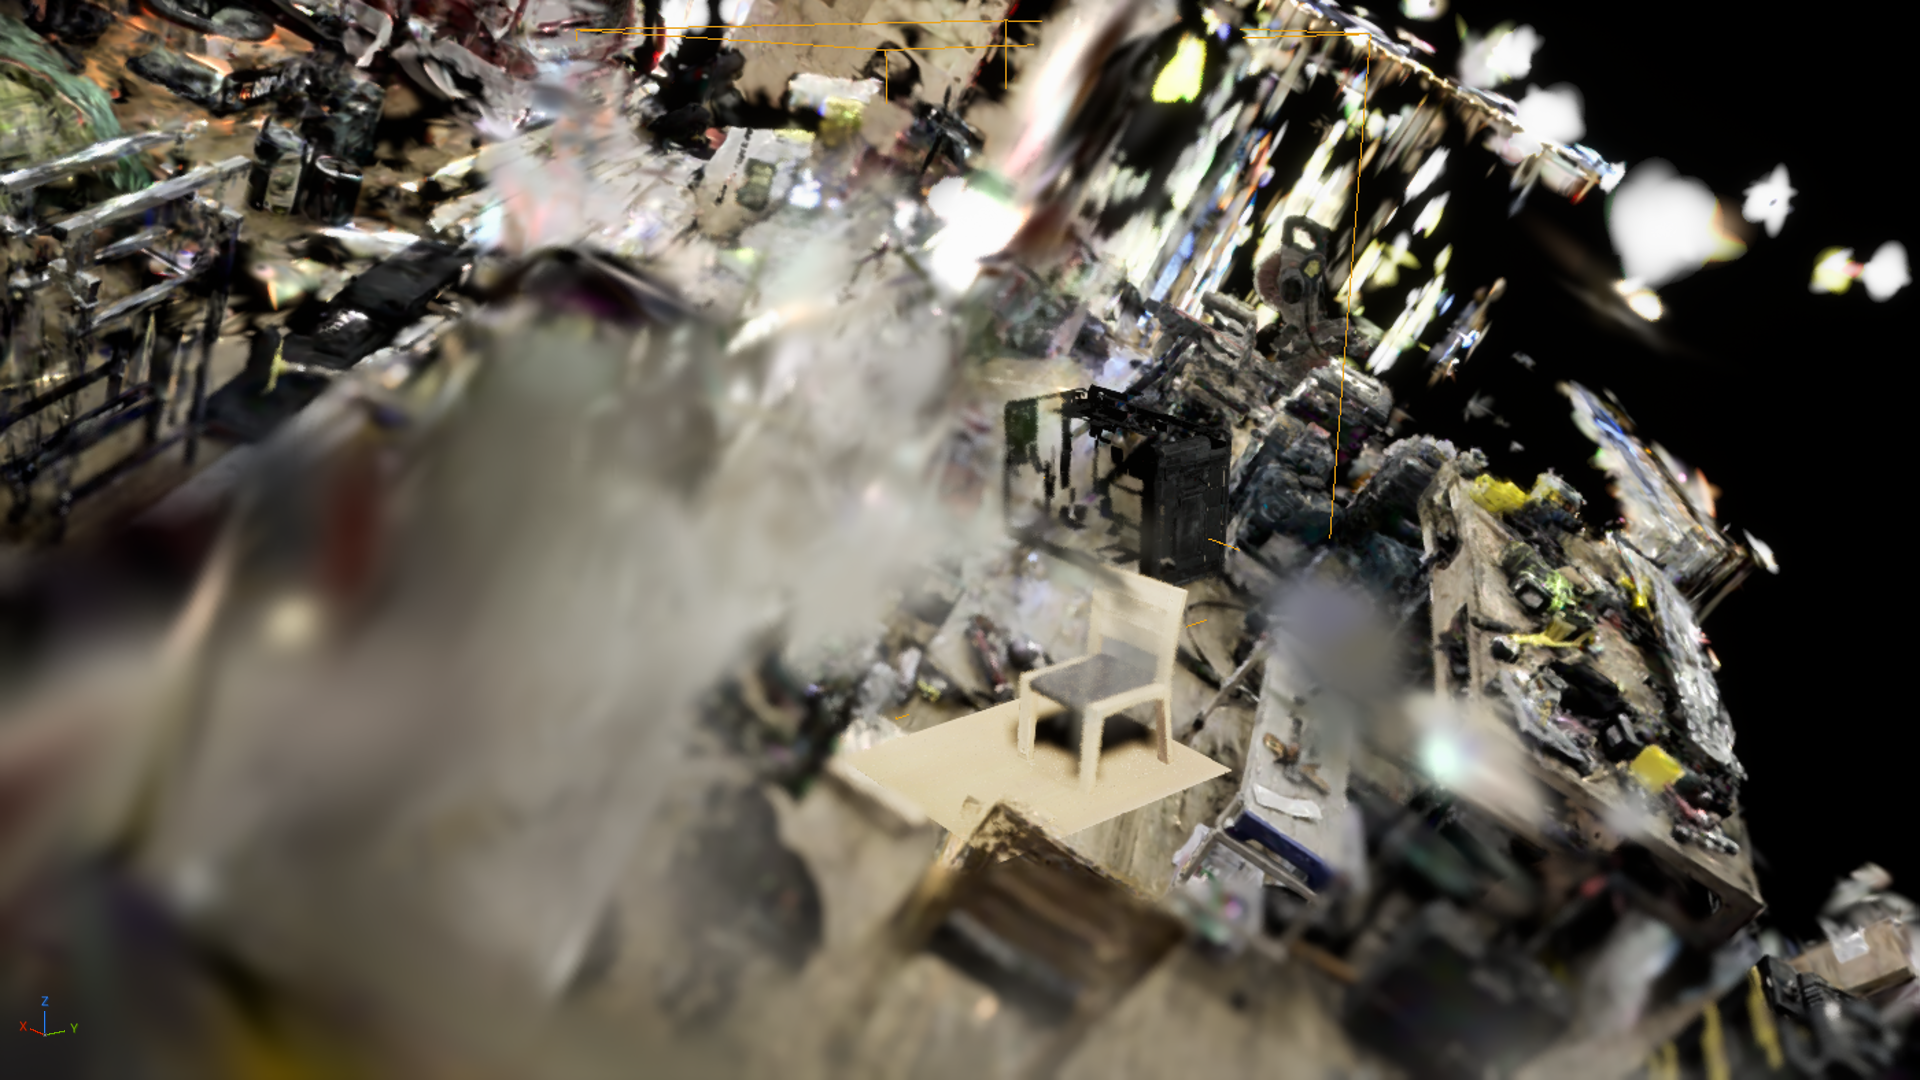
\includegraphics[width=\textwidth]{figures/scene_integrated.png}
  \caption{%
    \textbf{Integrated UE\,5.8 scene — room splat with placed TRELLIS.2 object FBXs.}
    The assembled deliverable: NanoGS splat room (hero representation) with
    chair, vacuum, and toolbox FBXs (TRELLIS.2 \texttt{hull\_e2e},
    prescaled via \texttt{blender\_prescale\_objects}) placed by
    \texttt{ue\_place\_prescaled}.
    Objects are Nanite game assets with baked PBR textures; the room splat
    renders real Gaussians.
    This image is the \emph{docs} canonical integrated-scene reference.
  }
  \label{fig:scene_integrated}
\end{figure}

% ──────────────────────────────────────────────────────────────────────────────
% 6. TRELLIS.2 object turnaround sheet (chair)
% ──────────────────────────────────────────────────────────────────────────────
\begin{figure}[htbp]
  \centering
  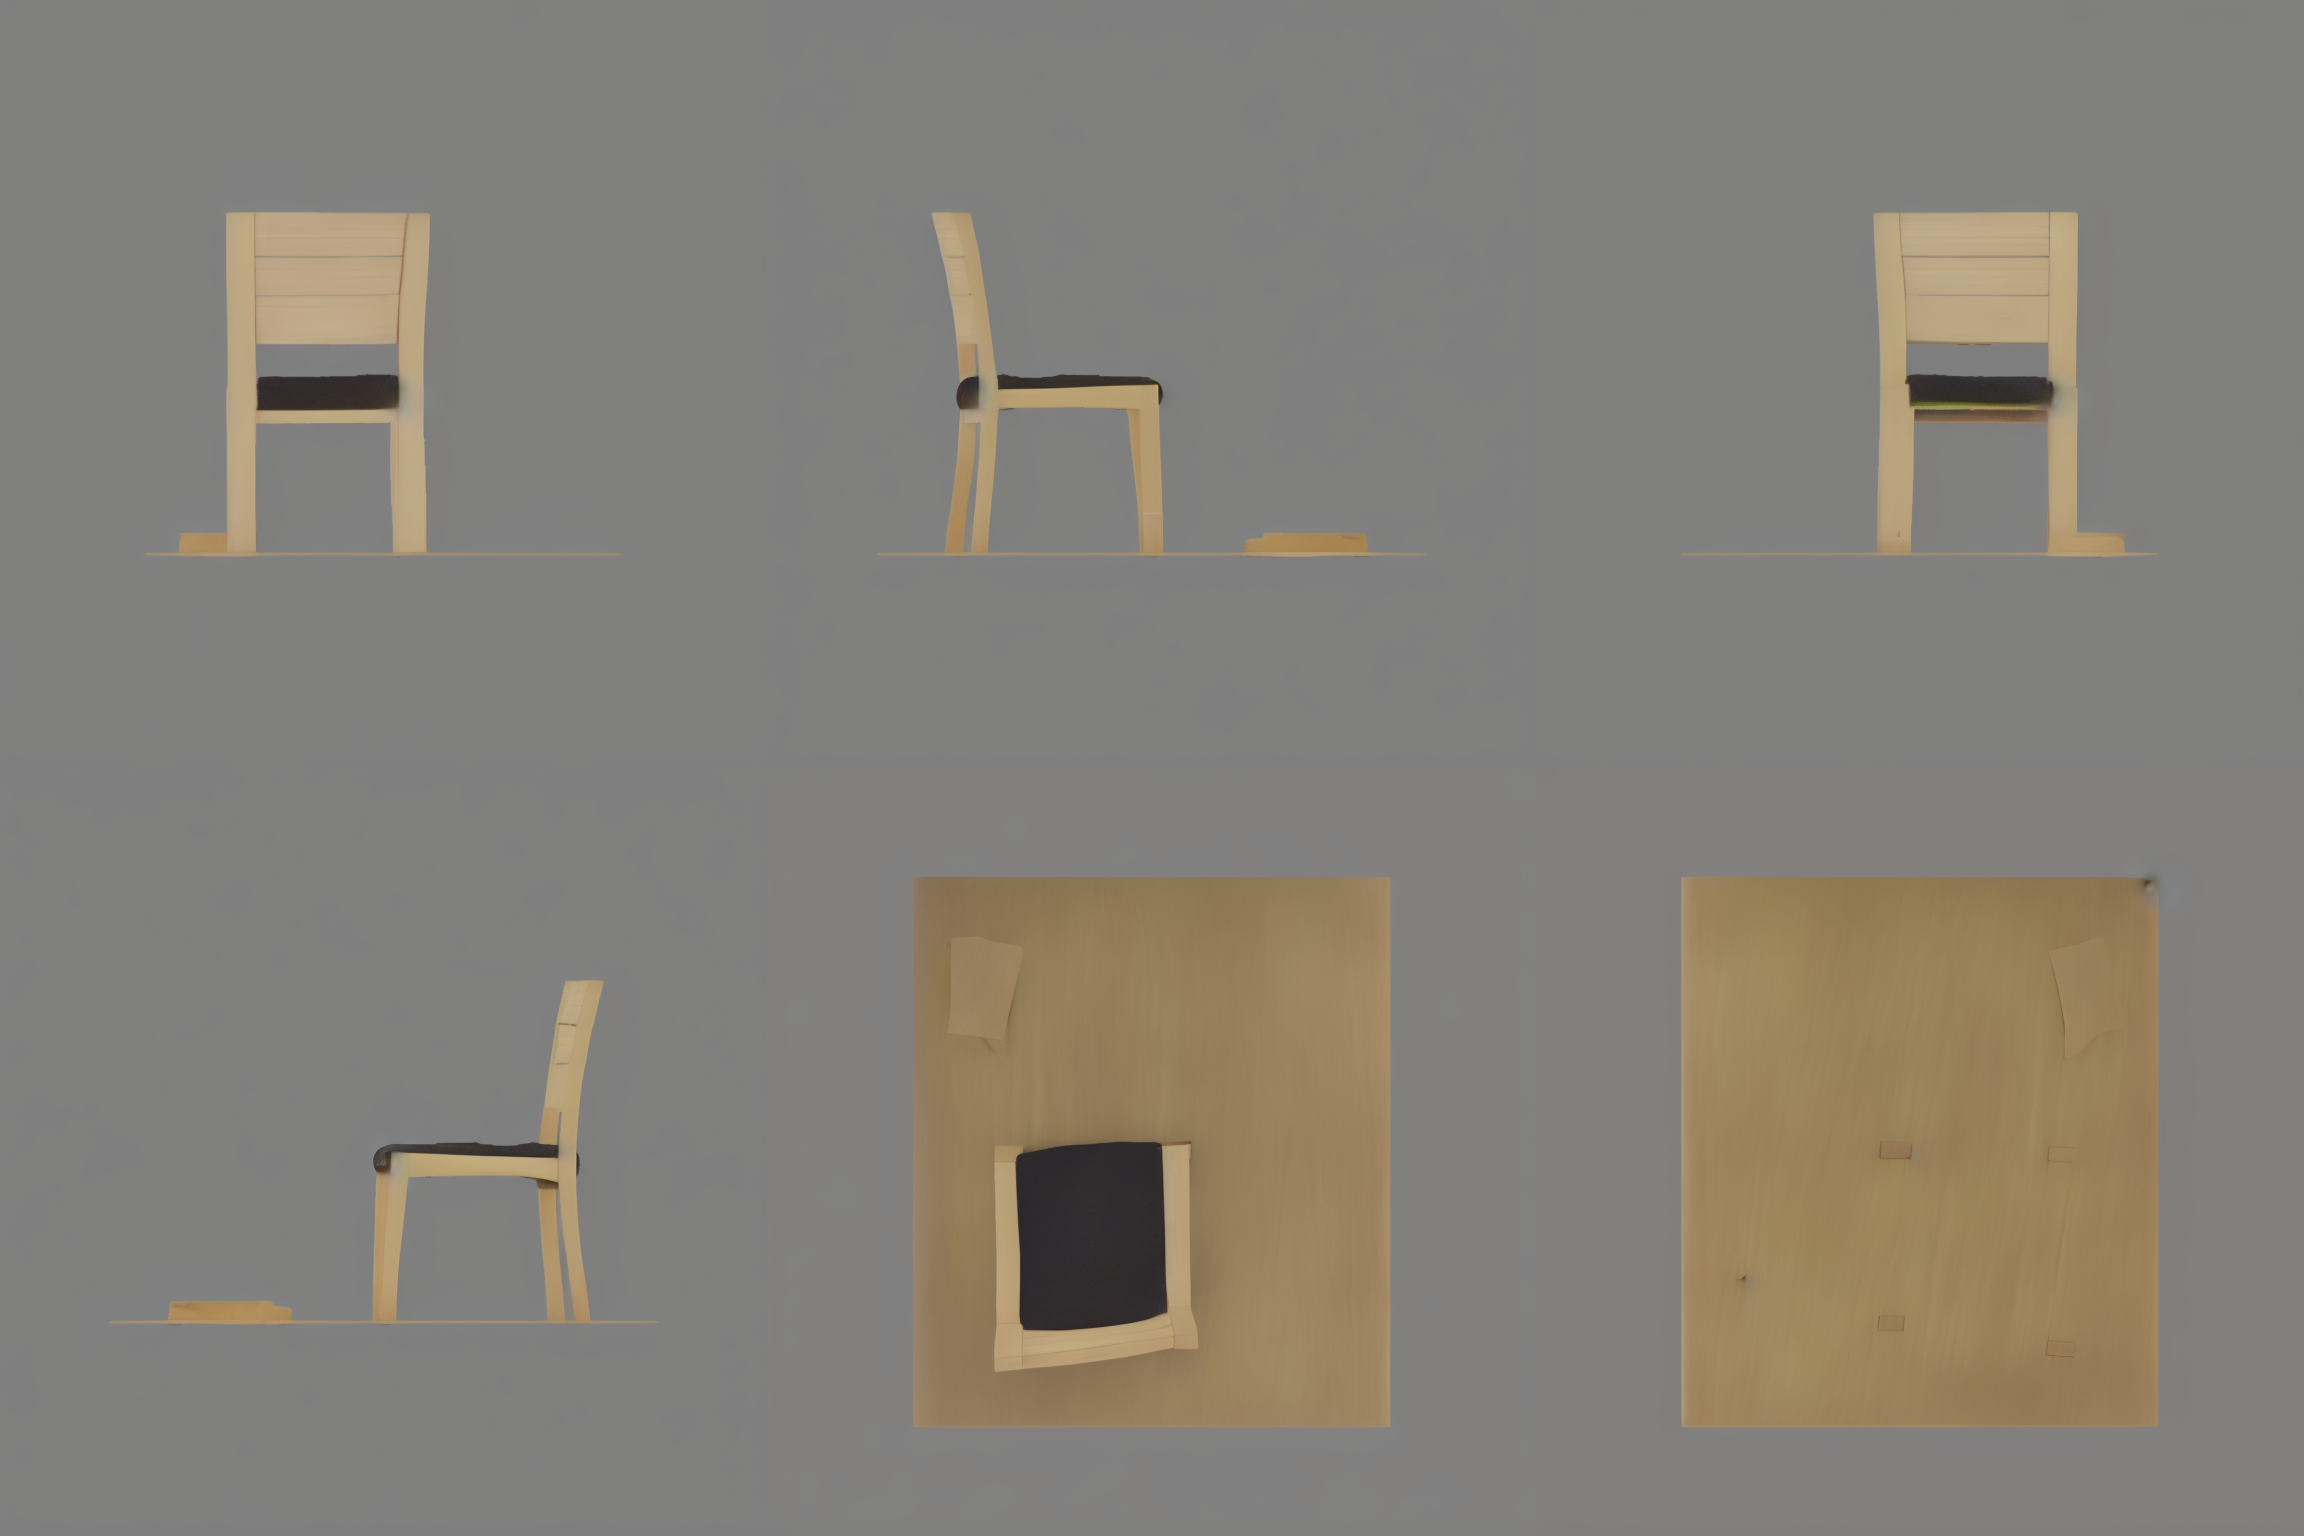
\includegraphics[width=\textwidth]{figures/chair_turnaround_sheet.png}
  \caption{%
    \textbf{TRELLIS.2 object reconstruction — chair turnaround sheet.}
    Multi-view orbit render of the textured GLB mesh produced by the
    \texttt{hull\_e2e} workflow: per-object SAM3 PLY crop $\to$ FLUX.2-dev
    view-inpainting $\to$ TRELLIS.2-4B mesh $\to$ PBR-baked GLB $\to$ FBX
    (Nanite game asset).
    The chair is rated \emph{good}; vacuum and toolbox likewise passed
    the object reconstruction gate (4/8 objects in this batch).
    Resolution: 2304$\times$1536.
  }
  \label{fig:objects}
\end{figure}

% ──────────────────────────────────────────────────────────────────────────────
% 7. CoMe-TSDF mesh in UE (baseline mesh deliverable)
% ──────────────────────────────────────────────────────────────────────────────
\begin{figure}[htbp]
  \centering
  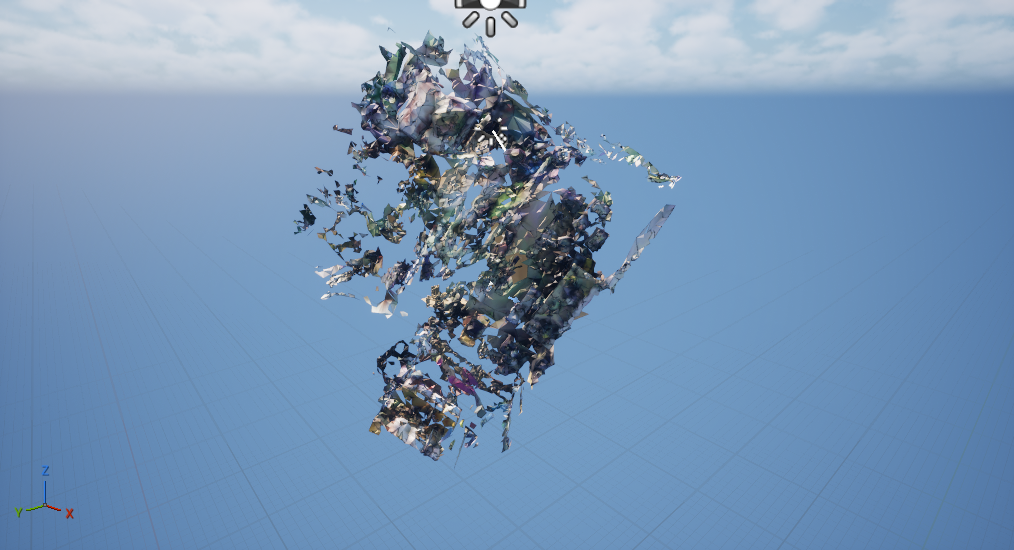
\includegraphics[width=\textwidth]{figures/ue_come_final.png}
  \caption{%
    \textbf{CoMe-TSDF room mesh game asset in UE\,5.8 (baseline mesh deliverable).}
    The scene-mesh branch: CoMe legacy \texttt{ScalableTSDFVolume} extraction,
    \texttt{mesh\_cleaner} (smooth=0, edge-length + connected-component cleanup),
    xatlas bake (\texttt{bake\_from\_vertex\_colors}), \texttt{blender\_obj\_to\_fbx},
    imported as a Nanite mesh.
    Characteristic TSDF blockiness on flat walls is visible; this image
    motivates the re-spine to NanoGS as the default room representation for
    blur-limited captures.
    Resolution: 1014$\times$550.
  }
  \label{fig:ue_come}
\end{figure}

% ──────────────────────────────────────────────────────────────────────────────
% 8. NanoGS splat render (1920×1080 B-view)
% ──────────────────────────────────────────────────────────────────────────────
\begin{figure}[htbp]
  \centering
  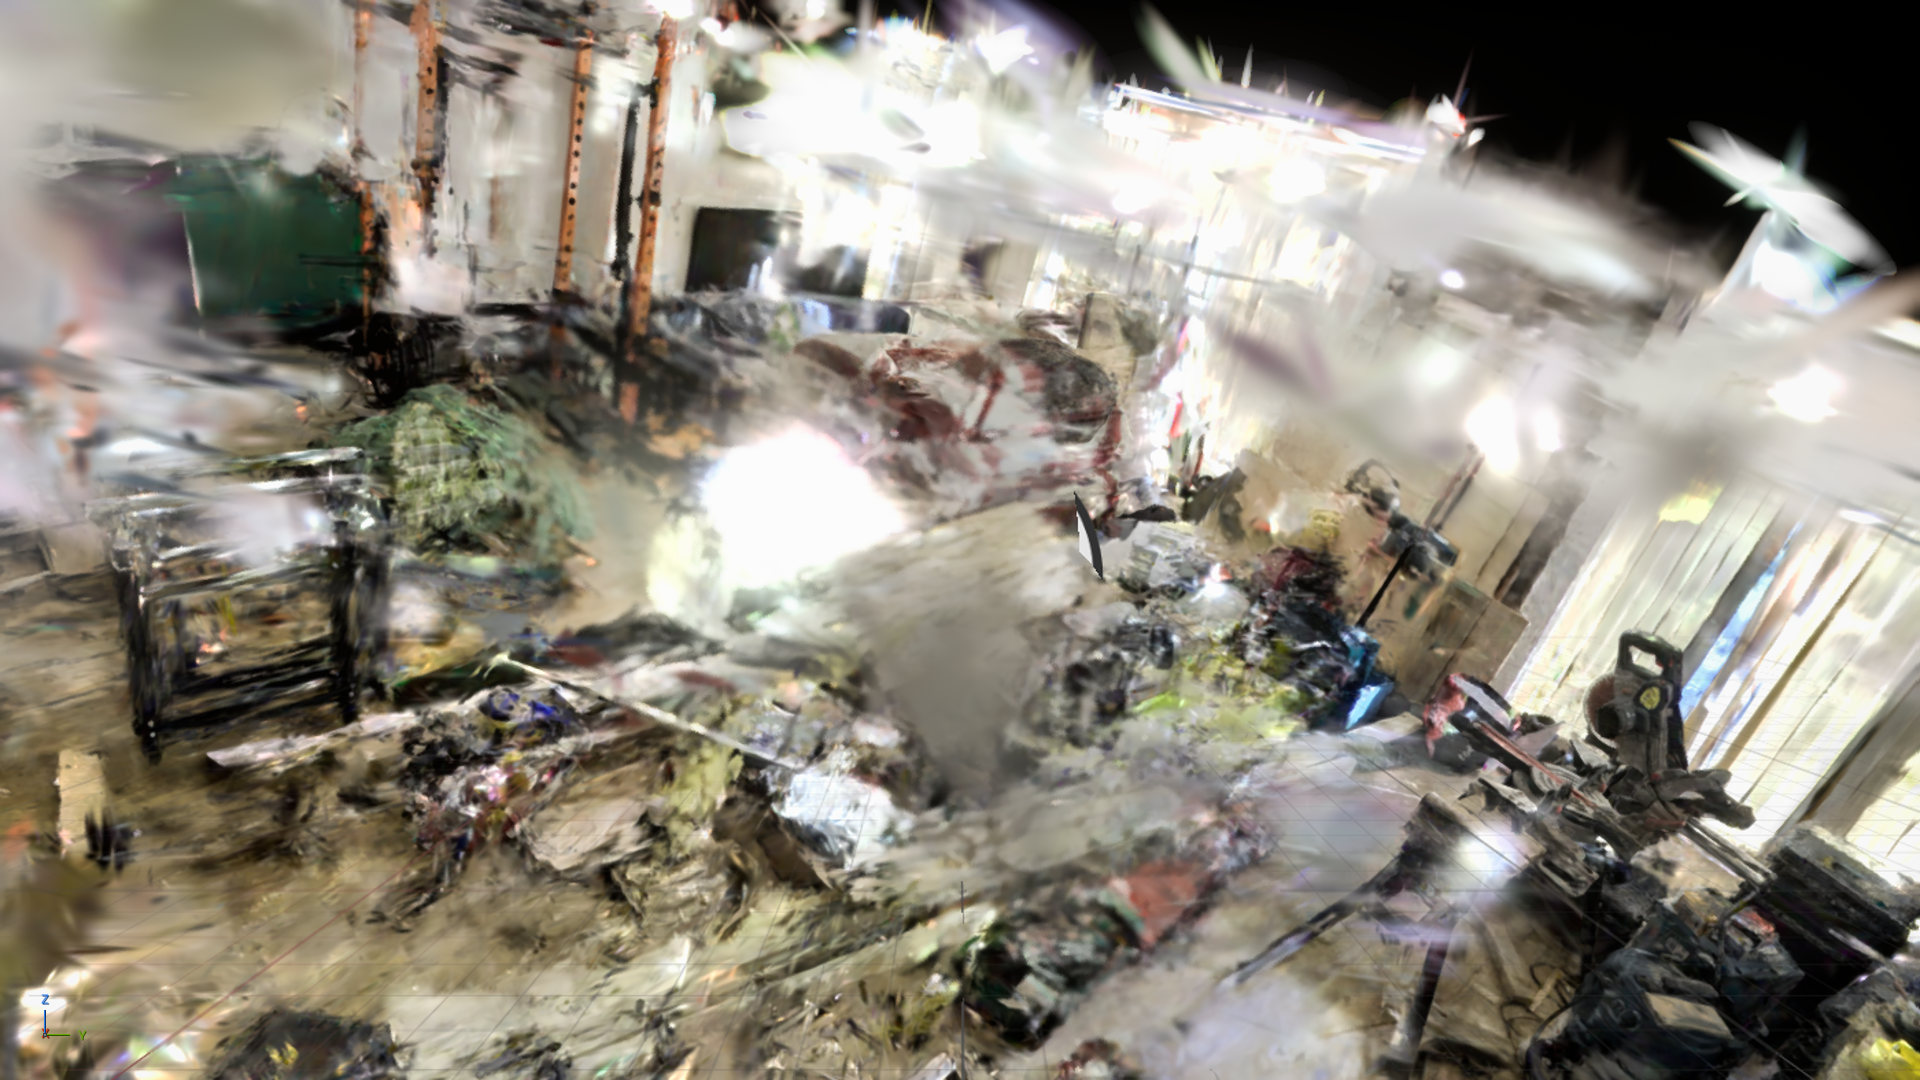
\includegraphics[width=\textwidth]{figures/ue_nanogs_room_B.png}
  \caption{%
    \textbf{NanoGS real-Gaussian splat in UE\,5.8 — interior view (B).}
    Second viewpoint of the NanoGS splat room, demonstrating depth and
    parallax of real Gaussian rendering at 1920$\times$1080.
    Comparison with Figure~\ref{fig:ue_come} illustrates the quality
    improvement of splat-hero over TSDF mesh for a motion-blur-limited
    capture: the splat faithfully preserves captured radiance;
    the mesh introduces geometric artefacts irrelevant to the capture.
  }
  \label{fig:ue_nanogs}
\end{figure}

% ──────────────────────────────────────────────────────────────────────────────
% 9. Hero perspective render (room + placed objects)
% ──────────────────────────────────────────────────────────────────────────────
\begin{figure}[htbp]
  \centering
  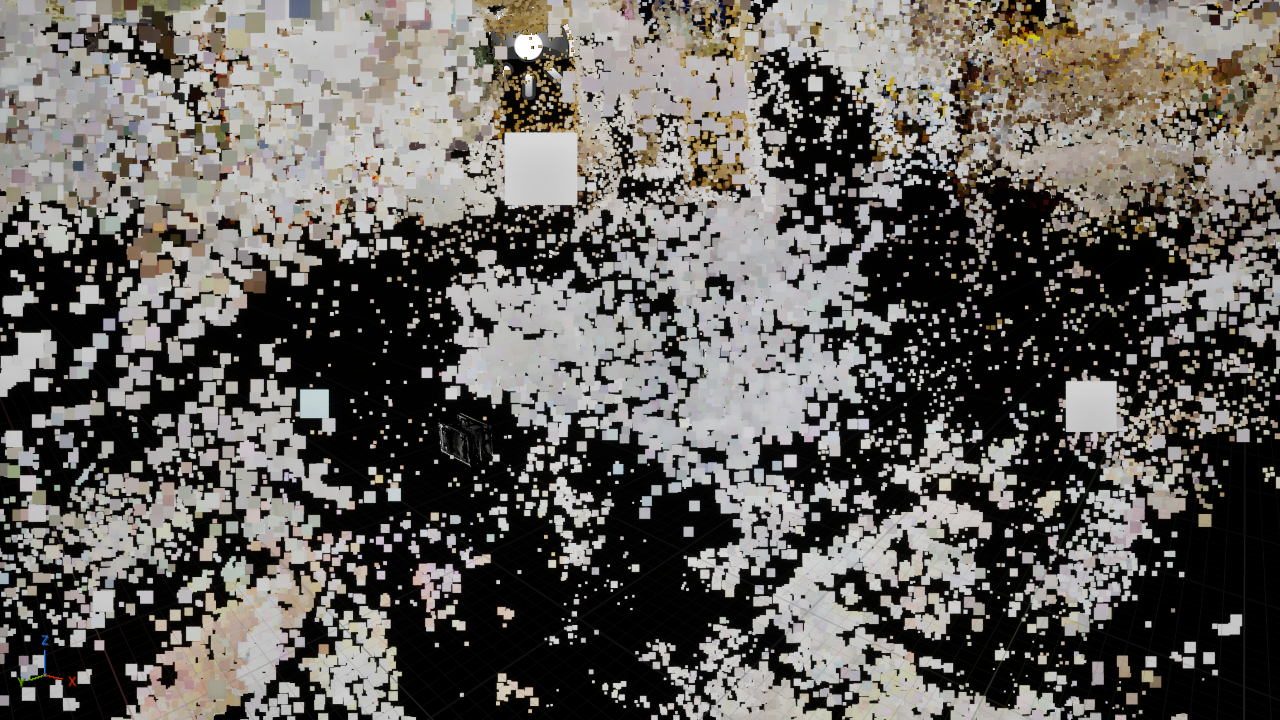
\includegraphics[width=\textwidth]{figures/ue_final_hero.png}
  \caption{%
    \textbf{Hero perspective render — dreamlab room with placed object FBXs.}
    A cinematic view of the assembled UE\,5.8 scene from the validated
    end-to-end run (2026-06-22): TSDF-mesh room (CoMe, pre-NanoGS re-spine)
    with TRELLIS.2 object FBXs placed by \texttt{ue\_place\_prescaled}.
    Resolution: 1280$\times$720.
    Serves as the primary before/after reference for evaluating the
    NanoGS re-spine (Figure~\ref{fig:nanogs_room}).
  }
  \label{fig:ue_hero}
\end{figure}

% ──────────────────────────────────────────────────────────────────────────────
% 10. Overhead dollhouse view
% ──────────────────────────────────────────────────────────────────────────────
\begin{figure}[htbp]
  \centering
  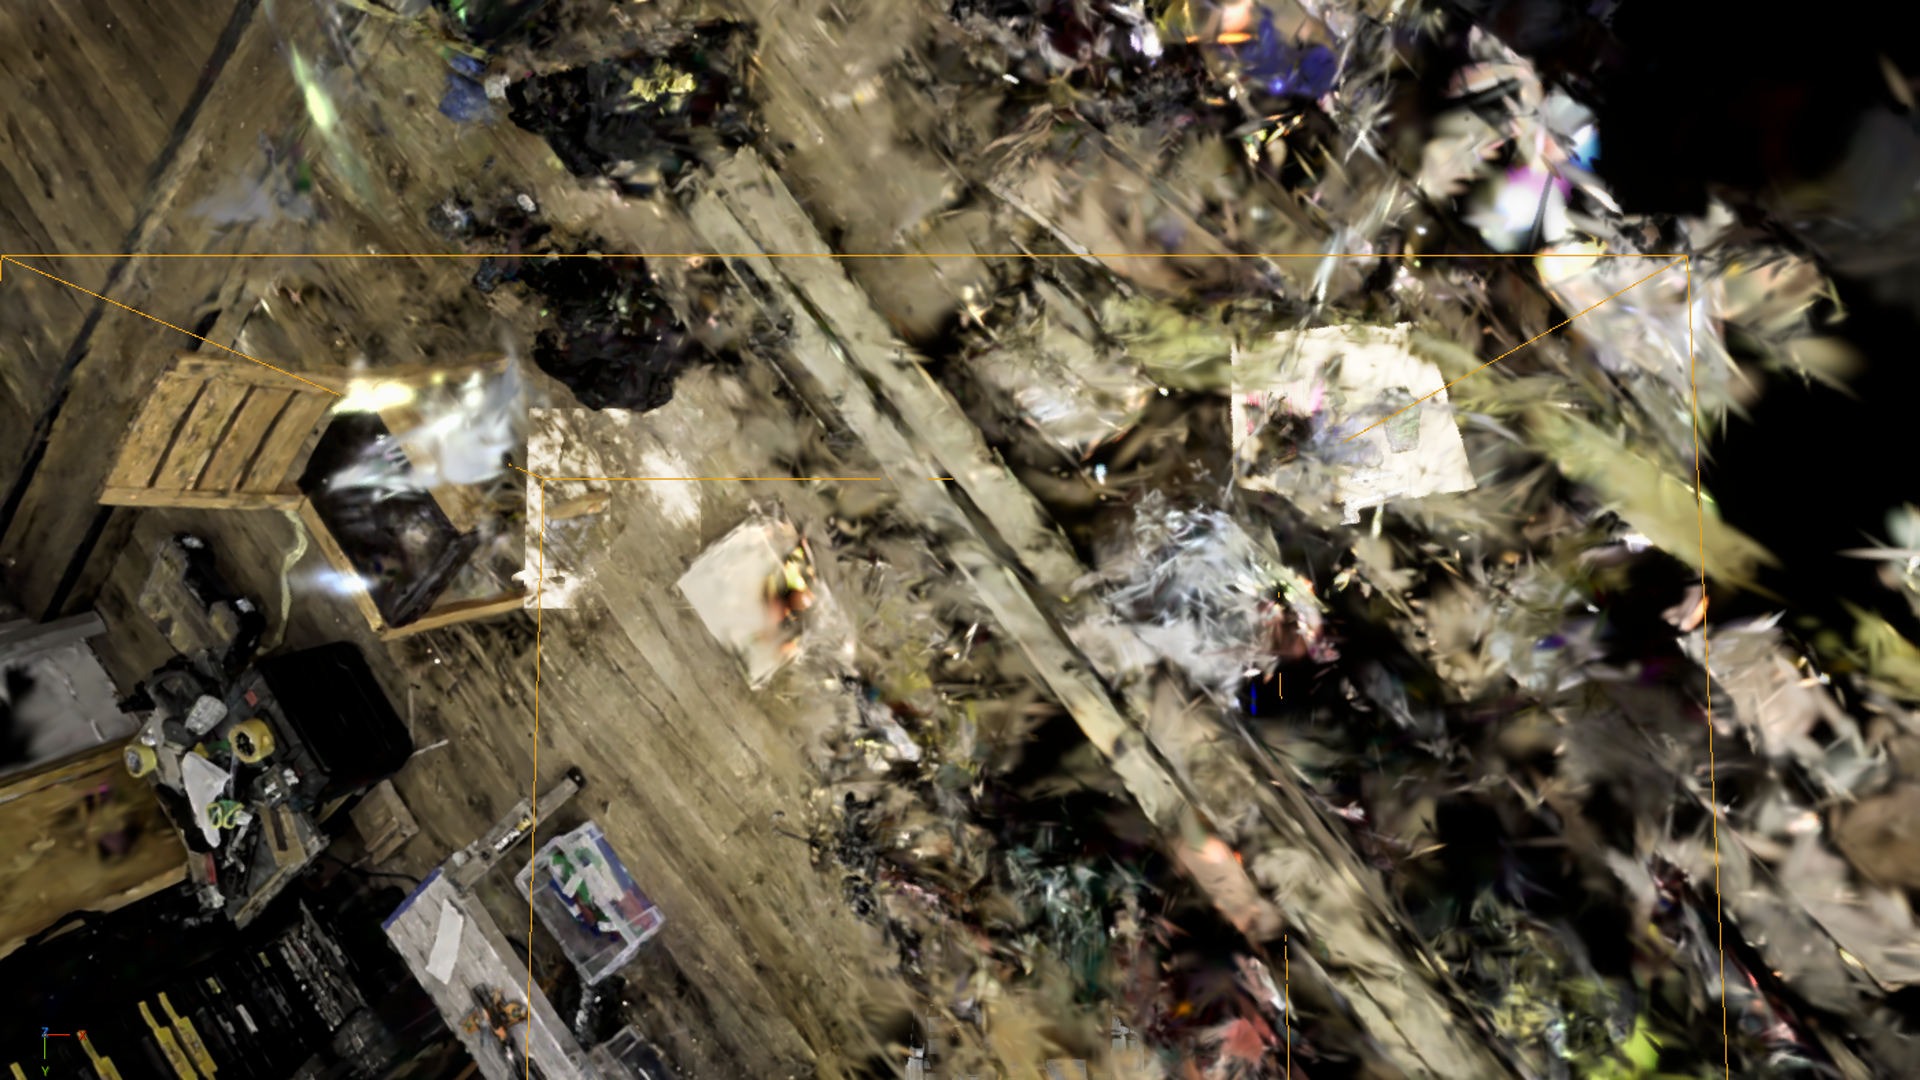
\includegraphics[width=\textwidth]{figures/ue_integrated_dollhouse.png}
  \caption{%
    \textbf{Overhead dollhouse view — integrated UE\,5.8 scene layout.}
    Top-down perspective revealing object placement, room geometry, and
    spatial relationships of the dreamlab scene.
    The dollhouse view is the standard QA checkpoint for scale fidelity
    and object-in-room alignment after \texttt{ue\_place\_prescaled}
    prescaling.
    Resolution: 1920$\times$1080.
  }
  \label{fig:ue_dollhouse}
\end{figure}

% Assumes \graphicspath{{figures/}} is set in the preamble (relative to report/v5/).
%
% Labels (for \ref / \autoref):
%   fig:router           — capture-adaptive router flowchart
%   fig:component_menu   — component-menu status flowchart
%   fig:architecture     — system architecture (container topology)
%   fig:nanogs_room      — NanoGS real-Gaussian splat render (canonical room hero)
%   fig:scene_integrated — fully integrated UE 5.8 scene (room + objects)
%   fig:objects          — TRELLIS.2 object turnaround sheet (chair)
%   fig:ue_come          — CoMe-TSDF mesh game asset in UE (baseline mesh)
%   fig:ue_nanogs        — NanoGS splat render (dreamlab room, 1920x1080)
%   fig:ue_hero          — Hero perspective render (room + placed objects)
%   fig:ue_dollhouse     — Overhead dollhouse view of integrated UE scene

% ──────────────────────────────────────────────────────────────────────────────
% 1. Capture-adaptive router
% ──────────────────────────────────────────────────────────────────────────────
\begin{figure}[htbp]
  \centering
  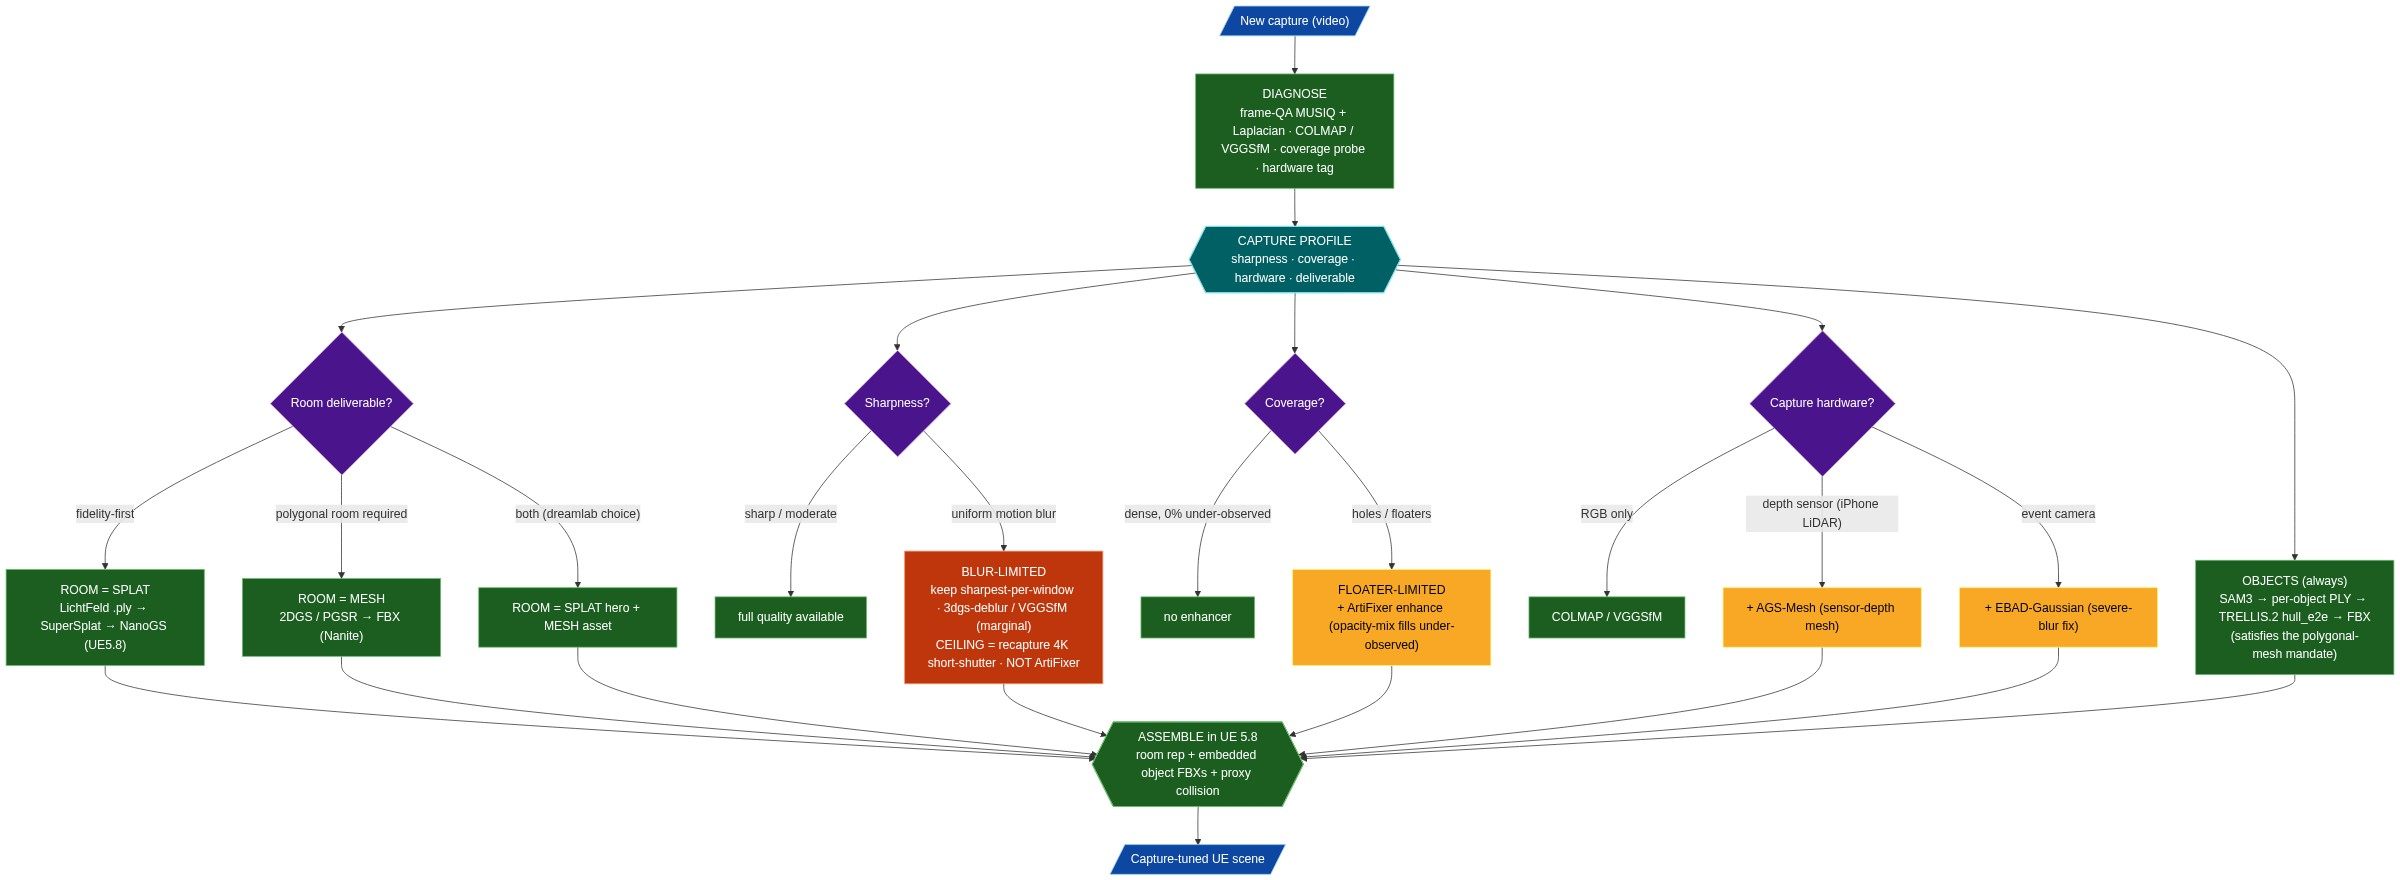
\includegraphics[width=\textwidth]{figures/router.jpg}
  \caption{%
    \textbf{Capture-adaptive router.}
    The pipeline diagnoses each new capture on four axes
    (sharpness via MUSIQ + full-resolution Laplacian, coverage via occupancy probe,
    available hardware, and deliverable type) and selects the configuration that
    fits the bottleneck.
    Green nodes are validated keepers; orange nodes are
    capture-conditional options; red nodes are blur-limited warnings.
    The dreamlab capture routes to Opt\,4 (splat hero + mesh asset + TRELLIS.2 objects)
    with a recapture flag as the quality ceiling.
  }
  \label{fig:router}
\end{figure}

% ──────────────────────────────────────────────────────────────────────────────
% 2. Component-menu flowchart
% ──────────────────────────────────────────────────────────────────────────────
\begin{figure}[htbp]
  \centering
  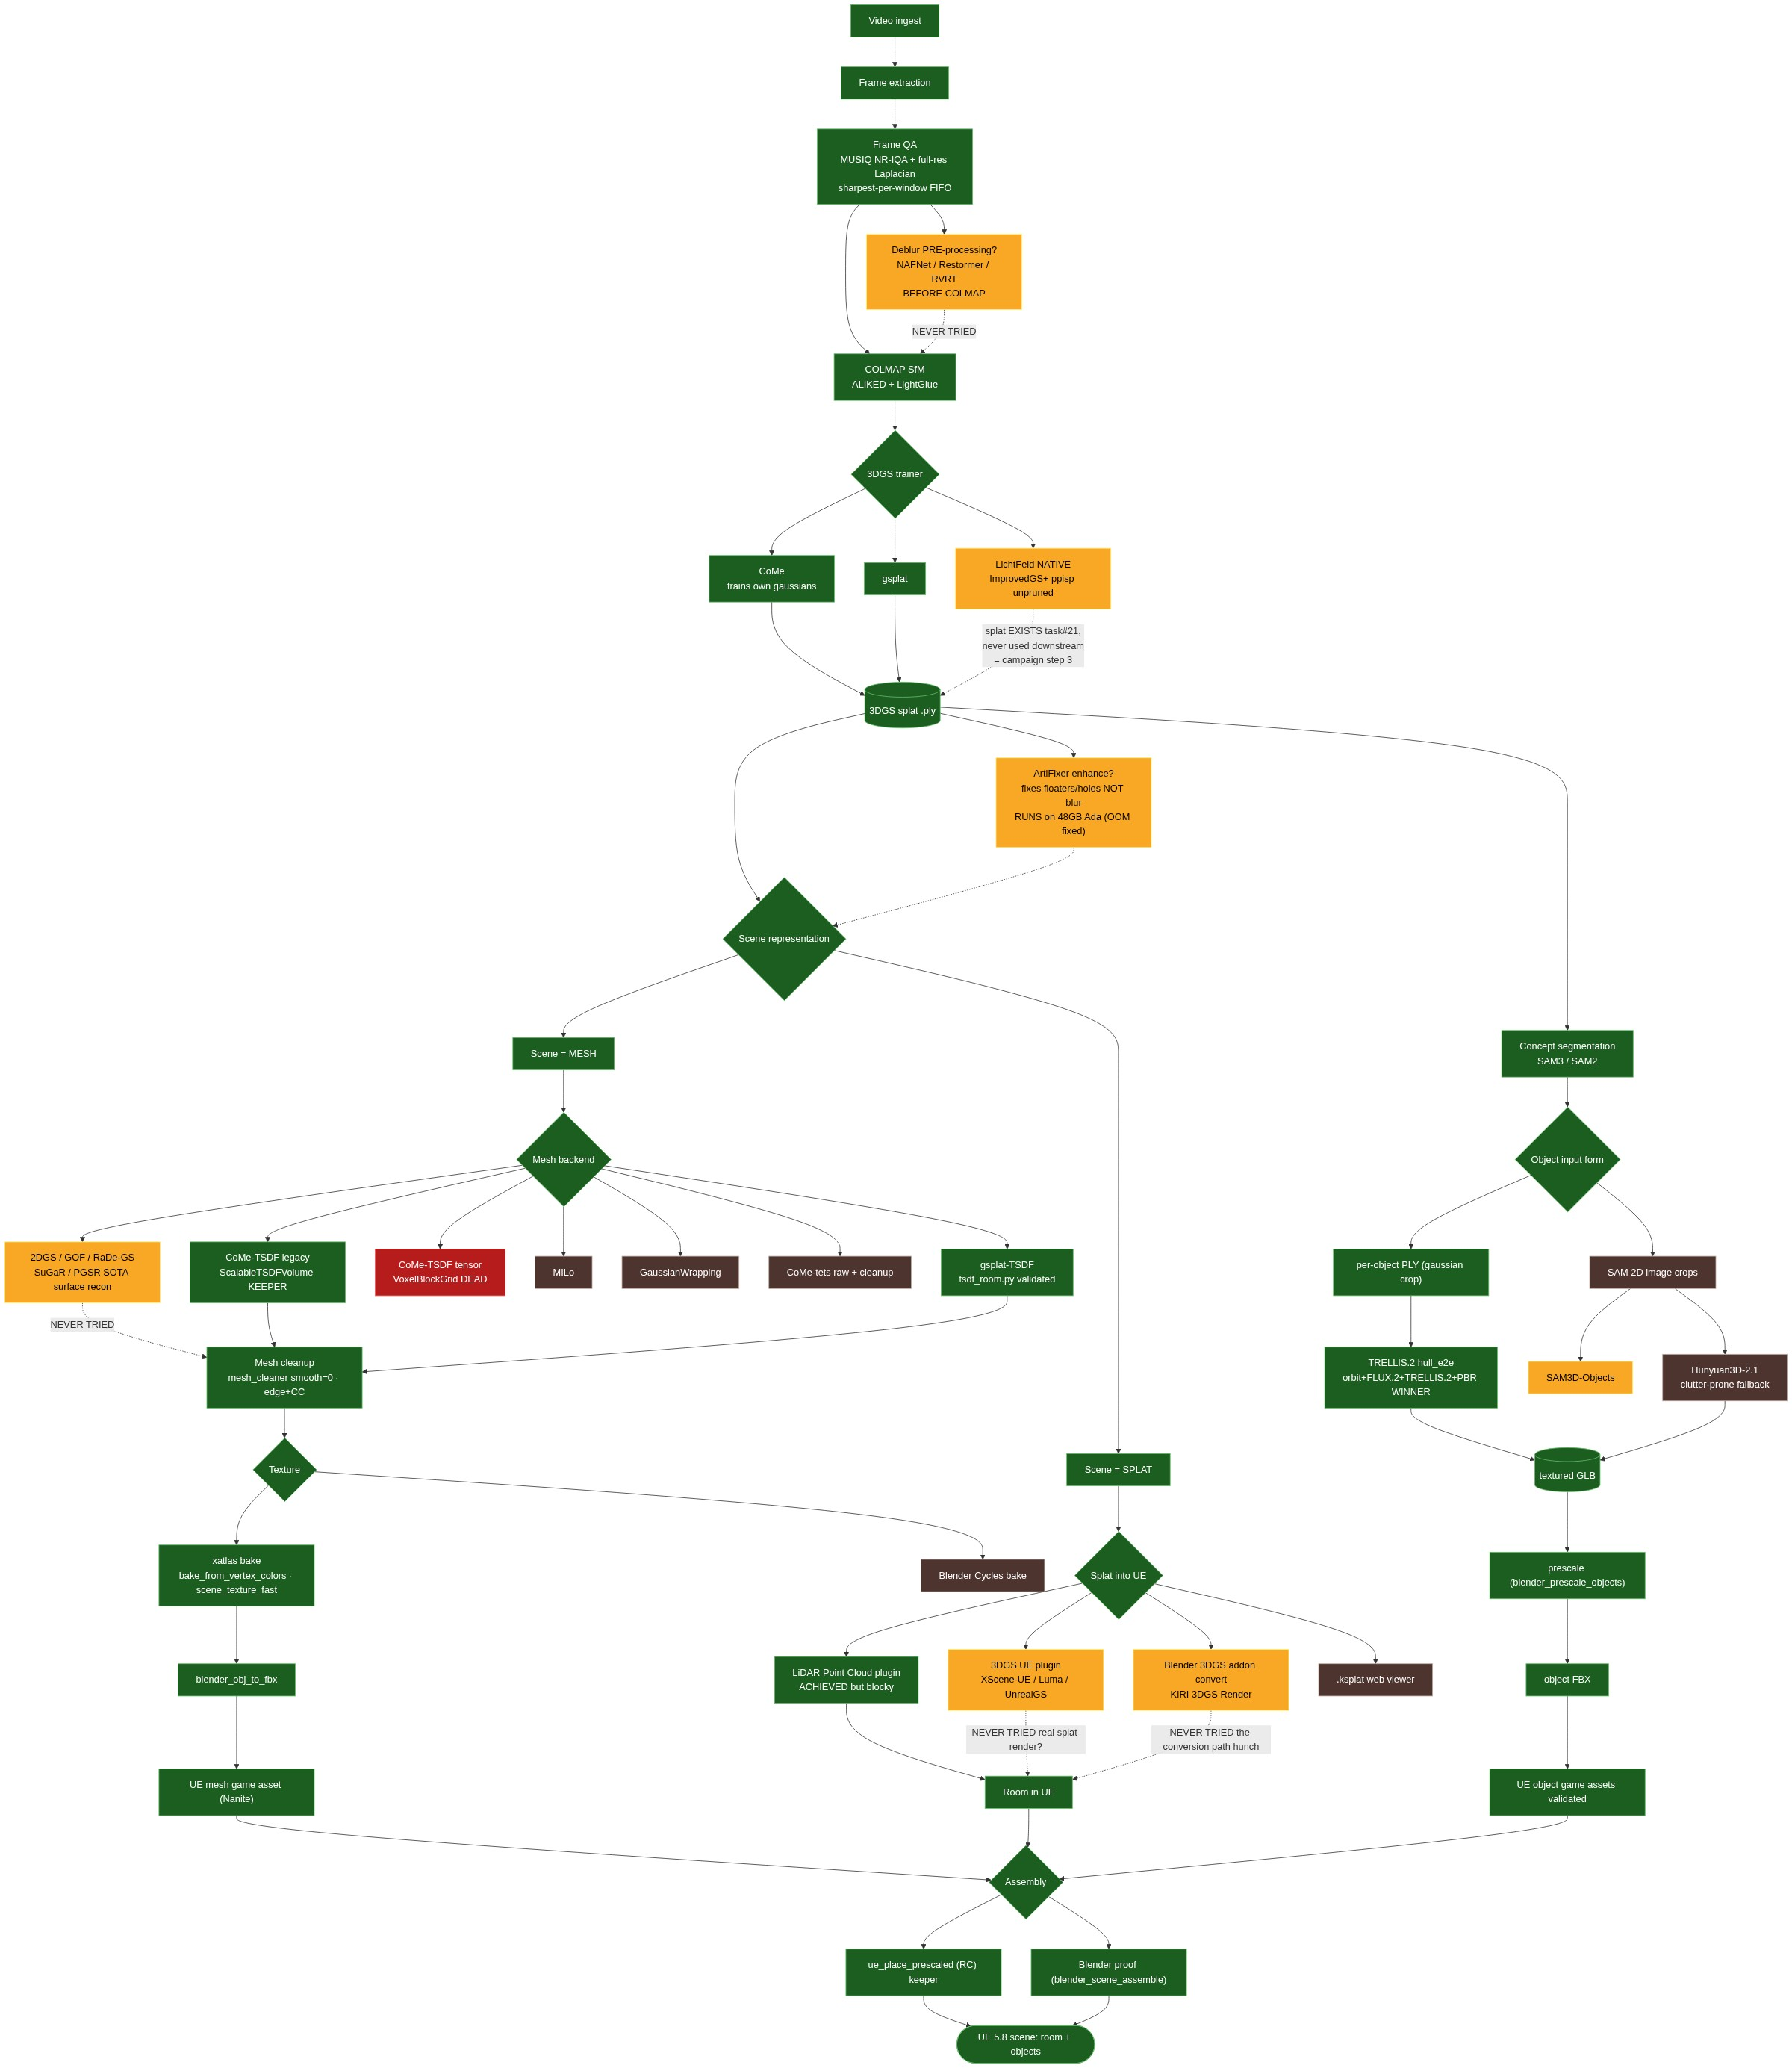
\includegraphics[width=\textwidth]{figures/component_menu.jpg}
  \caption{%
    \textbf{Full component-menu status chart (validated 2026-06-25).}
    Every branch of the Vitrine toolkit from video ingest to UE\,5.8 delivery.
    Colour coding: \emph{green} = validated keeper in active use;
    \emph{brown} = exercised but subordinate / fallback;
    \emph{red} = tried and abandoned;
    \emph{yellow} = plausible, never run.
    The chart is the canonical record of what has and has not been exercised;
    dashed arrows mark paths that remain open research items
    (SAM3D-Objects, BAD-Gaussians deblur, PGSR/2DGS surface reconstruction).
  }
  \label{fig:component_menu}
\end{figure}

% ──────────────────────────────────────────────────────────────────────────────
% 3. System architecture (container topology)
% ──────────────────────────────────────────────────────────────────────────────
\begin{figure}[htbp]
  \centering
  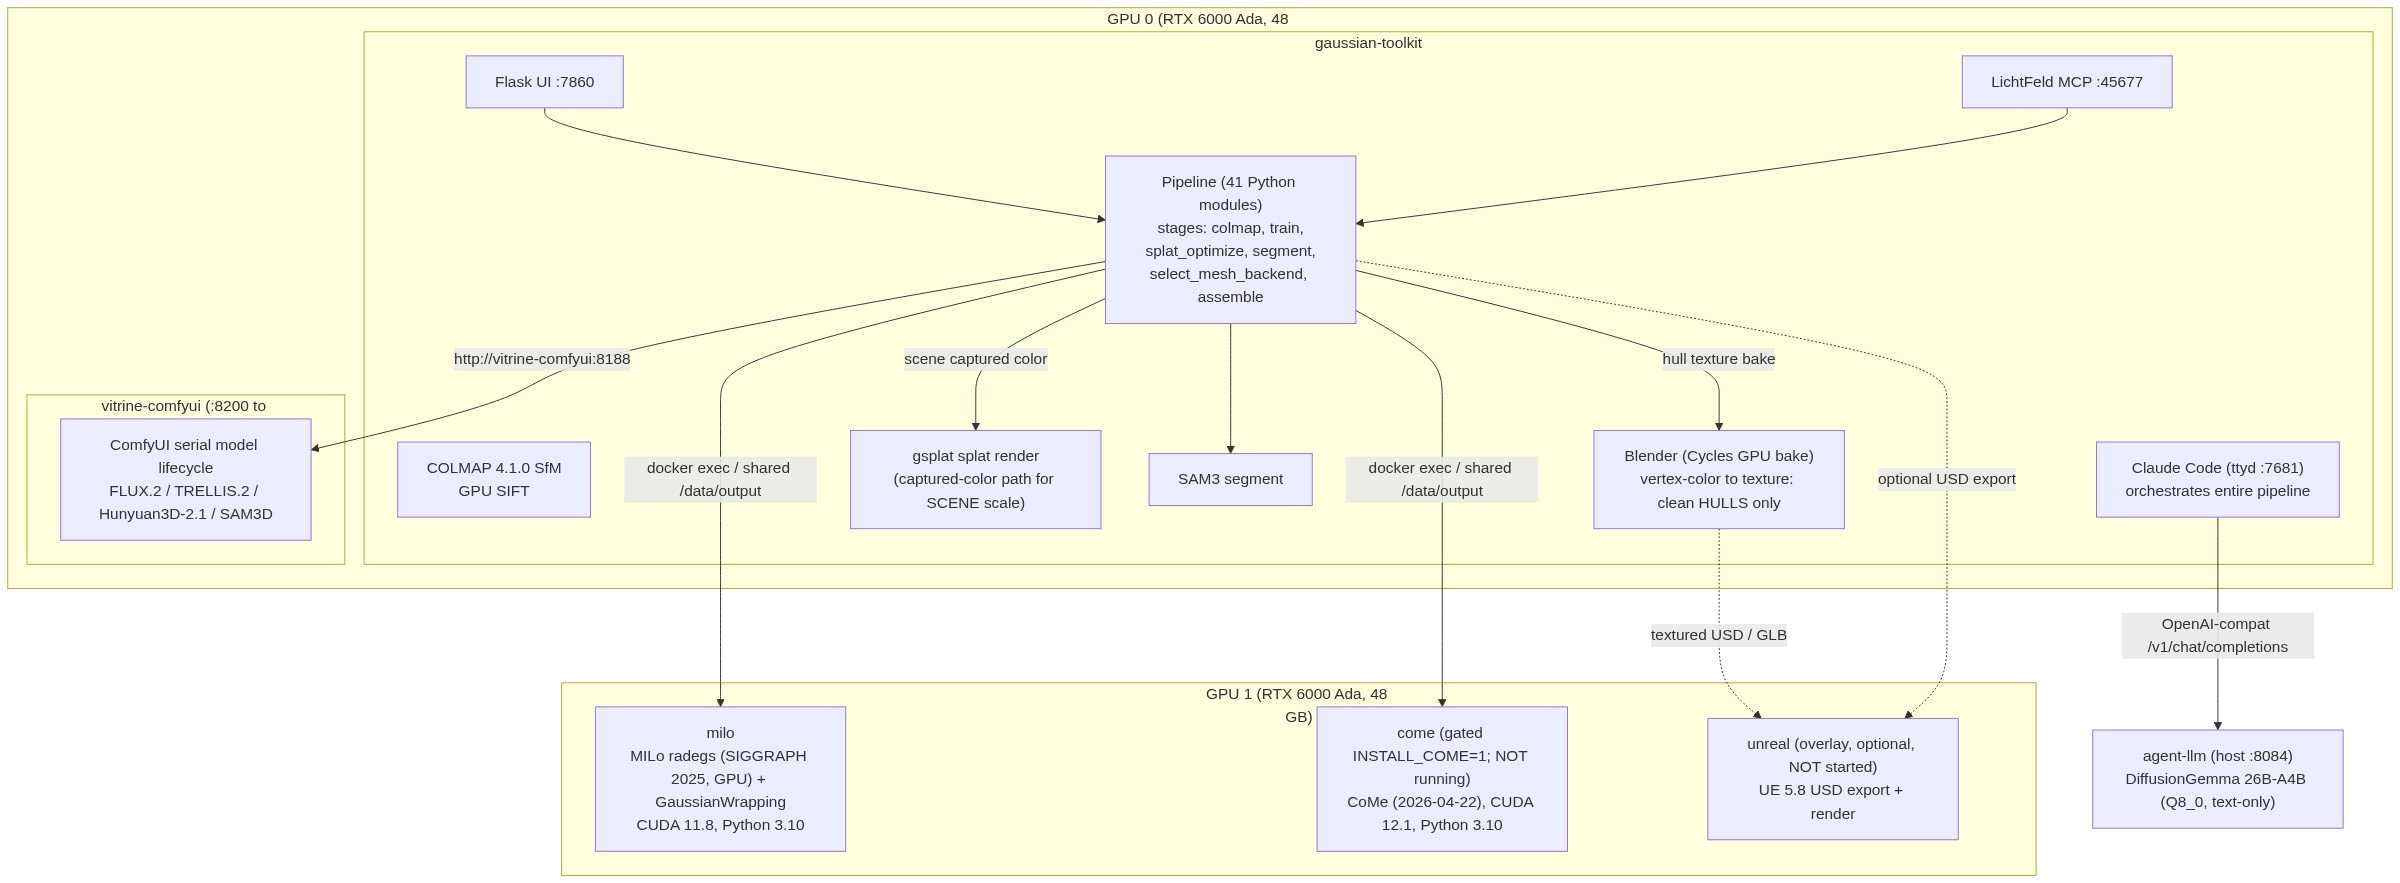
\includegraphics[width=\textwidth]{figures/architecture.jpg}
  \caption{%
    \textbf{Vitrine system architecture — Docker container topology.}
    Two RTX\,6000\,Ada GPUs (48\,GB each) host the six-container stack.
    GPU\,0 runs the \texttt{gaussian-toolkit} orchestrator (COLMAP, LichtFeld
    3DGS, SAM3, Flask\,UI, LichtFeld\,MCP on port\,45677) and
    \texttt{vitrine-comfyui} (FLUX.2\,/\,TRELLIS.2\,/\,Hunyuan3D-2.1, serial
    model lifecycle).
    GPU\,1 hosts the \texttt{milo} sidecar (MILo radegs, CUDA\,11.8) and the
    optional \texttt{come} (CoMe, CUDA\,12.1) and \texttt{unreal} (UE\,5.8)
    overlay containers.
    DiffusionGemma\,26B-A4B runs on the host at port\,8084 as the local text
    reasoner.
    All pipeline containers share \texttt{v2g-net}; the agentbox (Claude Code)
    reaches them via the shared \texttt{visionclaw\_network}.
  }
  \label{fig:architecture}
\end{figure}

% ──────────────────────────────────────────────────────────────────────────────
% 4. NanoGS room splat (docs canonical hero)
% ──────────────────────────────────────────────────────────────────────────────
\begin{figure}[htbp]
  \centering
  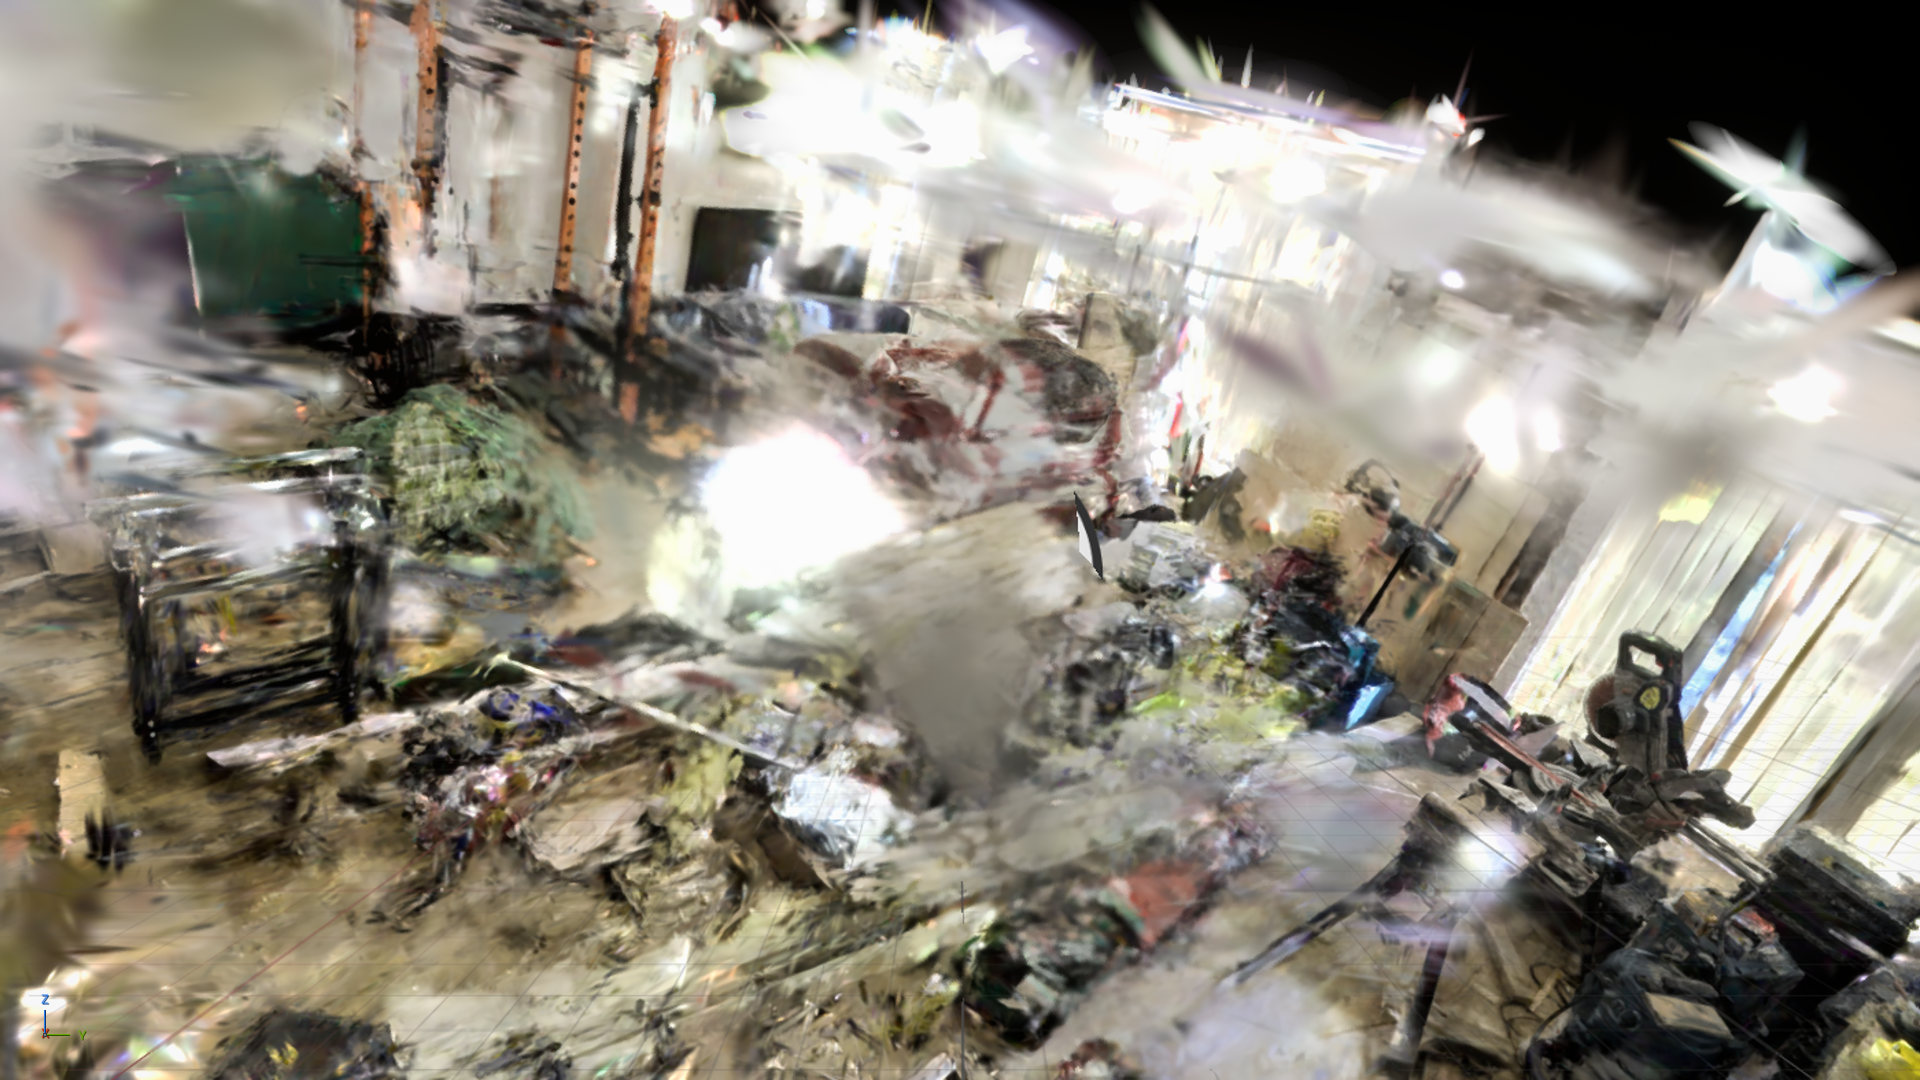
\includegraphics[width=\textwidth]{figures/nanogs_room_splat.png}
  \caption{%
    \textbf{Dreamlab room — NanoGS real-Gaussian splat render (canonical hero).}
    The LichtFeld-native \texttt{splat\_30000.ply}, cleaned via SuperSplat and
    loaded into the NanoGS\,(MIT) UE\,5.8 plugin, rendered at 1920$\times$1080.
    This replaces the earlier LiDAR point-cloud workaround and constitutes
    campaign step\,3: lean-on-LichtFeld native output for the room representation.
    Motion-blur softness in the source splat reflects the dreamlab capture
    constraint (MUSIQ $\approx$ 31); recapture at 4\,K\,/\,short shutter is the
    ceiling lever, not a pipeline limitation.
  }
  \label{fig:nanogs_room}
\end{figure}

% ──────────────────────────────────────────────────────────────────────────────
% 5. Fully integrated UE 5.8 scene
% ──────────────────────────────────────────────────────────────────────────────
\begin{figure}[htbp]
  \centering
  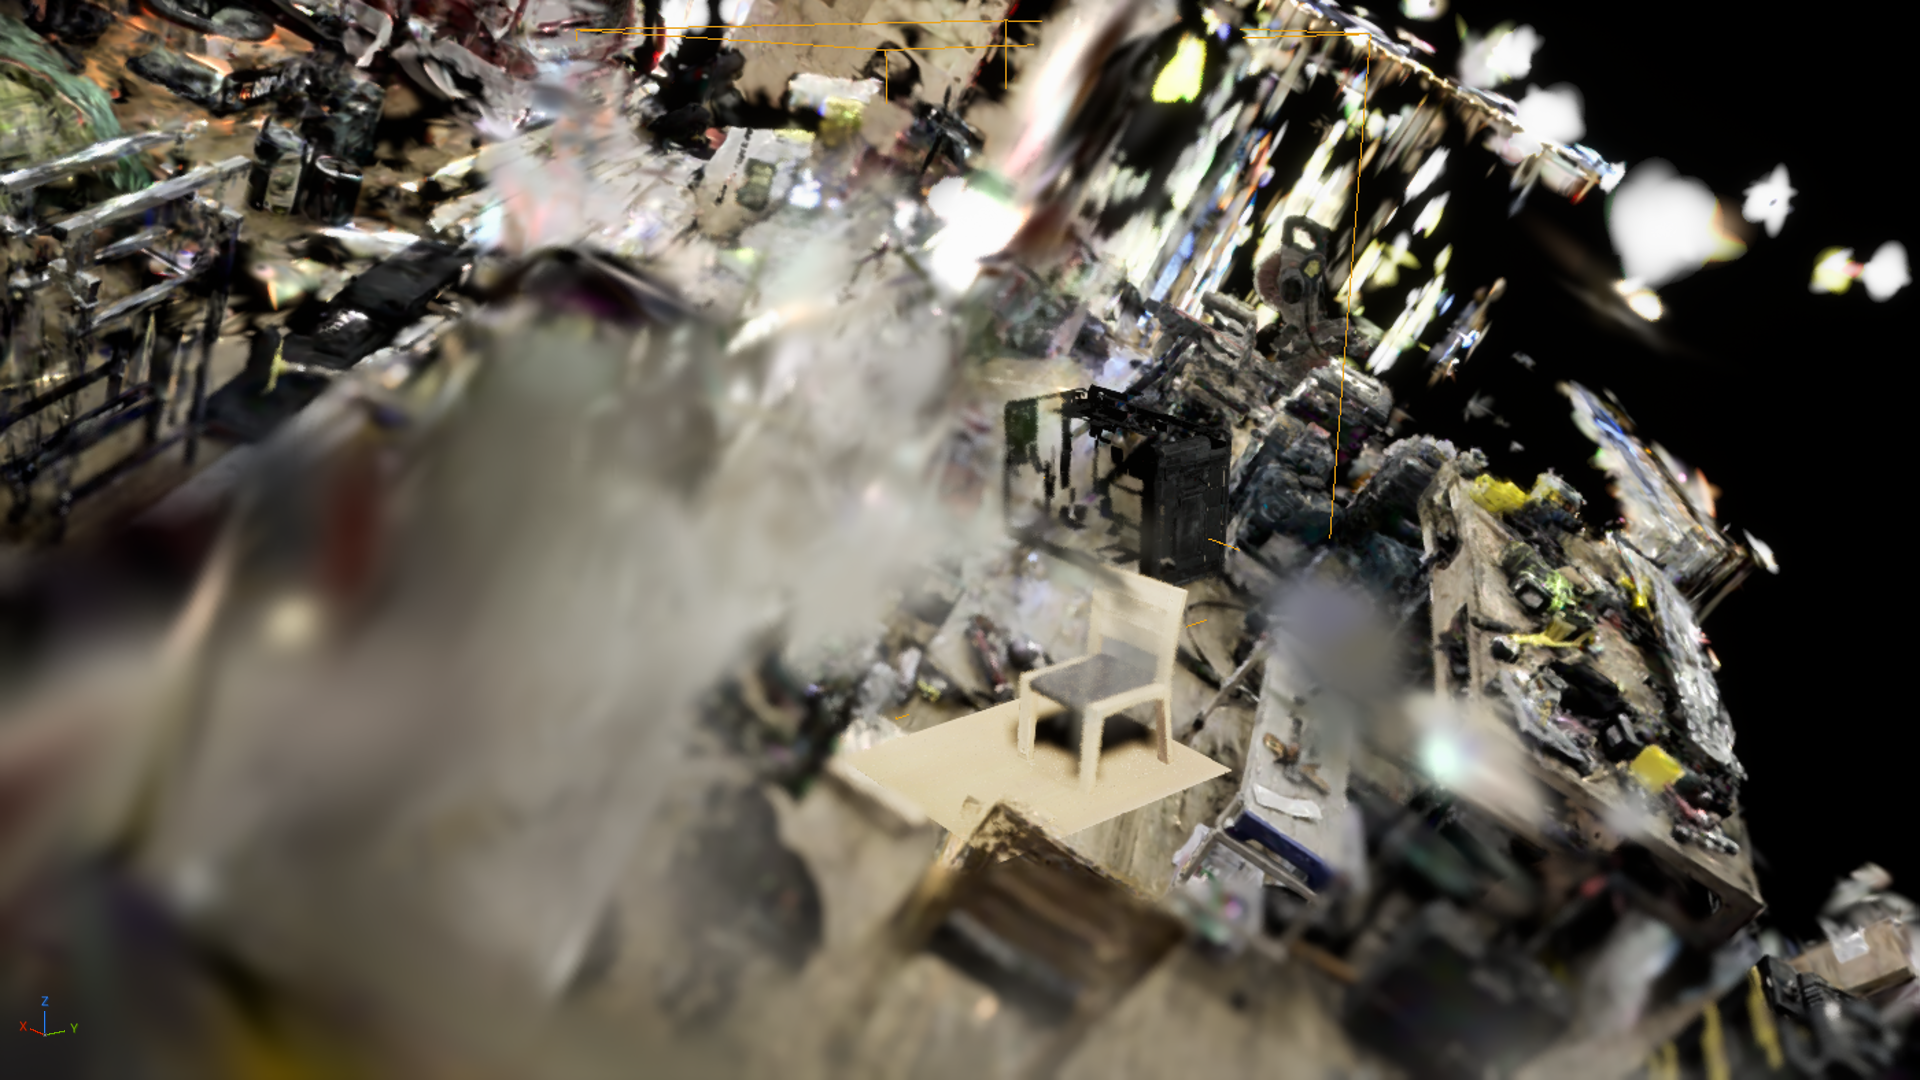
\includegraphics[width=\textwidth]{figures/scene_integrated.png}
  \caption{%
    \textbf{Integrated UE\,5.8 scene — room splat with placed TRELLIS.2 object FBXs.}
    The assembled deliverable: NanoGS splat room (hero representation) with
    chair, vacuum, and toolbox FBXs (TRELLIS.2 \texttt{hull\_e2e},
    prescaled via \texttt{blender\_prescale\_objects}) placed by
    \texttt{ue\_place\_prescaled}.
    Objects are Nanite game assets with baked PBR textures; the room splat
    renders real Gaussians.
    This image is the \emph{docs} canonical integrated-scene reference.
  }
  \label{fig:scene_integrated}
\end{figure}

% ──────────────────────────────────────────────────────────────────────────────
% 6. TRELLIS.2 object turnaround sheet (chair)
% ──────────────────────────────────────────────────────────────────────────────
\begin{figure}[htbp]
  \centering
  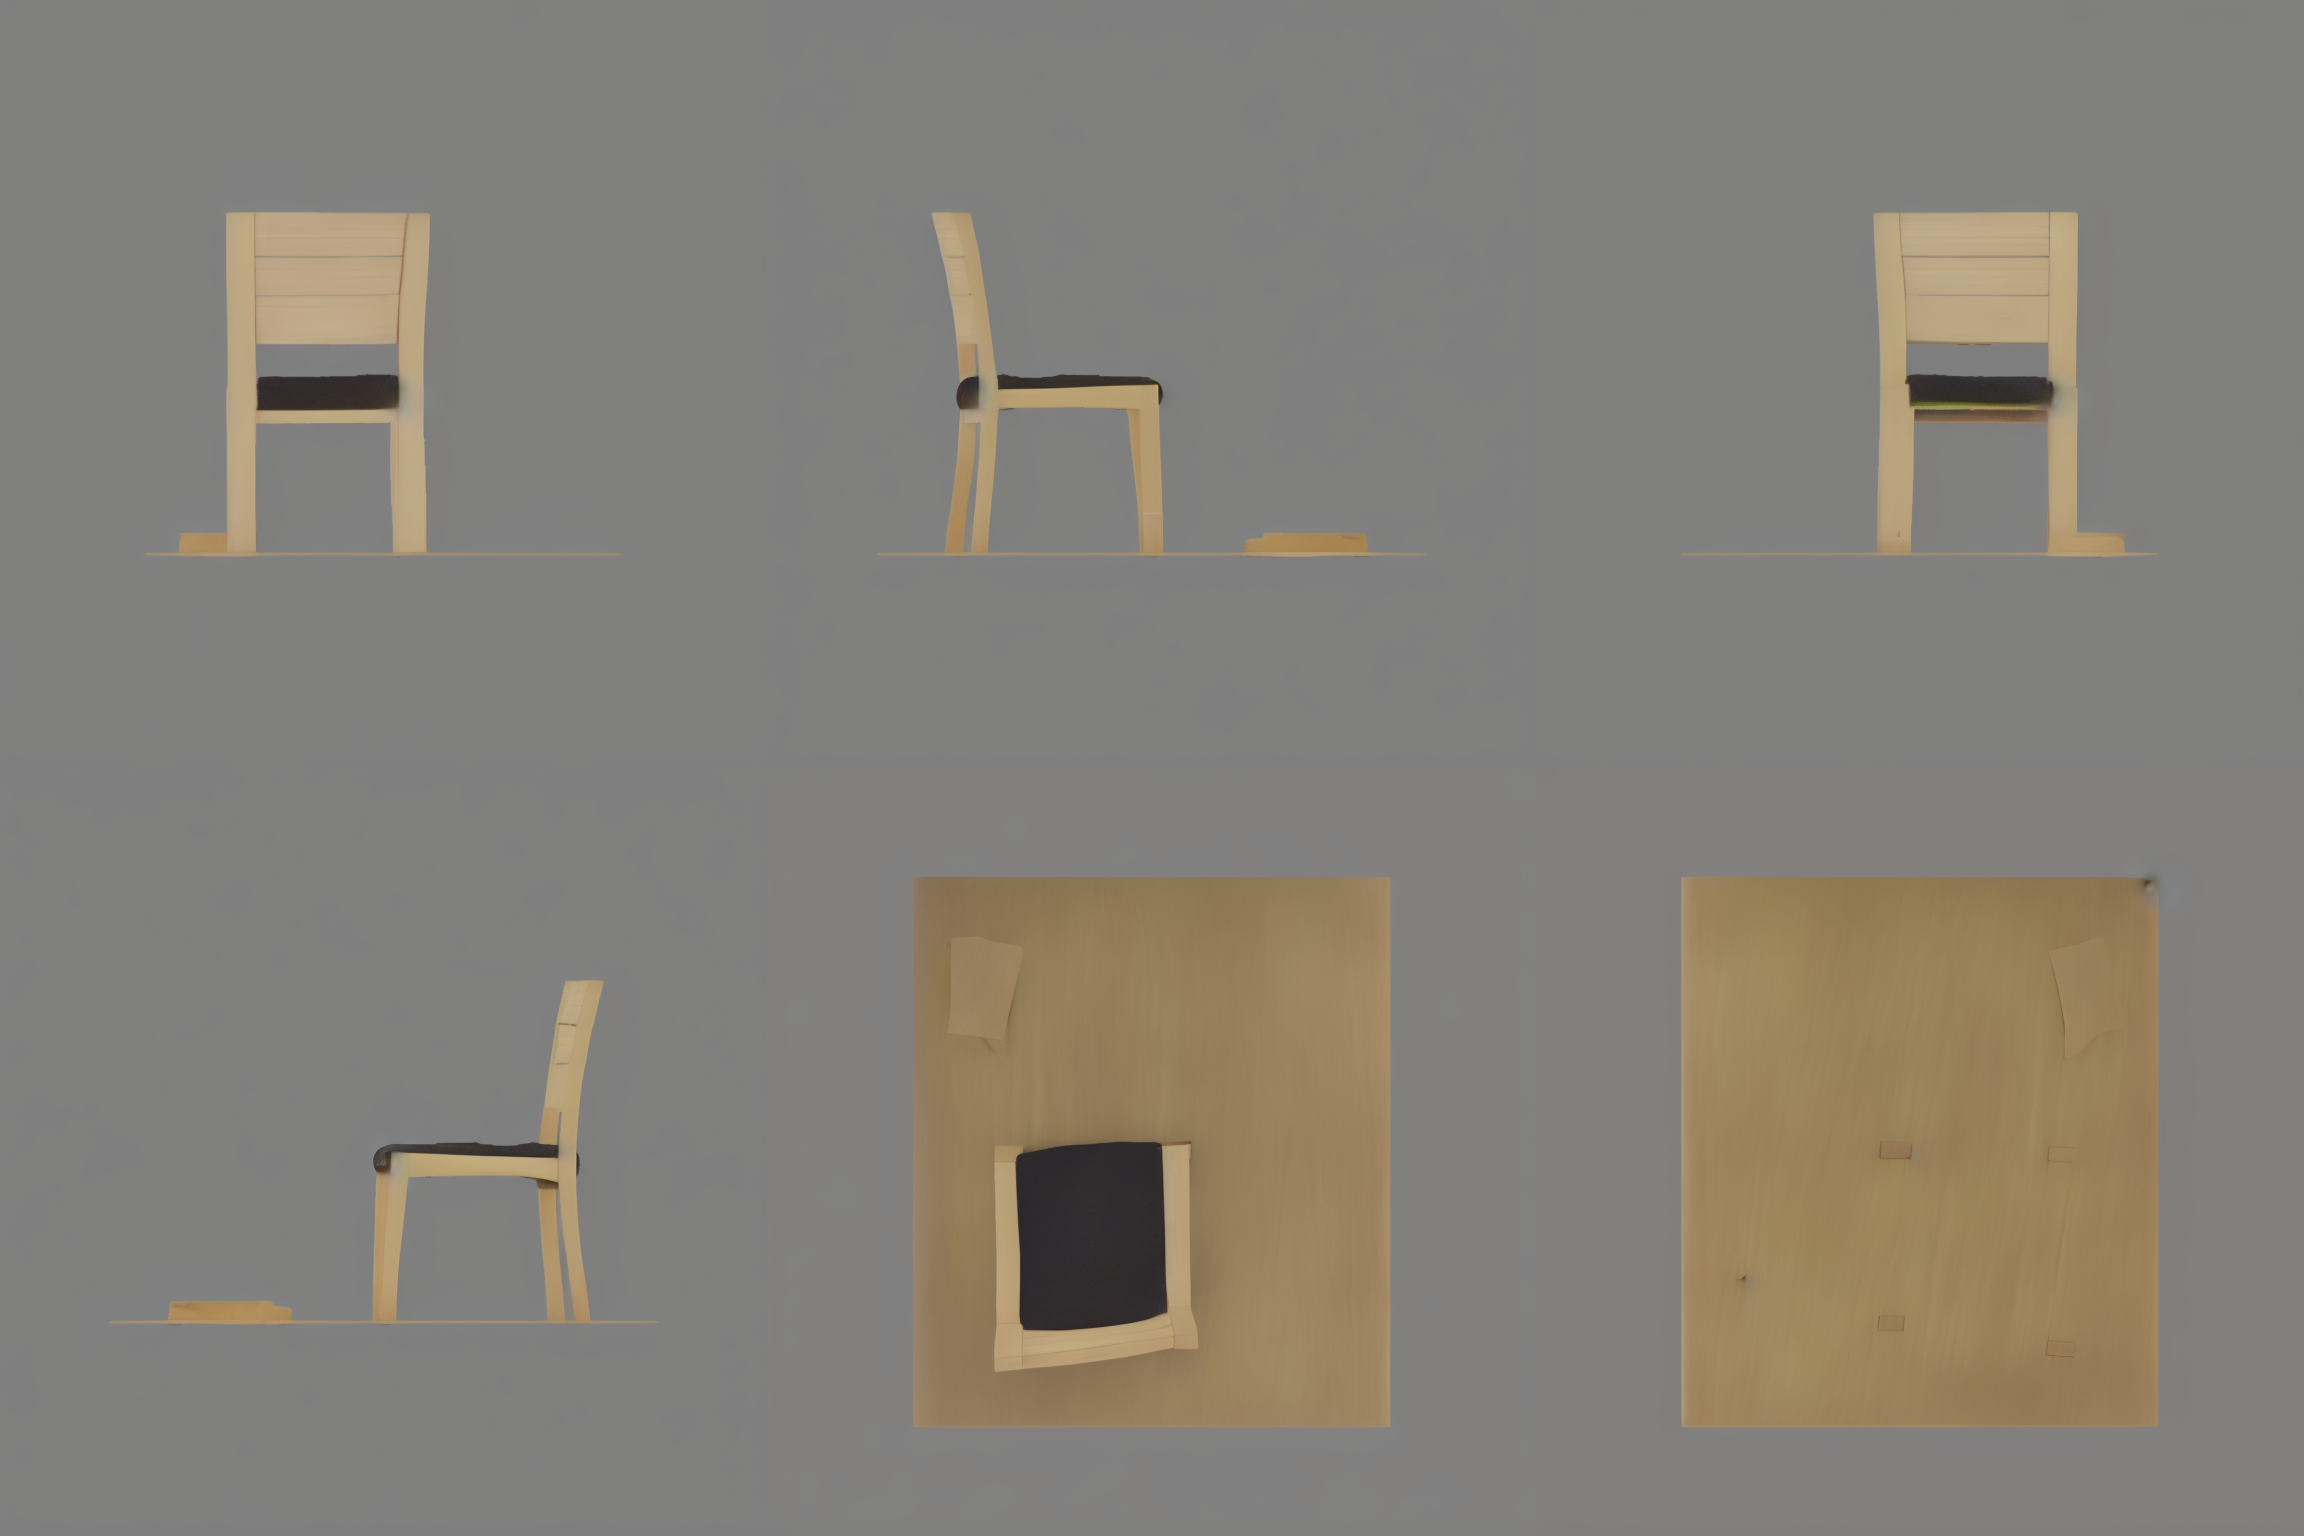
\includegraphics[width=\textwidth]{figures/chair_turnaround_sheet.png}
  \caption{%
    \textbf{TRELLIS.2 object reconstruction — chair turnaround sheet.}
    Multi-view orbit render of the textured GLB mesh produced by the
    \texttt{hull\_e2e} workflow: per-object SAM3 PLY crop $\to$ FLUX.2-dev
    view-inpainting $\to$ TRELLIS.2-4B mesh $\to$ PBR-baked GLB $\to$ FBX
    (Nanite game asset).
    The chair is rated \emph{good}; vacuum and toolbox likewise passed
    the object reconstruction gate (4/8 objects in this batch).
    Resolution: 2304$\times$1536.
  }
  \label{fig:objects}
\end{figure}

% ──────────────────────────────────────────────────────────────────────────────
% 7. CoMe-TSDF mesh in UE (baseline mesh deliverable)
% ──────────────────────────────────────────────────────────────────────────────
\begin{figure}[htbp]
  \centering
  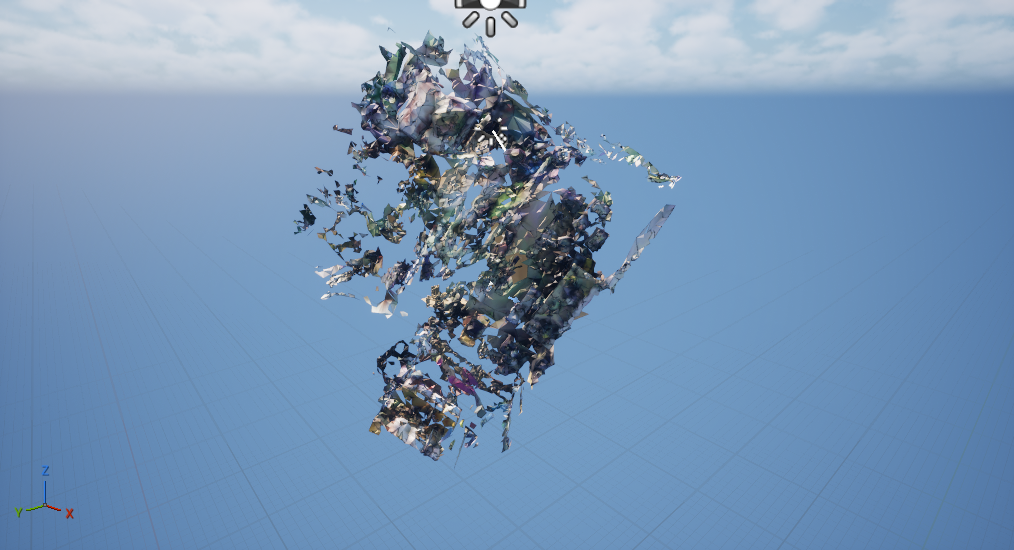
\includegraphics[width=\textwidth]{figures/ue_come_final.png}
  \caption{%
    \textbf{CoMe-TSDF room mesh game asset in UE\,5.8 (baseline mesh deliverable).}
    The scene-mesh branch: CoMe legacy \texttt{ScalableTSDFVolume} extraction,
    \texttt{mesh\_cleaner} (smooth=0, edge-length + connected-component cleanup),
    xatlas bake (\texttt{bake\_from\_vertex\_colors}), \texttt{blender\_obj\_to\_fbx},
    imported as a Nanite mesh.
    Characteristic TSDF blockiness on flat walls is visible; this image
    motivates the re-spine to NanoGS as the default room representation for
    blur-limited captures.
    Resolution: 1014$\times$550.
  }
  \label{fig:ue_come}
\end{figure}

% ──────────────────────────────────────────────────────────────────────────────
% 8. NanoGS splat render (1920×1080 B-view)
% ──────────────────────────────────────────────────────────────────────────────
\begin{figure}[htbp]
  \centering
  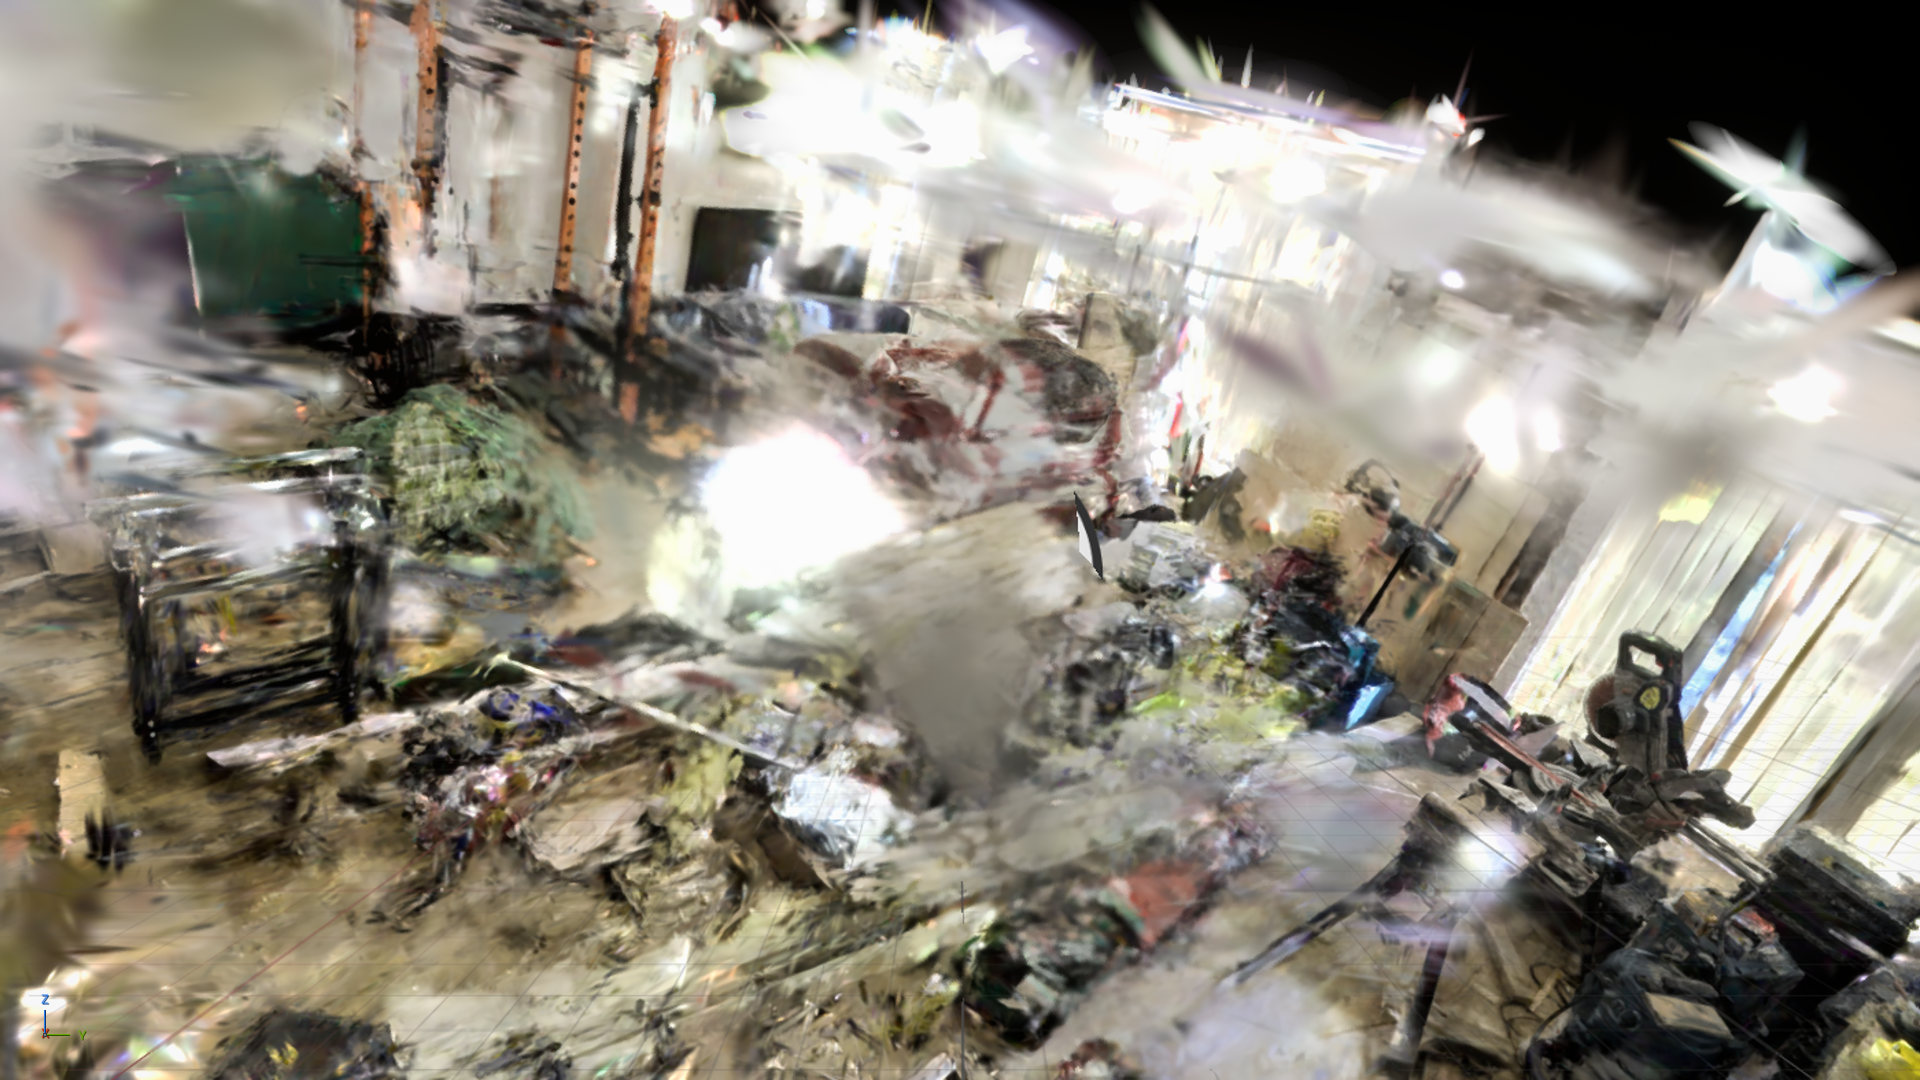
\includegraphics[width=\textwidth]{figures/ue_nanogs_room_B.png}
  \caption{%
    \textbf{NanoGS real-Gaussian splat in UE\,5.8 — interior view (B).}
    Second viewpoint of the NanoGS splat room, demonstrating depth and
    parallax of real Gaussian rendering at 1920$\times$1080.
    Comparison with Figure~\ref{fig:ue_come} illustrates the quality
    improvement of splat-hero over TSDF mesh for a motion-blur-limited
    capture: the splat faithfully preserves captured radiance;
    the mesh introduces geometric artefacts irrelevant to the capture.
  }
  \label{fig:ue_nanogs}
\end{figure}

% ──────────────────────────────────────────────────────────────────────────────
% 9. Hero perspective render (room + placed objects)
% ──────────────────────────────────────────────────────────────────────────────
\begin{figure}[htbp]
  \centering
  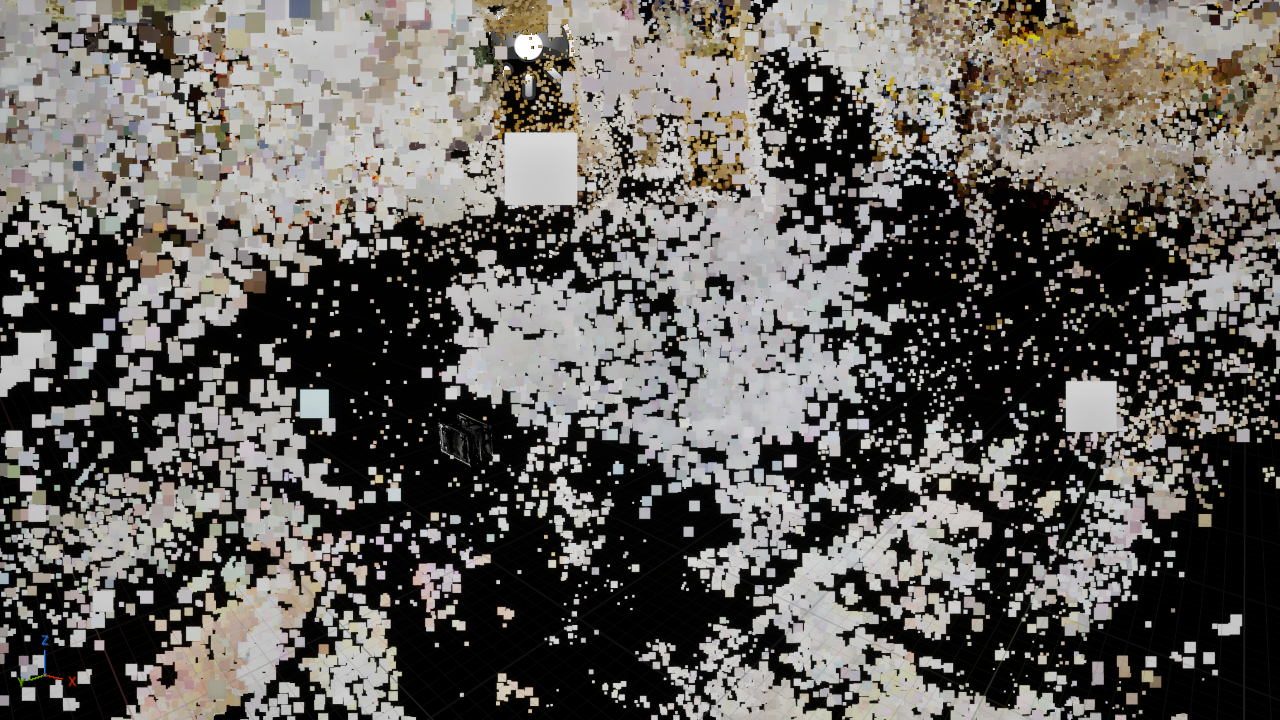
\includegraphics[width=\textwidth]{figures/ue_final_hero.png}
  \caption{%
    \textbf{Hero perspective render — dreamlab room with placed object FBXs.}
    A cinematic view of the assembled UE\,5.8 scene from the validated
    end-to-end run (2026-06-22): TSDF-mesh room (CoMe, pre-NanoGS re-spine)
    with TRELLIS.2 object FBXs placed by \texttt{ue\_place\_prescaled}.
    Resolution: 1280$\times$720.
    Serves as the primary before/after reference for evaluating the
    NanoGS re-spine (Figure~\ref{fig:nanogs_room}).
  }
  \label{fig:ue_hero}
\end{figure}

% ──────────────────────────────────────────────────────────────────────────────
% 10. Overhead dollhouse view
% ──────────────────────────────────────────────────────────────────────────────
\begin{figure}[htbp]
  \centering
  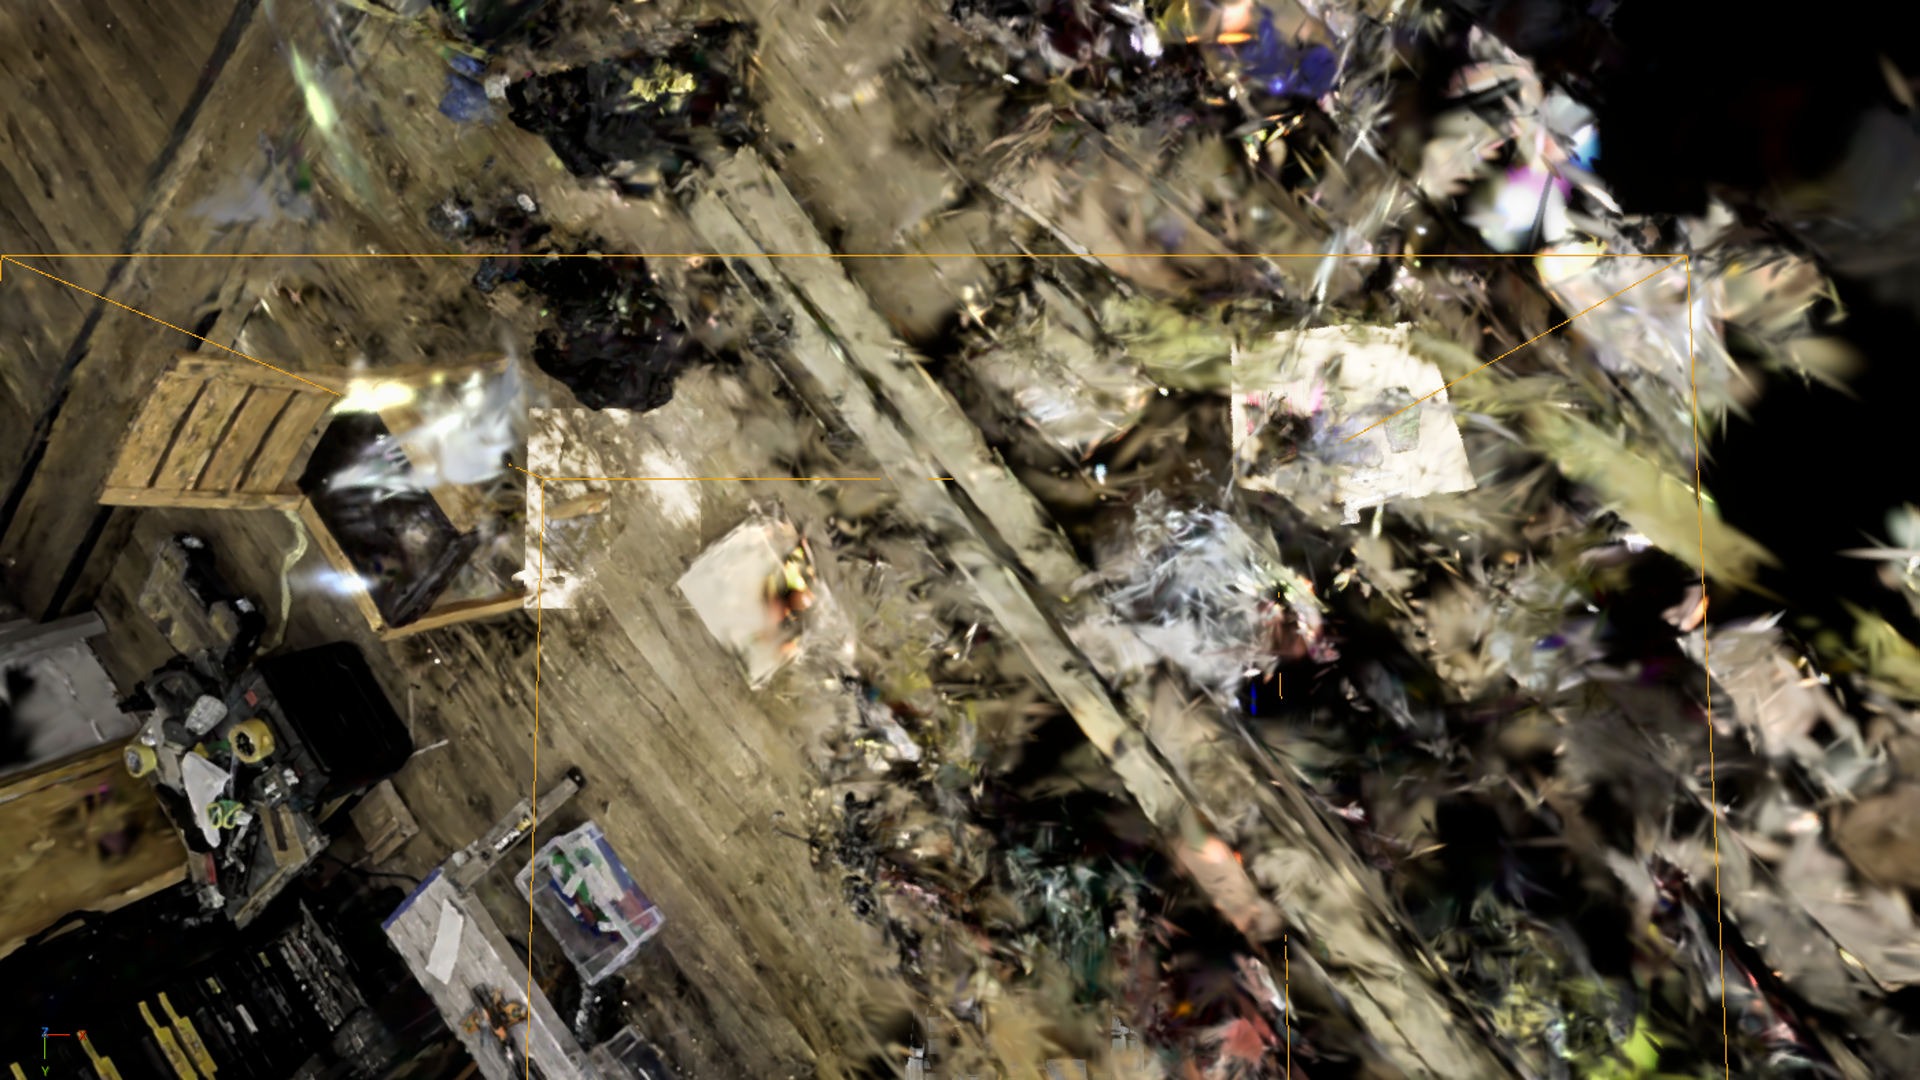
\includegraphics[width=\textwidth]{figures/ue_integrated_dollhouse.png}
  \caption{%
    \textbf{Overhead dollhouse view — integrated UE\,5.8 scene layout.}
    Top-down perspective revealing object placement, room geometry, and
    spatial relationships of the dreamlab scene.
    The dollhouse view is the standard QA checkpoint for scale fidelity
    and object-in-room alignment after \texttt{ue\_place\_prescaled}
    prescaling.
    Resolution: 1920$\times$1080.
  }
  \label{fig:ue_dollhouse}
\end{figure}
